\documentclass[anon,12pt]{colt2026} % Anonymized submission
%\documentclass[final,12pt]{colt2026} % Include author names

% The following packages will be automatically loaded:
% amsmath, amssymb, natbib, graphicx, url, algorithm2e

\title[Transformer Hessians]{Closing the Curvature Gap: Full Transformer Hessians}
\usepackage{times}
% Use \Name{Author Name} to specify the name.
% If the surname contains spaces, enclose the surname
% in braces, e.g. \Name{John {Smith Jones}} similarly
% if the name has a "von" part, e.g \Name{Jane {de Winter}}.
% If the first letter in the forenames is a diacritic
% enclose the diacritic in braces, e.g. \Name{{\'E}louise Smith}
\usepackage[utf8]{inputenc} % allow utf-8 input
\usepackage[T1]{fontenc}    % use 8-bit T1 fonts
\usepackage{hyperref}       % hyperlinks
\usepackage{url}            % simple URL typesetting
\usepackage{booktabs}       % professional-quality tables
\usepackage{amsfonts}       % blackboard math symbols
\usepackage{nicefrac}       % compact symbols for 1/2, etc.
\usepackage{microtype}      % microtypography
\usepackage{xcolor}         % colors

%%%

\usepackage{subcaption}
\usepackage{graphicx}
\usepackage{multirow}
\usepackage{amsmath,amssymb,amsfonts}
% \usepackage{amsthm}
\usepackage{mathrsfs}
% \usepackage{xcolor}
\usepackage[dvipsnames]{xcolor}
\usepackage{textcomp}
\usepackage{manyfoot}
\usepackage{booktabs}
\usepackage{algorithm}
\usepackage{algorithmicx}
\usepackage{algpseudocode}
\usepackage{listings}
\usepackage{diagbox}
\usepackage{wrapfig}

\graphicspath{{figs}}

%%% TIKZ %%%

\usepackage{tikz}
\usetikzlibrary{arrows.meta,calc,fit,positioning,backgrounds}

\usetikzlibrary{matrix}                  % For "matrix of math nodes"
\usetikzlibrary{positioning}             % For "right=3cm of W"
\usetikzlibrary{arrows.meta}             % For arrow styles
\usetikzlibrary{decorations.pathreplacing} % For the curly braces
\usetikzlibrary{positioning, decorations.pathreplacing}

\definecolor{ff}{RGB}{193,231,247}   % FeedForward
\definecolor{sa}{RGB}{255,225,188}  % Self-Attention
\definecolor{ln}{RGB}{242,244,192}   % LayerNorm

\definecolor{plotBlue}{RGB}{31,119,180}  % as in matplotlib
\definecolor{plotOrange}{RGB}{255,127,14}  % as in matplotlib

%%%%%%%%%%%%

% \newtheorem{theorem}{Theorem} % continuous numbers
%%\newtheorem{theorem}{Theorem}[section] % sectionwise numbers
%% optional argument [theorem] produces theorem numbering sequence instead of independent numbers for Proposition
% \newtheorem{proposition}[theorem]{Proposition}% 
%%\newtheorem{proposition}{Proposition} % to get separate numbers for theorem and proposition etc.

% \newtheorem{example}{Example}
% \newtheorem{remark}{Remark}

% \newtheorem{definition}{Definition}
\newtheorem{assumption}{Assumption}

% \newtheorem{lemma}{Lemma}
% \newtheorem{proposition}{Proposition}

\newtheorem{property}{Property}
% Two authors with the same address
% \coltauthor{\Name{Author Name1} \Email{abc@sample.com}\and
%  \Name{Author Name2} \Email{xyz@sample.com}\\
%  \addr Address}

% Three or more authors with the same address:
% \coltauthor{\Name{Author Name1} \Email{an1@sample.com}\\
%  \Name{Author Name2} \Email{an2@sample.com}\\
%  \Name{Author Name3} \Email{an3@sample.com}\\
%  \addr Address}

% Authors with different addresses:
\coltauthor{%
 \Name{Author Name1} \Email{abc@sample.com}\\
 \addr Address 1
 \AND
 \Name{Author Name2} \Email{xyz@sample.com}\\
 \addr Address 2%
}

\begin{document}


\maketitle

\begin{abstract}
The optimization landscape of Transformer models remains poorly understood despite their widespread adoption. While recent studies have derived curvature properties for isolated self-attention mechanisms, a comprehensive theoretical characterization of the full Transformer block, accounting for the interactions between Layer Normalization, Feed-Forward Networks (FFNs), and residual connections, is missing. In this work, we close this gap by deriving the exact, closed-form Hessian for the complete Transformer architecture under arbitrary twice-differentiable loss functions. We utilize rigorous matrix calculus to handle the non-linearities of LayerNorm and row-wise activations, establishing explicit spectral norm bounds for the resulting Hessian blocks. Our results characterize the extreme heterogeneity of the optimization landscape, identifying the distinct curvature contributions of specific sub-layers. Furthermore, we establish a theoretical link between signal magnitude and landscape sharpness, providing a rigorous foundation for understanding architectural stability, convergence dynamics, and the necessity of adaptive optimization methods in large-scale deep learning.
\end{abstract}

\begin{keywords}%
  Transformer Hessians, Layer Normalization, Matrix Calculus, Loss landscape, Optimization geometry.
\end{keywords}

% \textbf{Keywords:} Transformer Hessians, Layer Normalization, Scaling laws, Convergence dynamics, Loss landscape, Optimization geometry.

% \section{Introduction}\label{sec:intro}

% \begin{figure}[h]
%     \centering
%     \begin{tikzpicture}[
%       >=Latex,
%       lossA/.style={ultra thick, plotBlue},
%       lossB/.style={ultra thick, plotOrange},
%       dot/.style={circle, inner sep=1.3pt, fill=black},
%       layer/.style={rounded corners=2pt, draw=black!70, minimum width=2.5cm, minimum height=6mm, align=center},
%       layerLN/.style={layer, fill=ln},
%       layerSA/.style={layer, fill=sa},
%       layerFF/.style={layer, fill=ff}
%     ]
    
%     \tikzset{>={Latex[length=1mm,width=1mm]}}
    
%     % -------- LEFT PANEL (no axes) --------
%     \node[minimum width=7.0cm, minimum height=5.0cm, anchor=south west, inner sep=0] (L) at (0,0) {};
    
%     \begin{scope}[shift={(0.6,1.2)}]
%       \def\LossA#1{ 0.2*((#1 - 0.1)^4-5*(#1)^3+6*(#1)^2-(#1)) + 2 }
%       \def\LossB#1{ 0.2*((#1 - 0.1)^4-5*(#1-0.02)^3+6*(#1 - 0.02)^2-(#1)) + 1.8 }
    
%       \draw[lossA, domain=-0.7:4.05, samples=160, smooth]
%         plot (\x, {\LossA{\x}});
%       \draw[lossB, domain=-0.7:4.05, samples=160, smooth]
%         plot (\x, {\LossB{\x}});
    
%       \coordinate (wstar) at (3.1, { \LossA{3.1} });
%       \fill (wstar) circle (2pt);
%       \node[below right=1pt of wstar] {$\mathbf{w}^*$};
%     \end{scope}
    
%     \node[text=plotBlue] (Lk) at (0.9, 3.8) {$\mathcal{L}_{k}(\mathbf{w})$};
%     \node[text=plotOrange] (Lkp1) at (0.6, 2.4) {$\mathcal{L}_{k+1}(\mathbf{w})$};

%     % \coordinate (gapTop) at (1.6,{ \LossA{1.6} });
%     % \coordinate (gapBot) at (1.6,{ \LossB{1.6} });

%     \coordinate (gapTop) at (1.6,3.35);
%     \coordinate (gapBot) at (1.6,3.12);
    
%     \draw[red!70, very thick] (gapBot) -- (gapTop);
    
%     \draw[red!70, ->, thick] ([yshift=0.6cm]gapTop) -- (gapTop);
%     \draw[red!70, ->, thick] ([yshift=-0.6cm]gapBot) -- (gapBot);
    
%     \node at ($(L.south)!0.5!(L.south east)+(-2.7,-0.3)$) {\textbf{(a)}~Loss landscape convergence};
    
%     % -------- RIGHT PANEL --------
%     \coordinate (R0) at (6,0.35);
%     \node[draw=gray!20, rounded corners=3pt, minimum width=7cm, minimum height=4.5cm,
%           anchor=south west, fill=white] (R) at (R0) {};
    
%     \draw[gray!20, line width=0.9pt] (wstar) -- ($(R.west)!0.6!(R.north west)$);
%     \draw[gray!20, line width=0.9pt] (wstar) -- ($(R.west)!0.6!(R.south west)$);
    
%     \begin{scope}[shift={(6.2,0.45)}]
%       \node[anchor=west] (Hleft) at (0,2.2)
%         {$\mathbf{H}^{(k)}(\mathbf{w}^*) = \dfrac{d^2}{d \mathbf{w}^2}$};
    
%       \node[layerLN] (ln2) at (4.6,3.45) {LayerNorm};
%       \node[layerFF, below=2.5mm of ln2] (ff) {FeedForward};
%       \node[layerLN, below=2.5mm of ff] (ln1) {LayerNorm};
%       \node[layerSA, below=2.5mm of ln1] (sa) {Self-Attention};

%       \coordinate (sa_south_east) at ($(sa.south)+(14mm,-2mm)$);
%       \coordinate (ff_south_east) at ($(ff.south)+(14mm,-2mm)$);
      
%       \draw[->, black!70] ($(sa.south)+(0mm,-4mm)$) -- (sa);
%       \draw[->, black!70] (sa) -- (ln1);
%       \draw[->, black!70] (ln1) -- (ff);
%       \draw[->, black!70] (ff) -- (ln2);
%       \draw[->, black!70] (ln2) -- ($(ln2.north)+(0mm,4mm)$);

%       \draw[->, black!70] ($(sa.south)+(0mm,-2mm)$) -- (sa_south_east) |- ($(ln1.east)+(0mm,0mm)$);
%       \draw[->, black!70] ($(ff.south)+(0mm,-2mm)$) -- (ff_south_east) |- ($(ln2.east)+(0mm,0mm)$);
    
%       \node[inner sep=0mm, fit=(sa) (ln1) (ff) (ln2)] (stackbox) {};
    
%       \draw[line width=0.5pt]
%         ($(stackbox.north west)+(0,0.20)$)
%           .. controls +(-0.55,-0.05) and +(-0.55,0.05) ..
%         ($(stackbox.south west)+(0,-0.2)$);
%       \draw[line width=0.5pt]
%         ($(stackbox.north east)+(+0.2,0.2)$)
%           .. controls +(0.55,-0.05) and +(0.55,0.05) ..
%         ($(stackbox.south east)+(+0.2,-0.2)$);
    
%       \node at ($(Hleft.east)!0.0!(Hleft.east)$) {}; 
%     \end{scope}
    
%     \node at ($(R.south)!0.5!(R.south east)+(-2,-0.65)$) {\textbf{(b)}~Hessian-based Transformer analysis};
    
%     \end{tikzpicture}
%     \caption{\textbf{Overview of our observations.} Part (a) shows the loss function landscape, which is a
% surface in the parameters space, and how it changes as the dataset size increases. Part (b) shows the schematic view of a proposed method~--- carry out an analysis of a Transformer's Hessian, which greatly impacts on a loss landscape convergence, leading to a sample size determination framework.}
%     \label{fig:introduction}
% \end{figure}

\section{Introduction}\label{sec:intro}

The Hessian matrix serves as a fundamental cornerstone in mathematical analysis, providing a complete description of the local geometry of multivariable functions \citep{nocedal2006numericaloptimization}. By characterizing the second-order curvature, the Hessian determines the nature of stationary points, distinguishing between local minima, maxima, and saddle points \citep{dauphin2014computationalcomplexity}, and dictates the local quadratic approximation of a function via Taylor expansion \citep{magnus1988matrix}. A particularly powerful tool in this analysis is the spectral norm of the Hessian. In functional analysis and numerical linear algebra, this quantity is crucial as it bounds the maximum curvature of the function \citep{horn2012matrixanalysis}, effectively serving as the Lipschitz constant of the gradient \citep{nesterov2013convexoptimization}. This spectral property directly influences the condition number of the optimization problem, thereby governing the convergence rates and numerical stability of iterative solvers \citep{yarmoshik2024decentralizedoptimizationcoupledconstraints}.

Furthermore, the properties of the Hessian are inextricably linked to convexity. Explicitly, a twice-differentiable function is convex if and only if its Hessian is positive semi-definite everywhere \cite{boyd2004convex}. In the context of Deep Learning, while loss landscapes are generally non-convex, understanding local convexity and the spectrum of the Hessian helps elucidate training dynamics and generalization capabilities. Recent work has highlighted the role of convexity in shaping scaling laws, suggesting that the geometrical properties of the landscape evolve predictably with model size \citep{schaipp2025the}.

% Beyond theoretical analysis, the Hessian finds direct practical application in model efficiency, specifically in pruning. The foundational "Optimal Brain Damage" framework \citep{lecun1989obd} utilizes the diagonal of the Hessian to quantify parameter saliency, removing weights that cause the least increase in the objective function. 
In the domain of optimization, second-order information is paramount. Methods range from exact Newton's method \citep{burke2025newtonmethod} to quasi-Newton approximations like L-BFGS \citep{berahas2020lbfgs} or curvature approximation techniques like K-FAC \citep{martens2020kfac}, and modern preconditioning techniques such as SOAP \citep{vyas2025soap}. It is also well-established that adaptive gradient methods, such as Adam \citep{kingma2017adam}, implicitly utilize curvature information,specifically, the accumulation of squared gradients can be interpreted as an approximation of the diagonal Hessian to fundamentally rescale the learning steps \citep{goodfellow2016deeplearning}.

Despite its utility, calculating the exact Hessian for deep neural networks is computationally prohibitive due to its squared quadratic complexity with respect to the number of parameters \citep{dauphin2014computationalcomplexity}. Consequently, the literature often relies on approximations. Common techniques include the aforementioned L-BFGS, the Gauss-Newton method, approximating the Hessian via the outer product of gradients, \citep{schraudolph2002aproxhessian}, or stochastic Hessian-vector products \cite{pearlmutter1994multiplicationhessian}. 

In contrast to these approximate methods, this work focuses on a strict, analytical approach. We employ and further develop the machinery of Matrix Calculus applied to Deep Learning, deriving exact, closed-form expressions for the Hessian blocks. We obtain several auxiliary lemmas that facilitate the handling of complex matrix derivatives in layout-specific formats, basing our work on fundamental matrix studies from \citep{magnus1988matrix}.

We apply this rigorous framework to the Transformer architecture \citep{vaswani2023attentionneed}, which currently dominates domains ranging from Natural Language Processing to Computer Vision \citep{devlin2019bert,brown2020language,dosovitskiy2020image}. The effectiveness of Transformers has spurred a vast body of empirical research \citep{rogers2020bertology}, as well as extensive studies on large-scale training dynamics and scaling laws \citep{kaplan2020scaling, hoffmann2022training}. However, the theoretical characterization of its optimization landscape remains incomplete. To the best of our knowledge, the only work rigorously investigating the analytical Hessian of Transformer components is \citep{ormaniec2024attentionhessian}, which derived formulas restricted to the Self-Attention mechanism under a Mean Squared Error (MSE) loss.

We address this gap by providing the derivation and analysis for the \textit{full} Transformer block. We significantly expand the scope of existing analysis by explicitly incorporating the Feed-Forward Network (FFN) and Layer Normalization (LayerNorm) layers, while also accounting for the gradient flow through residual connections.

Moreover, we generalize the calculus to arbitrary loss functions and provide insightful theoretical bounds on the spectral norms of the resulting Hessian blocks.

We summarize our main contributions as follows:
\begin{enumerate}
    % \item We generalize the Hessian analysis of attention-based architectures to support arbitrary, twice-differentiable loss functions, moving beyond the limitation of MSE.
    % \item We complete the second-order characterization of the Transformer block by deriving explicit Hessian evaluations for the previously unaddressed components: Feed-Forward Networks, Layer Normalization, and Residual Connections.
    % \item We identify and formalize the structural properties of the full block's Hessian, showing that: (i) it admits a compact Kronecker-factored representation; (ii) the curvature is highly heterogeneous across layers (dominated by specific projection matrices); and (iii) the interactions between sub-layers (e.g., Attention and FFN) result in specific sparsity patterns in the off-diagonal Hessian blocks \textcolor{red}{<Summarizing the structural insights similar to Ormaniec but extended to the full block>}.
    \item \textbf{Exact Second-Order Characterization:} We derive closed-form Hessian expressions for the complete Transformer block under an arbitrary twice-differentiable loss function. This extends prior isolated analyses to include the significant non-linear curvature contributions of Layer Normalization, Feed-Forward Networks, and Residual connections.
    
    \item \textbf{Spectral Norm Bounds:} We establish rigorous upper bounds on the spectral norms of these full-block Hessians. These estimates quantify the maximum curvature of the loss landscape as an explicit function of architectural depth, width, and input signal magnitude.
    
    \item \textbf{Theoretical Insights and Implications:} We uncover the blockwise organization of Transformer curvature, pinpointing which sublayers dominate the Hessian spectrum and how residual connections and LayerNorm modulate stability. This yields a mechanistic explanation of empirically observed anisotropy and offers guidance for curvature-aware training and tuning.
\end{enumerate}

\textcolor{black}{\textbf{Outline.}} The rest of the paper is organized as follows. In Section \ref{sec:rw}, we review related work, categorizing existing research of Transformer optimization and matrix calculus. Section \ref{sec:prelim} establishes the row-wise vectorization notation and reviews the Gauss-Newton decomposition for arbitrary loss functions. In Section \ref{sec:method}, we systematically derive the full Transformer Hessian: beginning with the refined bounds for Self-Attention (Sec. \ref{subsec:hessian_self_attention}), deriving the novel operator calculus for Layer Normalization (Sec. \ref{subsec:layer_norm}) and Feed-Forward Networks (Sec. \ref{subsec:ffn}), and finally assembling the full block Hessian with spectral bounds (Sec. \ref{subsec:hessian_full}). Section \ref{sec:disc} discusses the implications of these bounds for scaling and stability. Detailed proofs and auxiliary lemmas are provided in Appendices \ref{app:properties}--\ref{app:additional_properties}.

\section{Related Work}\label{sec:rw}

\textbf{Geometry of Neural Network Loss Landscapes.} Foundational studies characterize neural loss geometry via Hessians, including the identification of key directions with high curvature \citep{fort2019emergentpropertieslocalgeometry} and the analysis of eigenvalue spectra using random matrix theory \citep{sagun2017eigenvalues}. Research has also extensively explored mode connectivity \citep{garipov2018losssurfacesmodeconnectivity, draxler2019essentiallynobarriers} and the phenomenon of convex basins in wide networks \citep{nguyen2017losssurfacedeepwide}. Our work complements this line by providing explicit second-order bounds that formalize landscape stabilization under data growth. This links classical geometric insights to a data-scaling axis that was previously qualitative.

\textbf{Hessian-Based Analysis and Generalization.} Prior Hessian analyses for fully connected and convolutional networks reveal spectral structure and low effective rank with implications for convergence and smoothness \citep{kiselev2024unraveling, meshkov2024convnets}. We extend these ideas to Transformers by deriving explicit LayerNorm and FFN second derivatives and blockwise spectral-norm bounds, thereby closing a missing piece in the second-order geometry for this architecture. This follows recent efforts to understand generalization via Hessian metrics \citep{zhang2025understanding}.

\textbf{Loss Landscapes in Transformers.} While Transformers \citep{vaswani2023attentionneed} have inspired curvature analyses focused on isolated self-attention \citep{ormaniec2024attentionhessian, zhang2024why} and studies of signal propagation \citep{noci2022signalpropagationtransformerstheoretical}, a full-block second-order treatment has remained incomplete. Recent works have explored stagewise training dynamics \citep{anonymous2024stagewisedevelopmenttransformers} and in-context learning generalization \citep{zhang2025understandinggeneralizationincontextlearning, li2023transformersalgorithmsgeneralizationstability}, often relying on first-order approximations. We provide the missing LayerNorm/FFN Hessians and assemble a complete blockwise Hessian for a Transformer layer, aligning theory with empirical curvature structure. This enables a principled account of how Transformer curvature evolves with data and training.

% \textbf{Dataset Size and Convergence.} Work on compute-optimal scaling \citep{hoffmann2022training, kaplan2020scaling} and critical batch size \citep{zhang2025how, mccandlish2018empirical} highlights the importance of balancing data and model size. Visualization tools like LossLens \citep{xie2024losslens} hint at stabilization thresholds without quantitative theory. Building on Hessian frameworks from other architectures \citep{kiselev2024unraveling} and attention derivatives \citep{ormaniec2024attentionhessian}, we derive a second-order bound that decays as $1/k$. This yields actionable diagnostics for curvature-aware training and data budgeting in Transformers, offering a theoretical basis for observed scaling laws \citep{bahri2024explainingscalinglaws}.


% \textbf{Geometry of Neural Network Loss Landscapes} Foundational studies characterize neural loss geometry via Hessians, including class-aligned high-curvature directions \citep{fort2019emergentpropertieslocalgeometry}, random-matrix perspectives on spectra and optimization \textcolor{red}{\citep{pmlr-v70-pennington17a}}, and connectivity and double-descent phenomena \textcolor{red}{\citep{singh2022phenomenologydoubledescentfinitewidth}}, \citep{garipov2018losssurfacesmodeconnectivity, draxler2019essentiallynobarriers, nguyen2017losssurfacedeepwide}, with flattening observed at large learning rates \textcolor{red}{\citep{wang2023instabilitieslargelearningrate}}. Our work complements this line by showing how curvature of Transformer blocks changes with dataset size, providing explicit second-order bounds that formalize landscape stabilization under data growth. This links classical geometric insights to a data-scaling axis that was previously qualitative.

% \textbf{Hessian-Based Analysis and Generalization} Prior Hessian analyses for fully connected and convolutional networks reveal spectral structure and low effective rank with implications for convergence and smoothness \citep{kiselev2024unraveling, meshkov2024convnets}. We extend these ideas to Transformers by deriving explicit LayerNorm/FFN second derivatives and blockwise spectral-norm bounds, thereby closing a missing piece in second-order geometry for this architecture.

% \textbf{Loss Landscapes in Transformers} While Transformers \citep{vaswani2023attentionneed} have inspired curvature analyses focused on attention \citep{ormaniec2024attentionhessian} and studies of sample complexity, generalization, and stagewise dynamics \citep{li2023theoreticalunderstandingshallowvision, zhang2025understandinggeneralizationincontextlearning, anonymous2024stagewisedevelopmenttransformers}, a full-block second-order treatment has remained incomplete. We provide the missing LayerNorm/FFN Hessians and assemble a complete blockwise Hessian for a Transformer layer, aligning theory with empirical curvature structure. This enables a principled account of how Transformer curvature evolves with data and training.

% \textbf{Dataset Size and Loss Landscape Convergence} Work on compute-optimal scaling and sample-related flatness highlights the importance of balancing data and model size \citep{hoffmann2022training, wu2017towards}, and visualization tools hint at stabilization thresholds without theory \citep{xie2024losslens}. Building on Hessian frameworks from other architectures \citep{kiselev2024unraveling, meshkov2024convnets} and attention derivatives \citep{ormaniec2024attentionhessian}, we derive a second-order bound that decays as $1/k$. This yields actionable diagnostics for curvature-aware training and data budgeting in Transformers.

% We adopt row-wise vectorization \(\mathrm{vec}_r(\cdot)\) from \citep{ormaniec2024attentionhessian, noci2022signalpropagationtransformerstheoretical}. For a matrix-valued function \(\mathbf{F}: \mathbb{R}^{p \times q} \to \mathbb{R}^{n \times d}\) differentiable w.r.t.\ weight matrices \(\mathbf{W}_i \in \mathbb{R}^{p_i \times q_i}\) and \(\mathbf{W}_j \in \mathbb{R}^{p_j \times q_j}\), the Jacobian is \(\frac{\partial \mathbf{F}}{\partial \mathbf{W}_i} := \frac{\partial \mathrm{vec}_r(\mathbf{F})}{\partial \mathrm{vec}_r(\mathbf{W}_i)^\top} \in \mathbb{R}^{n d \times p_i q_i}\), and the Hessian block is \(\frac{\partial^2 \mathbf{F}}{\partial \mathbf{W}_i \partial \mathbf{W}_j} := \frac{\partial \mathrm{vec}_r(\frac{\partial \mathbf{F}}{\partial \mathbf{W}_i})}{\partial \mathrm{vec}_r(\mathbf{W}_j)^\top} \in \mathbb{R}^{(n d \cdot p_i q_i) \times p_j q_j}\). Key properties (e.g., for products, Kronecker, inverses, Hadamard powers) are detailed in Appendix~\ref{app:properties}.

\section{Preliminaries and General Notation}\label{sec:prelim}

\subsection{Row-Wise Vectorization}
To align with the token-wise processing nature of Transformer architectures, we adopt the row-wise vectorization notation \(\mathrm{vec}_r(\cdot)\), following \citep{ormaniec2024attentionhessian, noci2022signalpropagationtransformerstheoretical}. Unlike standard column-wise vectorization, \(\mathrm{vec}_r(\mathbf{A})\) stacks the rows of a matrix \(\mathbf{A}\) into a single column vector. Formally, for a matrix \(\mathbf{A} \in \mathbb{R}^{m \times n}\), the operator is defined such that the entries of the $i$-th row of $\mathbf{A}$ appear consecutively in the resulting vector. This transformation is visualized in Figure~\ref{fig:prelim_concepts}(a).

\begin{figure}[t]
    \centering
    % LEFT: TikZ visualization (47% width)
    \begin{minipage}[c]{0.47\textwidth}
        \centering
        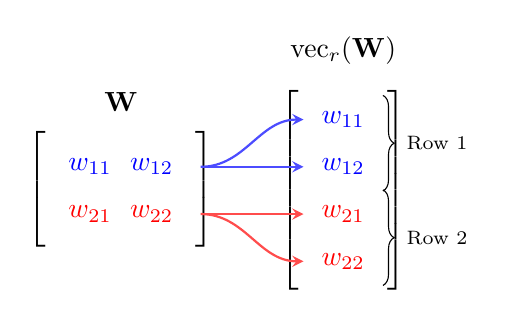
\begin{tikzpicture}[
            >=stealth, % Built-in arrow tip (no extra library)
            matrix_node/.style={
                matrix of math nodes,
                % ⚠️ CRITICAL: REMOVED 'ampersand replacement=\&' ⚠️
                left delimiter={[},
                right delimiter={]},
                nodes={minimum size=6mm, anchor=center}
            },
            arrow_style/.style={->, thick}
        ]
        % Matrix W
        \matrix (W) [matrix_node] {
            \textcolor{blue}{w_{11}} & \textcolor{blue}{w_{12}} \\
            \textcolor{red}{w_{21}} & \textcolor{red}{w_{22}} \\
        };
        \node[above=0.15cm of W] {$\mathbf{W}$};

        % Vector vec_r(W)
        \matrix (vecW) [matrix_node, right=1.4cm of W] {
            \textcolor{blue}{w_{11}} \\
            \textcolor{blue}{w_{12}} \\
            \textcolor{red}{w_{21}} \\
            \textcolor{red}{w_{22}} \\
        };
        \node[above=0.15cm of vecW] {$\mathrm{vec}_r(\mathbf{W})$};

        % Straight arrows (no curved paths = no errors)
        % \draw[arrow_style, blue!70] ([xshift=1pt]W-1-1.east) -- ([xshift=-2pt]vecW-1-1.west);
        % \draw[arrow_style, blue!70] ([xshift=1pt]W-1-2.east) -- ([xshift=-2pt]vecW-2-1.west);
        % \draw[arrow_style, red!70]  ([xshift=1pt]W-2-1.east) -- ([xshift=-2pt]vecW-3-1.west);
        % \draw[arrow_style, red!70]  ([xshift=1pt]W-2-2.east) -- ([xshift=-2pt]vecW-4-1.west);
        % Broken in the middle
%         \draw[arrow_style, blue!70] ([xshift=3pt]W.east |- W-1-1.center) -- ++(0.4,0) |- ([xshift=-3pt]vecW-1-1.west);
% \draw[arrow_style, blue!70] ([xshift=3pt]W.east |- W-1-1.center) -- ++(0.4,0) |- ([xshift=-3pt]vecW-2-1.west);
% \draw[arrow_style, red!70]  ([xshift=3pt]W.east |- W-2-1.center) -- ++(0.4,0) |- ([xshift=-3pt]vecW-3-1.west);
% \draw[arrow_style, red!70]  ([xshift=3pt]W.east |- W-2-1.center) -- ++(0.4,0) |- ([xshift=-3pt]vecW-4-1.west);
        \draw[arrow_style, blue!70] ([xshift=3pt]W.east |- W-1-1.center) to[out=0,in=180] ([xshift=-3pt]vecW-1-1.west);
        \draw[arrow_style, blue!70] ([xshift=3pt]W.east |- W-1-1.center) to[out=0,in=180] ([xshift=-3pt]vecW-2-1.west);
        \draw[arrow_style, red!70]  ([xshift=3pt]W.east |- W-2-1.center) to[out=0,in=180] ([xshift=-3pt]vecW-3-1.west);
        \draw[arrow_style, red!70]  ([xshift=3pt]W.east |- W-2-1.center) to[out=0,in=180] ([xshift=-3pt]vecW-4-1.west);
        % Braces
        \draw[decorate, decoration={brace, amplitude=4pt}] 
            ([xshift=3pt]vecW-1-1.north east) -- ([xshift=3pt]vecW-2-1.south east)
            node[midway, right=5pt, font=\scriptsize] {Row 1};
        \draw[decorate, decoration={brace, amplitude=4pt}] 
            ([xshift=3pt]vecW-3-1.north east) -- ([xshift=3pt]vecW-4-1.south east)
            node[midway, right=5pt, font=\scriptsize] {Row 2};
        \end{tikzpicture}
        \par\smallskip
        (a) Row-wise vectorization
    \end{minipage}
    \hfill % ← CRITICAL: forces left/right separation
    % RIGHT: Table (47% width)
    \begin{minipage}[c]{0.47\textwidth}
        \centering
        \small
        \renewcommand{\arraystretch}{1.3}
        \begin{tabular}{ll}
            \toprule
            \textbf{Object} & \textbf{Dimension} \\
            \midrule
            $\mathbf{F}$ & $n \times d$ \\
            $\mathrm{vec}_r(\mathbf{F})$ & $nd \times 1$ \\
            $\mathrm{vec}_r(\mathbf{W}_i)$ & $p_i q_i \times 1$ \\
            \midrule
            Jacobian $\frac{\partial \mathbf{F}}{\partial \mathbf{W}_i}$ & $nd \times p_i q_i$ \\
            Hessian $\frac{\partial^2 \mathbf{F}}{\partial \mathbf{W}_i \partial \mathbf{W}_j}$ & $(nd \cdot p_i q_i) \times p_j q_j$ \\
            \bottomrule
        \end{tabular}
        \par\smallskip
        (b) Dimensionality scheme
    \end{minipage}
    
    \vspace{0.4cm}
    \caption{\textbf{Notational preliminaries.} (a) Row-wise vectorization $\mathrm{vec}_r(\cdot)$. (b) Dimensionality of derivatives for weights $\mathbf{W}_i \in \mathbb{R}^{p_i \times q_i}$.}
    \label{fig:prelim_concepts}
\end{figure}

\subsection{Matrix Calculus and Dimensions}
We consider matrix-valued functions \(\mathbf{F}: \mathbb{R}^{p \times q} \to \mathbb{R}^{n \times d}\). Determining the dimensions of derivatives for such functions requires systematic unfolding. We verify dimensions using the layout convention where the derivative of a vector with respect to a transposed vector yields the Jacobian matrix.

Let \(\mathbf{W}_i \in \mathbb{R}^{p_i \times q_i}\) and \(\mathbf{W}_j \in \mathbb{R}^{p_j \times q_j}\) be weight matrices. The first-order derivative (Jacobian) and the second-order derivative (Hessian Block) are defined via vectorization as follows:
\begin{equation}
    \frac{\partial \mathbf{F}}{\partial \mathbf{W}_i} := \frac{\partial \mathrm{vec}_r(\mathbf{F})}{\partial \mathrm{vec}_r(\mathbf{W}_i)^\top}, \quad 
    \frac{\partial^2 \mathbf{F}}{\partial \mathbf{W}_i \partial \mathbf{W}_j} := \frac{\partial \mathrm{vec}_r\left(\frac{\partial \mathbf{F}}{\partial \mathbf{W}_i}\right)}{\partial \mathrm{vec}_r(\mathbf{W}_j)^\top}.
\end{equation}
The dimensional analysis of these objects is summarized in Figure~\ref{fig:prelim_concepts}(b). 

\subsection{Hessian Decomposition for Composite Functions}

We consider an arbitrary, twice-differentiable scalar loss function \(\mathcal{L}: \mathbb{R}^{L \times d_V} \to \mathbb{R}\), which maps the network output to a scalar value (e.g., Mean Squared Error or Cross-Entropy). The optimization objective is the composite function \(\mathcal{J}(\mathbf{w}) = \mathcal{L}(\mathbf{F}(\mathbf{X}; \mathbf{w}))\). To analyze the curvature of \(\mathcal{J}\) with respect to parameter matrices \(\mathbf{W}_i \in \mathbb{R}^{p_i \times q_i}\) and \(\mathbf{W}_j \in \mathbb{R}^{p_j \times q_j}\), we utilize the Gauss-Newton decomposition \citep{schraudolph2002aproxhessian}, following which we obtain the $(i,j)$-th block of the full Hessian $\mathbf{H}$:

\begin{equation} \label{eq:gauss_decomposition}
\frac{\partial^2 (\mathcal{L} \circ \mathbf{F})}{\partial \mathbf{W}_i \partial \mathbf{W}_j} = 
\underbrace{\left(\frac{\partial \mathbf{F}}{\partial \mathbf{W}_i}\right)^\top \frac{\partial^2 \mathcal{L}}{\partial \mathbf{F}^2} \left(\frac{\partial \mathbf{F}}{\partial \mathbf{W}_j}\right)}_{\textbf{Outer Term}} 
+ 
\underbrace{\left( \frac{\partial \mathcal{L}}{\partial \mathbf{F}} \otimes \mathbf{I}_{p_i q_i} \right) \frac{\partial^2 \mathbf{F}}{\partial \mathbf{W}_i \partial \mathbf{W}_j}}_{\textbf{Functional Term}}
\end{equation}

\noindent This decomposition holds for any twice-differentiable composite function. The terms have distinct geometric interpretations:

\textbf{The Outer Term:} This component captures the curvature induced by the loss function $\mathcal{L}$ projected onto the parameter space via the first-order Jacobians of the model. In the neighborhood of a stationary point (where $\nabla \mathcal{L} \to 0$) or in linear models, this term dominates \citep{martens2020kfac}. It is symmetric and Positive Semi-Definite if the loss $\mathcal{L}$ is convex with respect to its inputs $\mathbf{F}$ \citep{boyd2004convex}.
    
\textbf{The Functional Term:} This component involves the gradient of the loss $\frac{\partial \mathcal{L}}{\partial \mathbf{F}}$, contracting with the model's Hessian. For highly non-linear architectures like Transformers, specifically due to LayerNorm and Softmax operations, this term is non-trivial and often breaks the convex property of the total Hessian \citep{dauphin2014computationalcomplexity}.

In the subsequent sections, we derive analytic expressions for $\frac{\partial^2 \mathbf{F}}{\partial \mathbf{W}_i \partial \mathbf{W}_j}$.

% Let \(f_{\mathbf{w}}(\cdot)\) denote a neural network (here, a Self-Attention layer or full Transformer block) with parameters \(\mathbf{w} \in \Omega\). Given a twice-differentiable loss \(l(\cdot, \cdot)\), the per-sample loss is \(l_i(\mathbf{w}) := l(f_{\mathbf{w}}(\mathbf{x}_i), \mathbf{y}_i)\). The empirical loss over \( L = k\) samples is \(\mathcal{L}_k(\mathbf{w}) = \frac{1}{k} \sum_{i=1}^k l_i(\mathbf{w})\), with Hessian \(\mathbf{H}^{(k)}(\mathbf{w}) = \frac{1}{k} \sum_{i=1}^k \nabla^2_{\mathbf{w}} l_i(\mathbf{w})\).

% \begin{assumption} \label{as:zero_grad}
% At local minimum \(\mathbf{w}^*\), \(\nabla \mathcal{L}_{k-1}(\mathbf{w}^*) = \nabla \mathcal{L}_k(\mathbf{w}^*) = 0\).
% \end{assumption}
% Our study on the feasibility of this assumption is in Appendix \ref{app:exp_assumption_check}.

\section{Transformer-block Decomposition} \label{sec:method}
\begin{wrapfigure}{r}{0.3\textwidth}
\centering
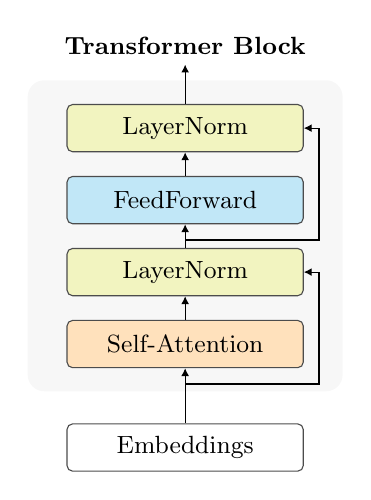
\begin{tikzpicture}[
      font=\small,
      >={Latex[length=1mm,width=1mm]},
      layer/.style={rounded corners=2pt, draw=black!70, minimum width=3cm, minimum height=6mm, align=center},
      layernorm/.style={layer, fill=ln},
      selfattn/.style={layer, fill=sa},
      feedforward/.style={layer, fill=ff},
]

\node[rounded corners=6pt, minimum width=40mm, minimum height=39.5mm, fill=black!3, anchor=north west] (transformer_block) {};
\node[above=2mm of transformer_block.north] (title) {\textbf{Transformer Block}};

\node[layer, below=4mm of transformer_block.south, anchor=north] (emb) {Embeddings};
\node[selfattn, above=3mm of transformer_block.south] (sa) {Self-Attention};
\node[layernorm, above=3mm of sa] (ln1) {LayerNorm};
\coordinate (sa_south_east) at ($(sa.south)+(17mm,-2mm)$);

\draw[->] (emb.north) -- (sa.south);
\draw[->] (sa.north) -- (ln1.south);
\draw[->] ($(sa.south)+(0mm,-2mm)$) -- (sa_south_east) |- ($(ln1.east)+(0mm,0mm)$);

\node[feedforward, above=3mm of ln1] (ff) {FeedForward};
\node[layernorm, above=3mm of ff] (ln2) {LayerNorm};
\coordinate (ff_south_east) at ($(ff.south)+(17mm,-2mm)$);

\draw[->] (ln1.north) -- (ff.south);
\draw[->] (ff.north) -- (ln2.south);
\draw[->] (ln2.north) -- ($(ln2.north)+(0mm,5mm)$);
\draw[->] ($(ff.south)+(0mm,-2mm)$) -- (ff_south_east) |- ($(ln2.east)+(0mm,0mm)$);

% \node[above=1mm of transformer_block.north west] {$L\times$};

\end{tikzpicture}
\caption{Schematic of the standard Post-Norm Transformer block architecture analyzed in this work.}
\label{fig:transformer}
\end{wrapfigure}

To systematically derive the full Hessian, we first formally define the components of the Transformer block used in our analysis. We consider a standard single-head attention block with post-layer normalization, as depicted in Figure~\ref{fig:transformer}.

Let the input sequence of generic embeddings be \(\mathbf{X} \in \mathbb{R}^{L \times d_V}\). The core mechanism is the Self-Attention (SA) layer, defined as:
\begin{equation} \label{eq:self_attention}
    \mathrm{SA}(\mathbf{X}) = \mathbf{A}(\mathbf{X}) \mathbf{X} \mathbf{W}_V,
\end{equation}
where the attention probability matrix \(\mathbf{A}(\mathbf{X})\) is governed by the query and key projections:
\[
\mathbf{A}(\mathbf{X}) = \mathrm{softmax}\left( \frac{\mathbf{X} \mathbf{W}_Q \mathbf{W}_K^\top \mathbf{X}^\top}{\sqrt{d_K}} \right).
\]
Here, the weight matrices are \(\mathbf{W}_Q, \mathbf{W}_K \in \mathbb{R}^{d_V \times d_K}\) and \(\mathbf{W}_V \in \mathbb{R}^{d_V \times d_V}\).

The full Transformer block integrates this mechanism with residual connections, Layer Normalization, and a Feed-Forward Network. We formalize the block as a composite function of recursive updates. First, the attention output is added to the residual stream and normalized:
\begin{align}
    \mathbf{Y} &= \text{LayerNorm}\Big(\mathbf{X} + \mathrm{SA}(\mathbf{X})\Big). \label{eq:transformer_mid}
\end{align}
Subsequently, this intermediate representation $\mathbf{Y}$ flows through a non-linear Feed-Forward Network ($\mathrm{FFN}$) and a second normalization step to produce the final block output $\mathbf{Z}$:
\begin{align}
    \mathbf{Z} &= \text{LayerNorm}\Big(\mathbf{Y} + \mathrm{FFN}(\mathbf{Y})\Big). \label{eq:transformer}
\end{align}
The $\mathrm{FFN}(\cdot)$ typically consists of two linear transformations separated by a non-linear activation (e.g., ReLU or GELU). The Layer Normalization operation for an arbitrary input $\mathbf{U} \in \mathbb{R}^{m \times n}$ is defined row-wise:
\begin{align} \label{eq:layer_norm}
\text{LayerNorm}(\mathbf{U})_{i,j} = \boldsymbol{\gamma}_j \frac{\mathbf{U}_{i,j} - \mu_i}{\sqrt{\sigma_i^2}} + \boldsymbol{\beta}_j,
\end{align}
where $\mu_i$ and $\sigma_i^2$ are the mean and variance of the $i$-th row. For the sake of Hessian simplicity, we treat the affine parameters $\boldsymbol{\gamma}, \boldsymbol{\beta}$ as constants in our derivation, focusing on the curvature induced by the weight matrices $\mathbf{W}$.

% Consider input embeddings \(\mathbf{X} \in \mathbb{R}^{L \times d_V}\). A single-head Self-Attention layer outputs
% \begin{equation} \label{eq:self_attention}
%     \mathrm{SA}(\mathbf{X}) = \mathbf{A}(\mathbf{X}) \mathbf{X} \mathbf{W}_V,
% \end{equation}
% where \(\mathbf{A}(\mathbf{X}) = \mathrm{softmax}\left( \frac{\mathbf{X} \mathbf{W}_Q \mathbf{W}_K^\top \mathbf{X}^\top}{\sqrt{d_K}} \right)\), and \(\mathbf{W}_Q, \mathbf{W}_K \in \mathbb{R}^{d_V \times d_K}\), \(\mathbf{W}_V \in \mathbb{R}^{d_V \times d_V}\). 

% Full Transformer block is:
% \begin{align}
% \text{LayerNorm}\Big(\mathbf{\text{LayerNorm}(\mathbf{X} + \mathrm{SA}(\mathbf{X}))} + \mathrm{FFN}(\mathbf{\text{LayerNorm}(\mathbf{X} + \mathrm{SA}(\mathbf{X}))})\Big)
% \end{align}
% where \(\mathrm{FFN}(\cdot)\) is a fully connected block with a non-linear activation within it. LayerNorm for an input matrix $\mathbf{U} \in \mathbb{R}^{m \times n}$ is \(\text{LayerNorm}(\mathbf{U})_{i,j} = \gamma_j \frac{\mathbf{U}_{i,j} - \mu_i}{\sqrt{\sigma_i^2}} + \mathbf{\beta}_j\), where $\mu_i = \frac{1}{m} \sum_{j=1}^m \mathbf{U}_{i,j}, \quad \sigma_i^2 = \frac{1}{m} \sum_{j=1}^m (\mathbf{U}_{i,j} - \mu_i)^2$. More details on a transformer block are in Section \ref{subsec:hessian_transformer_block}.
% \begin{assumption} \label{as:non_zero_variance}
% For input matrices to LayerNorm (e.g., \(\mathbf{X} + \mathrm{SA}(\mathbf{X})\), \(\mathbf{Y} + \mathrm{FFN}(\mathbf{Y})\)), the per-row variances satisfy \(\min_i \sigma_i^2 > 0\).
% \end{assumption}
% It's a technical assumption for the proof part simplification and numerical stability. The same effect can be achieved by adding some positive constant to the denominator, but it makes calculations harder. In our case this assumption is required for $\mathbf{X} + \mathrm{SA}(\mathbf{X})$ and $\mathbf{Y} + \text{FFN}(\mathbf{Y})$, defined in Transformer block \ref{eq:transformer}.

% ====================================================================================================================


\subsection{Self-Attention}\label{subsec:hessian_self_attention}

We start our analysis in the properties of the isolated Self-Attention (SA) mechanism. Following the foundational derivation from \citep{ormaniec2024attentionhessian}, the Hessian of the loss with respect to attention parameter blocks $\mathbf{W}_i, \mathbf{W}_j \in \{\mathbf{W}_Q, \mathbf{W}_K, \mathbf{W}_V\}$ admits the Gauss-Newton decomposition:
\[
\mathbf{H}(\mathbf{W}_i, \mathbf{W}_j) = 
\mathbf{H}_o(\mathbf{W}_i, \mathbf{W}_j) + \mathbf{H}_f(\mathbf{W}_i, \mathbf{W}_j).
\]
While prior works \citep{ormaniec2024attentionhessian, noci2022signalpropagationtransformerstheoretical}, primarily scrutinized this structure under the assumption of Mean Squared Error (MSE) loss, we observe that the expressions for the Jacobian and second-order kinematic derivatives derived in prior work remain valid for arbitrary twice-differentiable objectives, such as Cross-Entropy, provided the outer loss derivatives are substituted appropriately, which we utilize in our consequent analysis of the full Transformer block.

% We start our full transformer analysis with the result from \textcolor{red}{REF: Ormaniec paper} for Self-Attention part, which can be decomposed using the Gauss-Newton approximation \ref{eq:gauss_decomposition}:
% \[
% \mathbf{H}_k(\mathbf{W}_i, \mathbf{W_j}) = \frac{\partial^2 l}{\partial \mathbf{W}_i \partial \mathbf{W}_j} = \mathbf{H}_o(\mathbf{W}_i, \mathbf{W}_j) + \mathbf{H}_f(\mathbf{W}_i, \mathbf{W}_j),
% \]
% with \(\mathbf{H}_o\) as the outer-product Hessian and \(\mathbf{H}_f\) as the functional Hessian. The results for this decomposition  \textcolor{red}{write for an arbitrary Loss function (or mb say that we remark that the result can be easily generalized for an arbitrary Loss function, in particular Cross-Entropy, which is more suitable for LLM training) can be calculated according to Theorems 3.1-3.2} from \citep{ormaniec2024attentionhessian}.

\textbf{Hessian's norm estimation}

Next, we introduce a theorem for estimation the spectral norm (Definition \ref{def:matrix_norms}) of the Hessian for a single Self-Attention block.

% \begin{theorem}\label{thm:self_attention_hessian_estimation}

% Let \(\|\cdot\|_2\) be a spectral matrix norm, then for a single Self-Attention layer we have

% \[
% \|\mathbf{H}_i(\mathbf{w})\|_2 \leq M
% \]
% where
% \begin{align*}
% &M = 3\max \Bigg(\frac{2L}{d_V} \| \mathbf{X}\|^2_2, \\
%     &\quad \frac{8}{L^3 d_V d_K} \| \mathbf{W}_K\|_2^2 \| \mathbf{W}_V\|^2_2 \| \mathbf{X}\|^6_2 + \frac{12}{d_V d_K} \sqrt{\min(L, d_V)} (L \|\mathbf{X}\|_2 \|\mathbf{W}_V \|_2 + \|\textbf{Target}\|_2) \| \mathbf{W}_V \|_2 \| \mathbf{W}_K\|^2_2 \| \mathbf{X}\|^5_2, \\
%     &\quad \frac{4}{L d_V \sqrt{d_K}} \| \mathbf{W}_V\|_2 \| \mathbf{W}_K \|_2 \| \mathbf{X}\|^4_2 + \frac{4\sqrt{\min(L, d_V)}}{L^2\sqrt{d_K}} (L \|\mathbf{X}\|_2 \|\mathbf{W}_V \|_2 + \|\textbf{Target}\|_2) \|\mathbf{W}_K\|_2 \|\mathbf{X}\|^3_2,\\
%     &\quad \frac{8}{L^3 d_V d_K} \|\mathbf{W}_K\|_2 \|\mathbf{W}_Q\|_2 \| \mathbf{W}_V\|^2_2 \|\mathbf{X} \|^6_2 + \\
%     &+\frac{4\sqrt{\min(L, d_V)} (L \|\mathbf{X}\|_2 \|\mathbf{W}_V \|_2 + \|\textbf{Target}\|_2)}{L d_V \sqrt{d_K}} \|\mathbf{W}_V\|_2 \Big(3L \|\mathbf{W}_K\|_2 \|\mathbf{W}_Q\|_2 \| \mathbf{X}\|^5_2 + \frac{d_V}{L} \|\mathbf{X}\|^3_2\Big)\Bigg)
% \end{align*}

% The proof is provided in Appendix~\ref{app:proof_self_attention_hessian_estimation}.
% \end{theorem}

\begin{theorem}\label{thm:self_attention_hessian_estimation}
Consider a single-head Self-Attention map
$\mathrm{SA}(\mathbf X)=\mathbf A(\mathbf X)\mathbf X\mathbf W_V$ with
$\mathbf A(\mathbf X)=\mathrm{softmax}\!\big(\mathbf X\mathbf W_Q\mathbf W_K^\top \mathbf X^\top/\sqrt{d_K}\big)$,
and an arbitrary twice-differentiable loss $\mathcal L$.
Let $\mathbf H^{(i,j)}$ denote the $(i,j)$-block of the loss Hessian w.r.t.
$\mathbf W_i,\mathbf W_j\in\{\mathbf W_Q,\mathbf W_K,\mathbf W_V\}$.
Then each block admits the Gauss--Newton decomposition
\[
\mathbf H^{(i,j)}=\mathbf H_o^{(i,j)}+\mathbf H_f^{(i,j)},
\]
and its spectral norm is bounded as
\[
\|\mathbf H^{(i,j)}\|_2 \le \|\mathbf H_o^{(i,j)}\|_2+\|\mathbf H_f^{(i,j)}\|_2
\le C_o^{(i,j)} + C_f^{(i,j)}.
\]
Moreover, up to multiplicative factors depending only on
$\|\mathbf W_Q\|_2,\|\mathbf W_K\|_2,\|\mathbf W_V\|_2$, $d_V$, $d_K$
(and on outer loss derivatives), the blocks scale with the input norm as

\[
\begin{array}{c|ccc}
 & Q & K & V \\ \hline
Q & \mathcal O(\|\mathbf X\|_2^{6}) & \mathcal O(\|\mathbf X\|_2^{6}) & \mathcal O(\|\mathbf X\|_2^{5}) \\
K & \cdot                         & \mathcal O(\|\mathbf X\|_2^{6}) & \mathcal O(\|\mathbf X\|_2^{5}) \\
V & \cdot                         & \cdot                         & \mathcal O(\|\mathbf X\|_2^{4})
\end{array}
\]
and the leading functional terms are damped by $\mathcal O(L^{-3})$. In particular, the full self-attention Hessian satisfies
\[
\|\mathbf H\|_2 \le 3 \cdot \max_{i,j\in\{Q,K,V\}}\big(C_o^{(i,j)}+C_f^{(i,j)}\big),
\]
where explicit constants $C_o^{(i,j)},C_f^{(i,j)}$ are given in
Appendix~\ref{app:proof_self_attention_hessian_estimation}.
\end{theorem}

\textbf{Asymptotic Analysis.}

The bound $M$ reveals critical scaling properties of the optimization landscape. 

 \textbf{Input Sensitivity:} The bound is dominated by terms scaling as $\mathcal{O}(\|\mathbf{X}\|_2^6)$. This extreme sensitivity suggests that pre-LayerNorm placement (controlling $\|\mathbf{X}\|_2$ before attention) is crucial for stabilizing curvature, aligning with empirical observations in \citep{xiong2020prelayernorm}.

 \textbf{Sequence Length:} Several terms scale inversely with sequence length (e.g., $1/L^3$), a consequence of the softmax normalization factor. This implies that for very long sequences, the intrinsic curvature of the attention mechanism (specifically the softmax derivative contribution) may naturally dampen, potentially aiding stability in large-context training.

 

\subsection{LayerNorm}\label{subsec:layer_norm}

As defined in Eq. (\ref{eq:layer_norm}), Layer Normalization operates row-wise. To facilitate the derivation of second-order properties and ensure compatibility with the matrix calculus properties established in Appendix~\ref{app:properties}, we first reformulated this operation in compact matrix notation.

Let $\mathbf{X} \in \mathbb{R}^{L \times d_V}$. We define the centering operator $\mathbf{M}(\mathbf{X})$ and the inverse-standard-deviation operator $\mathbf{P}(\mathbf{X})$ as:
\[
\mathbf{M}(\mathbf{X}) = \mathbf{X} - \tfrac{1}{d_V}\mathbf{X}\mathbf{1}_{d_V}\mathbf{1}_{d_V}^\top, \quad
\sigma(\mathbf{X}) = \tfrac{1}{\sqrt{d_V}}\big(\mathbf{M}(\mathbf{X})^{\circ 2}\mathbf{1}_{d_V}\big)^{\circ 1/2}, \quad
\mathbf{P}(\mathbf{X}) = \mathrm{diag}^{-1}(\sigma(\mathbf{X})).
\]
Consequently, the LayerNorm operation (excluding affine parameters $\boldsymbol{\gamma}, \boldsymbol{\beta}$ which are treated as constants for the curvature analysis of weights) can be written as:
\[
\text{LayerNorm}(\mathbf{X}) = \mathbf{P}(\mathbf{X}) \mathbf{M}(\mathbf{X}).
\]

\begin{assumption} \label{as:non_zero_variance}
For all input matrices to LayerNorm, the per-row variances satisfy $\min_i \sigma_i^2 > 0$ to ensure differentiability.
\end{assumption}

We note that it's a technical assumption for the proof part simplification and numerical stability. The same effect can be achieved by adding some positive constant to the denominator, but it makes calculations less clear. We now derive the exact Jacobian and Hessian of this operator.

\begin{theorem} [Jacobian of LayerNorm] \label{thm:layernorm_derivative}
The Jacobian of $\text{LayerNorm}(\mathbf{X})$ with respect to $\mathbf{X}$ is given by:
\[
\frac{\partial \,\text{LayerNorm}(\mathbf{X})}{\partial \mathbf{X}}
= (\mathbf{P}(\mathbf{X}) \otimes \mathbf{I}_{d_V})\mathbf{G}
+ (\mathbf{I}_L \otimes \mathbf{M}(\mathbf{X})^\top) \frac{\partial \mathbf{P}(\mathbf{X})}{\partial \mathbf{X}},
\]
where $\mathbf{G} = \frac{\partial \mathbf{M}}{\partial \mathbf{X}} = \mathbf{I}_{Ld_V} - \tfrac{1}{d_V}(\mathbf{I}_L \otimes \mathbf{1}_{d_V \times d_V})$ is the constant centering projection.
The derivative of the inverse deviation $\mathbf{P}$ is:
\[
\frac{\partial \mathbf{P}}{\partial \mathbf{X}}
= \tfrac{1}{\sqrt{d_V}}
\Big( -\mathbf{D}^{-1} \otimes \mathbf{D}^{-\top} \Big)
\mathbf{E}_{diag}
\Big( 
\mathrm{diag}^{-1}\!\big(\mathrm{vec}_r^{1/2}(\mathbf{M}^{\circ 2}\mathbf{1}_{d_V})\big)
(\mathbf{I}_L \otimes \mathbf{1}_{d_V}^\top)
\mathrm{diag}(\mathrm{vec}_r(\mathbf{M}))
\mathbf{G}
\Big),
\]
with $\mathbf{D} = \mathrm{diag}(\sigma(\mathbf{X}))$ and $\mathbf{E}_{diag} = \big( \mathbf{e}_1 \otimes \mathbf{e}_1, \dots, \mathbf{e}_L \otimes \mathbf{e}_L \big)$ representing the derivative of the diagonal operator.
\end{theorem}

\begin{theorem} [Hessian of LayerNorm] \label{thm:layernorm_second_derivative} The Hessian $\frac{\partial^2 \text{LayerNorm}}{\partial \mathbf{X}^2}$ is given by the derivative of the Jacobian terms:
\begin{align*}
\frac{\partial^2 \text{LayerNorm}}{\partial \mathbf{X}^2} &= 
\left( \mathbf{I}_{L d_V} \otimes \mathbf{G}^\top \right) \frac{\partial (\mathbf{P}(\mathbf{X}) \otimes \mathbf{I}_{d_V})}{\partial \mathbf{X}} \\
&+ \left( (\mathbf{I}_L \otimes \mathbf{M}^\top ) \otimes \mathbf{I}_{L d_V} \right) \frac{\partial^2 \mathbf{P}}{\partial \mathbf{X}^2} + \left( \mathbf{I}_{L d_V} \otimes  \left(\frac{\partial \mathbf{P}}{\partial \mathbf{X}}\right)^\top \right) \frac{\partial (\mathbf{I}_L \otimes \mathbf{M}^\top )}{\partial\mathbf{X}}.
\end{align*}
Note that the term involving $\frac{\partial^2 \mathbf{M}}{\partial \mathbf{X}^2}$ vanishes because the centering operation is linear. Explicit forms for the remaining second-order terms are derived in the proof.
\end{theorem}

The detailed proofs for Theorems \ref{thm:layernorm_derivative} and \ref{thm:layernorm_second_derivative} rely on the expansion of Kronecker derivative properties and are provided in Appendices~\ref{app:proof_layernorm_derivative} and \ref{app:proof_layernorm_second_derivative}.



\subsection{Feed-Forward Network} \label{subsec:ffn}

The Feed-Forward Network (FFN) introduces essential non-linearity into the Transformer block. While some prior theoretical works allow for linear approximations of the FFN to simplify signal propagation analysis \citep{noci2022signalpropagationtransformerstheoretical}, we explicitly model the standard non-linear formulation:
\[
\mathrm{FFN}(\mathbf{Y}) = \sigma(\mathbf{Y}\mathbf{W}_1)\mathbf{W}_2,
\]
where $\mathbf{W}_1 \in \mathbb{R}^{d_V \times d_{ff}}$, $\mathbf{W}_2 \in \mathbb{R}^{d_{ff} \times d_V}$, and $\sigma(\cdot) = \mathrm{ReLU}(\cdot)$. To handle the non-differentiability of ReLU at zero, we utilize the following lemma.

\begin{lemma}[ReLU Jacobian and Hessian] \label{lemma:relu_derivative_hessian}
Let $\mathbf{X} \in \mathbb{R}^{m \times n}$. The element-wise $\mathrm{ReLU}$ is differentiable almost everywhere. Its Jacobian and Hessian with respect to the input $\mathbf{X}$ are given by:
\[ 
\frac{\partial \mathrm{ReLU}(\mathbf{X})}{\partial \mathbf{X}} = \mathbf{D}_\sigma(\mathbf{X}) := \mathrm{diag}\!\big(\mathrm{vec}_r(\mathbf{1}_{\{\mathbf{X}>0\}})\big), \quad \text{and} \quad \frac{\partial^2 \mathrm{ReLU}(\mathbf{X})}{\partial \mathbf{X}^2} = \mathbf{0}. 
\]
\end{lemma}
\begin{proof}
See Appendix \ref{app:additional_properties}.
\end{proof}

Using this result, we determine the exact first-order derivatives ($\mathbf{B}_i$ terms) needed for the functional Hessian in Eq.~(\ref{eq:gauss_decomposition}).

\begin{proposition}[FFN Jacobians] \label{prop:ffn_jacobians}
Let $\mathbf{Z} = \sigma(\mathbf{Y}\mathbf{W}_1)\mathbf{W}_2$. The Jacobians with respect to the weights are:
\begin{align}
    \frac{\partial \mathbf{Z}}{\partial \mathbf{W}_2} &= \sigma(\mathbf{Y}\mathbf{W}_1) \otimes \mathbf{I}_{d_V}, \label{eq:ffn_jac_w2} \\
    \frac{\partial \mathbf{Z}}{\partial \mathbf{W}_1} &= (\mathbf{I}_L \otimes \mathbf{W}_2^\top)\, \mathbf{D}_\sigma\, (\mathbf{Y} \otimes \mathbf{I}_{d_{ff}}), \label{eq:ffn_jac_w1}
\end{align}
where $\mathbf{D}_\sigma = \mathrm{diag}(\mathrm{vec}_r(\mathbf{1}_{\{\mathbf{Y}\mathbf{W}_1 > 0\}}))$.
\end{proposition}

\begin{proof}
We apply the vectorization properties from Appendix~\ref{app:properties}. For $\mathbf{W}_2$, the function is of the linear form $\mathbf{A} \mathbf{W}_2 \mathbf{B}$ with $\mathbf{A} = \sigma(\mathbf{Y}\mathbf{W}_1)$ and constant $\mathbf{B} = \mathbf{I}_{d_V}$. A direct application of the Matrix-Product Derivative (Property~\ref{prop:matrix_product_derivative}) yields first result. For $\mathbf{W}_1$, we apply the chain rule through the activation function. The gradient of the output with respect to the post-activation matrix is $\mathbf{I}_L \otimes \mathbf{W}_2^\top$ by Property~\ref{prop:matrix_product_derivative}. The gradient of the activation is $\mathbf{D}_\sigma$ by Lemma~\ref{lemma:relu_derivative_hessian}. Finally, the gradient of the pre-activation $ \mathbf{Y}\mathbf{W}_1\mathbf{I}_{d_{ff}} $ with respect to the weights is $\mathbf{Y} \otimes \mathbf{I}_{d_{ff}}$. Multiplying these three Jacobian matrices yields the second result.
\end{proof}

\begin{figure}[t]
    \centering
    % LEFT PANEL
    \begin{minipage}[t]{0.48\textwidth}
        \centering
        \includegraphics[width=\linewidth]{figs/hessian_entries.pdf}
        \caption{Hessian entries for an \textbf{initialized model}. Note the magnitude heterogeneity; the \textcolor{olive}{Values} corresponding blocks have larger values.}
        \label{fig:hessian_entries}
    \end{minipage}
    \hfill
    % RIGHT PANEL
    \begin{minipage}[t]{0.48\textwidth}
        \centering
        \includegraphics[width=\linewidth]{figs/hessian_entries_trained.pdf}
        \caption{Hessian entries after \textbf{training} for several epochs. While magnitudes increase, the \textcolor{olive}{Values-Values} blocks remain the high-curvature dominant terms.}
        \label{fig:hessian_entries_trained}
    \end{minipage}
    \label{fig:hessian_viz}
\end{figure}

\subsection{Full Transformer Block} \label{subsec:hessian_full}

Having characterized the differential properties of the LayerNorm operator (Section~\ref{subsec:layer_norm}) and the Feed-Forward Network (Section~\ref{subsec:ffn}), we now integrate these components with the Self-Attention mechanism to derive the full Transformer block Hessian, explicitly accounting for the Residual connections, which result mathematically as identity matrices within the Jacobian chain rule, preventing gradient collapse and distinguishing our exact derivation from simplified approximations.

Let the parameter set be $\mathbf{w} = \{\mathbf{W}_1, \mathbf{W}_2, \mathbf{W}_Q, \mathbf{W}_K, \mathbf{W}_V\}$. The block output is the composite signal defined in Eq. (\ref{eq:transformer}):
\[
\mathbf{Z} = \mathrm{LayerNorm}(\mathbf{S}), \quad \text{where} \quad \mathbf{S} = \mathbf{Y} + \mathrm{FFN}(\mathbf{Y}) \quad \text{and} \quad \mathbf{Y} = \mathrm{LayerNorm}(\mathbf{X} + \mathrm{SA}(\mathbf{X})).
\]

We first establish the first-order Jacobians, which serve as the linear operators for signal propagation.

\begin{theorem}[Transformer Block Jacobians] \label{thm:transformer_derivative}
For any weight matrix $\mathbf{W}_i \in \mathbf{w}$, the Jacobian of the output $\mathbf{Z}$ is given by the chain rule through the final LayerNorm:
\[
\frac{\partial \mathbf{Z}}{\partial \mathbf{W}_i} = \mathbf{J}_{Z} \mathbf{B}_i,
\]
where $\mathbf{J}_{Z} := \frac{\partial \mathrm{LayerNorm}(\mathbf{S})}{\partial \mathbf{S}}$ is the operator from Theorem~\ref{thm:layernorm_derivative}, and $\mathbf{B}_i := \frac{\partial \mathbf{S}}{\partial \mathbf{W}_i}$ represents the gradient flow into the final residual stream. Specifically:

1. \textbf{Feed-Forward Weights ($i \in \{1, 2\}$):} $\mathbf{B}_i$ matches the FFN Jacobians derived in Proposition \ref{prop:ffn_jacobians}:
   \begin{align*}
       \mathbf{B}_1 &= (\mathbf{I}_L \otimes \mathbf{W}_2^\top)\, \mathbf{D}_\sigma\, (\mathbf{Y} \otimes \mathbf{I}_{d_{ff}}), \\
       \mathbf{B}_2 &= \sigma(\mathbf{Y}\mathbf{W}_1) \otimes \mathbf{I}_{d_V}.
   \end{align*}

2. \textbf{Attention Weights ($i \in \{K, Q, V\}$):} The gradient flows back through the FFN residual and the first LayerNorm:
   \[
   \mathbf{B}_i = \mathbf{J}_{SY} \mathbf{J}_{Y} \mathbf{G}_i.
   \]
   Here, $\mathbf{J}_{SY} = \frac{\partial \mathbf{S}}{\partial \mathbf{Y}}$ explicitly includes the Residual Connection via the identity term:
   \[
   \mathbf{J}_{SY} = (\mathbf{I}_L \otimes \mathbf{W}_2^\top)\mathbf{D}_\sigma (\mathbf{I}_L \otimes \mathbf{W}_1^\top) + (\mathbf{I}_L \otimes \mathbf{I}_{d_V}).
   \]
   $\mathbf{J}_{Y}$ is the first LayerNorm Jacobian, and $\mathbf{G}_i$ are the Self-Attention Jacobians from \citep{noci2022signalpropagationtransformerstheoretical}.
\end{theorem}
\begin{proof}
See Appendix \ref{app:proof_transformer_derivative}. The derivation is a direct application of the chain rule using the matrix calculus properties established in Section \ref{sec:prelim}.
\end{proof}

We now state our main result: the explicit characterization of the Transformer Hessian blocks. This theorem connects the Functional Term from the Gauss-Newton decomposition (Eq. \ref{eq:gauss_decomposition}) to the specific architectural components.

\begin{theorem}[Transformer Block Hessian] \label{thm:transformer_hessian}
The Hessian block of the output $\mathbf{Z}$ with respect to parameter pair $(\mathbf{W}_i, \mathbf{W}_j)$ is:
\begin{equation} \label{eq:block_hessian_transformer}
\boxed{
\;\mathbf{H}_{\mathrm{tr}}^{(i,j)} := \frac{\partial^2 \mathbf{Z}}{\partial \mathbf{W}_i \partial \mathbf{W}_j}
= 
\underbrace{\left( \mathbf{J}_Z \otimes \mathbf{I}_{n_i} \right) \boldsymbol{\xi}_{ij}}_{\text{Inter-layer Interaction}}
  + 
\underbrace{\left( \mathbf{I}_{L d_V} \otimes \mathbf{B}_i^\top \right) \mathbf{H}_Z \mathbf{B}_j}_{\text{Normalization Curvature}}
\; } 
\end{equation}
where $\mathbf{H}_Z$ is the LayerNorm Hessian (Theorem \ref{thm:layernorm_second_derivative}) and $\boldsymbol{\xi}_{ij} := \frac{\partial \mathbf{B}_i}{\partial \mathbf{W}_j}$ captures the second-order interactions between sub-layers. The interaction terms $\boldsymbol{\xi}_{ij}$ are:

\begin{enumerate}
    \item \textbf{FFN Curvature:} Due to the piecewise-linearity of ReLU (Lemma \ref{lemma:relu_derivative_hessian}), the second derivatives $\xi_{11}$ and $\xi_{22}$ vanish almost everywhere. However, the interaction between FFN layers is non-zero (detailed in Appendix \ref{app:proof_transformer_hessian_estimate}).
    
    \item \textbf{Attention-FFN Interaction:} Cross-terms $\boldsymbol{\xi}_{1k}$ capture how attention weights scale the gradients flowing into the FFN via $\mathbf{D}_\sigma$.
    
    \item \textbf{Attention Curvature:} Terms $\boldsymbol{\xi}_{k\ell}$ incorporate the second derivatives of the softmax function $\boldsymbol{\Phi}_{k\ell}$ derived in \citep{ormaniec2024attentionhessian}, modulated by the residual path $\mathbf{J}_{SY}$.
\end{enumerate}
\end{theorem}

\textbf{Connection to the Loss Landscape.} 
Theorem \ref{thm:transformer_hessian} resolves the cryptic functional term $\frac{\partial^2 \mathbf{F}}{\partial \mathbf{W}^2}$ in the general Gauss-Newton decomposition. For a general twice-differentiable loss function $\mathcal{L}$, the full Hessian of the objective $\mathcal{J}(\mathbf{w}) = \mathcal{L}(\mathbf{Z}(\mathbf{w}))$ is:
\begin{equation} \label{eq:transformer_decomposition}
\frac{\partial^2 \mathcal{J}}{\partial \mathbf{W}_i \partial \mathbf{W}_j} 
= 
\underbrace{(\mathbf{J}_Z \mathbf{B}_i)^\top \frac{\partial^2 \mathcal{L}}{\partial \mathbf{Z}^2} (\mathbf{J}_Z \mathbf{B}_j)}_{\text{Loss Convexity}} 
+ 
\underbrace{\left( \frac{\partial \mathcal{L}}{\partial \mathbf{Z}} \otimes \mathbf{I}_{p_i q_i} \right) \mathbf{H}_{\text{tr}}^{(i,j)}}_{\text{Architectural Curvature}}.
\end{equation}
This decomposition reveals that even for a convex loss, where the first term is positively semi-defined, the optimization landscape becomes non-convex due to $\mathbf{H}_{\text{tr}}^{(i,j)}$.

Finally, we provide a computable upper bound on the curvature, essential for determining step sizes and convergence rates.

\begin{theorem}[Spectral Bounds] \label{thm:transformer_hessian_estimate}
Let $\mathbf{H}_{\mathrm{tr}}$ be the full Hessian matrix for the block, composed of $m_b \times n_b = 25$ blocks. Its spectral norm is bounded by:
\begin{equation} \label{eq:full_bound_transformer}
\|\mathbf{H}_{\mathrm{tr}}\|_2
\;\le\;
5 \cdot \max_{i,j} \left(
    \|\frac{\partial^2 \mathcal{L}}{\partial \mathbf{Z}^2}\|_2 \|\mathbf{J}_Z \mathbf{B}_i\|_2 \|\mathbf{J}_Z \mathbf{B}_j\|_2 
    + 
    \big\|\frac{\partial \mathcal{L}}{\partial \mathbf{Z}}\big\|_2 \left( \|\mathbf{J}_Z\|_2 \|\boldsymbol{\xi}_{ij}\|_2 + \|\mathbf{B}_i\|_2 \|\mathbf{H}_Z\|_2 \|\mathbf{B}_j\|_2 \right)
\right).
\end{equation}
For Mean Squared Error, $\|\frac{\partial^2 \mathcal{L}}{\partial \mathbf{Z}^2}\|_2 = \frac{2}{L d_V}$. The terms $\|\boldsymbol{\xi}_{ij}\|_2$ and $\|\mathbf{H}_Z\|_2$ are explicitly bounded by polynomials of the input norm $\|\mathbf{X}\|_2$ and weight norms in Appendix \ref{app:proof_transformer_hessian_estimate}.
\end{theorem}

At initialization (Figure~\ref{fig:hessian_entries}), the spectrum is highly anisotropic, with Value interactions clearly distinguishable from the background noise of FFN curvature. After training the model for several iterations until convergence (Figure~\ref{fig:hessian_entries_trained}), we observe that while the overall scale of the Hessian increases, the relative structural dominance of the $\mathbf{W}_V$-$\mathbf{W}_V$ block persists. This confirms that the specific polynomial scaling factors identified in Theorem~\ref{thm:self_attention_hessian_estimation} correctly predict the principal sources of curvature in the Transformer landscape. Additional layer-wise Hessians visualizations are present in Appendix \ref{app:A}.

%============================================================================================================================


% \subsection{\textcolor{red}{Transformer-block}} \label{subseq:transformer_block}

% Thus, we calculate the derivatives and the Hessian of the proposed Transformer block representation \ref{eq:transformer}.

% \begin{theorem}[Transformer block derivative] \label{thm:transformer_derivative}

% The Transformer block is defined in \ref{eq:transformer}. The derivative \(\frac{\partial\mathbf{Z}}{\partial \mathbf{W}_i}\) is calculated as follows.

% For $i \in \{1,2\}$:
% \begin{align*}
%     \frac{\partial\mathbf{Z}}{\partial \mathbf{W}_i} &= \frac{\partial \text{LayerNorm}(\text{FFN}(\mathbf{Y}) + \mathbf{Y})}{\partial (\text{FFN}(\mathbf{Y}) + \mathbf{Y})} \frac{\partial (\text{FFN}(\mathbf{Y}) + \mathbf{Y})}{\partial \mathbf{W}_i},
% \end{align*}
% where
% \begin{equation*}
%     \frac{\partial (\text{FFN}(\mathbf{Y}) + \mathbf{Y})}{\partial \mathbf{W}_i} = \begin{cases}
%         \left(\mathbf{I}_L \otimes \mathbf{W}_2^\top \right) \mathrm{diag}\!\big(\mathrm{vec}_r(\mathbf{1}_{\{\mathbf{X}>0\}})\big) \left( \mathbf{Y} \otimes \mathbf{I}_{d_{ff}}\right), & \text{for } i = 1 \\
%         \sigma(\mathbf{Y} \mathbf{W}_1) \otimes \mathbf{I}_{d_V}, & \text{for } i = 2
%     \end{cases},
% \end{equation*}
% and \(\frac{\partial \text{LayerNorm}(\text{FFN}(\mathbf{Y}) + \mathbf{Y})}{\partial (\text{FFN}(\mathbf{Y}) + \mathbf{Y})} \) can be calculated following Theorem \ref{thm:layernorm_derivative} and is explicitly given in the proof

% For $i \in \{ K, Q, V\}$:
% \begin{align*}
%     \frac{\partial\mathbf{Z}}{\partial \mathbf{W}_i} &= \frac{\partial \text{LayerNorm}(\text{FFN}(\mathbf{Y}) + \mathbf{Y})}{\partial (\text{FFN}(\mathbf{Y}) + \mathbf{Y})} \frac{\partial (\text{FFN}(\mathbf{Y}) + \mathbf{Y})}{\partial \mathbf{Y}} \frac{\partial \mathbf{Y}}{\partial \mathbf{W}_i},
% \end{align*}
% where
% \begin{align*}
%     \frac{\partial (\text{FFN}(\mathbf{Y}) + \mathbf{Y})}{\partial \mathbf{Y}} &= \left( \mathbf{I}_L \otimes \mathbf{W}_2^\top\right) \mathrm{diag}\!\big(\mathrm{vec}_r(\mathbf{1}_{\{\mathbf{X}>0\}})\big) \left( \mathbf{I}_L \otimes \mathbf{W}_1^\top \right) + \left( \mathbf{I}_L \otimes \mathbf{I}_{d_V}\right),
% \end{align*}
% and \(\frac{\partial \mathbf{Y}}{\partial\mathbf{W}_i} = \frac{\partial \text{LayerNorm}(\mathrm{SA} (\mathbf{X}) + \mathbf{X})}{\partial (\mathrm{SA} (\mathbf{X}) + \mathbf{X})} \frac{\partial \mathrm{SA}(\mathbf{X})}{\partial \mathbf{W}_i}\), with \(\frac{\partial \mathrm{SA}(\mathbf{X})}{\partial \mathbf{W}_i}\) is calculated according to Lemma A.2 from \citep{noci2022signalpropagationtransformerstheoretical} and \(\frac{\partial \text{LayerNorm}(\mathrm{SA} (\mathbf{X}) + \mathbf{X})}{\partial (\mathrm{SA} (\mathbf{X}) + \mathbf{X})}\) is calculated according to Theorem \ref{thm:layernorm_derivative}.
% \end{theorem}


% Detailed proof can be found in Appendix \ref{app:proof_transformer_derivative}.

% % \begin{theorem}[Hessian of the Transformer block \ref{eq:transformer}]\label{thm:transformer_hessian}

% \begin{theorem}[Hessian of the Transformer block \ref{eq:transformer}]\label{thm:transformer_hessian}

% Let $\mathbf{X} \in \mathbb{R}^{L \times d_V}$, $\mathbf{Y} \in \mathbb{R}^{L \times d_V}$, $\mathbf{W}_1 \in \mathbb{R}^{d_V \times d_{ff}}$, $\mathbf{W}_2 \in \mathbb{R}^{d_{ff} \times d_V}$, $\mathbf{W}_Q, \mathbf{W}_K \in \mathbb{R}^{d_V \times d_K}$, $\mathbf{W}_V \in \mathbb{R}^{d_V \times d_V}$.
% Define
% \[\mathbf{S}(\mathbf{Y},\mathbf{W}_1,\mathbf{W}_2) = \sigma(\mathbf{Y}\mathbf{W}_1)\mathbf{W}_2 + \mathbf{Y} \in \mathbb{R}^{L \times d_V}, \qquad\mathbf{Z} = \mathrm{LayerNorm}(\mathbf{S}) \in \mathbb{R}^{L \times d_V},\]
% and abbreviate (according to  Theorems~\ref{thm:layernorm_derivative}--\ref{thm:layernorm_second_derivative}):
% \[\mathbf{J}_Z := \frac{\partial\,\mathrm{LayerNorm}(\mathbf{S})}{\partial \mathbf{S}} \in \mathbb{R}^{L d_V \times L d_V}, \quad\mathbf{H}_Z := \frac{\partial^2\,\mathrm{LayerNorm}(\mathbf{S})}{\partial \mathbf{S}^2} \in \mathbb{R}^{(L d_V)^2 \times L d_V}\]

% Let further
% \[\mathbf{D}_\sigma := \mathrm{diag}\big(\mathrm{vec}_r(\mathbf{1}_{\{\mathbf{Y}\mathbf{W}_1>0\}})\big) \in \mathbb{R}^{L d_{ff} \times L d_{ff}}\]
% from Lemma~\ref{lemma:relu_derivative_hessian}.

% Define the residual-Jacobian
% \[\mathbf{J}_{SY} := \frac{\partial \mathbf{S}}{\partial \mathbf{Y}} = (\mathbf{I}_L \otimes \mathbf{W}_2^\top)\mathbf{D}_\sigma (\mathbf{I}_L \otimes \mathbf{W}_1^\top) + (\mathbf{I}_L \otimes \mathbf{I}_{d_V}) \in \mathbb{R}^{L d_V \times L d_V},\]
% and for the first residual $\mathbf{Y} = \mathrm{LayerNorm}(\mathrm{SA}(\mathbf{X}) + \mathbf{X})$, set
% \[\mathbf{J}_Y := \frac{\partial \,\mathrm{LayerNorm}(\mathrm{SA}(\mathbf{X})+\mathbf{X})}{\partial (\mathrm{SA}(\mathbf{X})+\mathbf{X})} \in \mathbb{R}^{L d_V \times L d_V}, \quad \mathbf{H}_Y := \frac{\partial^2 \,\mathrm{LayerNorm}(\mathrm{SA}(\mathbf{X})+\mathbf{X})}{\partial (\mathrm{SA}(\mathbf{X})+\mathbf{X})^2} \in \mathbb{R}^{(L d_V)^2 \times L d_V}\]
% calculated by Theorems~\ref{thm:layernorm_derivative}--\ref{thm:layernorm_second_derivative}.

% Denote parameter sizes
% \[n_1 = d_V d_{ff},\quad n_2 = d_{ff} d_V,\quad n_Q = n_K = d_V d_K,\quad n_V = d_V^2.\]
% Let the attention-side Jacobians (from Theorem~\ref{thm:transformer_derivative}, can be calculated according to \citep{noci2022signalpropagationtransformerstheoretical}) be
% \[\mathbf{G}_V := \frac{\partial \mathrm{SA}}{\partial \mathbf{W}_V} \in \mathbb{R}^{L d_V \times n_V}, \quad\mathbf{G}_Q := \frac{\partial \mathrm{SA}}{\partial \mathbf{W}_Q} \in \mathbb{R}^{L d_V \times n_Q}, \quad\mathbf{G}_K := \frac{\partial \mathrm{SA}}{\partial \mathbf{W}_K} \in \mathbb{R}^{L d_V \times n_K}.\]

% For $i \in \{1,2\}$ and $k \in \{K,Q,V\}$, define first-layer Jacobians
% \[\mathbf{B}_1 := \frac{\partial \mathbf{S}}{\partial \mathbf{W}_1} = (\mathbf{I}_L \otimes \mathbf{W}_2^\top)\, \mathbf{D}_\sigma\, (\mathbf{Y} \otimes \mathbf{I}_{d_{ff}}) \in \mathbb{R}^{L d_V \times n_1}, \]
% \[\mathbf{B}_2 := \frac{\partial \mathbf{S}}{\partial \mathbf{W}_2} = \sigma(\mathbf{Y}\mathbf{W}_1) \otimes \mathbf{I}_{d_V} \in \mathbb{R}^{L d_V \times n_2},\]
% \[\mathbf{B}_k := \frac{\partial \mathbf{S}}{\partial \mathbf{W}_k} = \mathbf{J}_{SY}\, \mathbf{J}_Y\, \mathbf{G}_k \in \mathbb{R}^{L d_V \times n_k}.\]
% Then the Hessian blocks of the Transformer output $\mathbf{Z}$ w.r.t.\ parameters $(\mathbf{W}_i,\mathbf{W}_j)$ are
% \begin{equation} \label{eq:block_hessian_transformer}
% \boxed{
% \;\mathbf{H}_{\mathrm{tr}}^{(i,j)} := \frac{\partial^2 \mathbf{Z}}{\partial \mathbf{W}_i \partial \mathbf{W}_j}
% = \left( \mathbf{J}_Z \otimes \mathbf{I}_{n_i} \right) \boldsymbol{\xi}_{ij}
%   + \left( \mathbf{I}_{L d_V} \otimes \mathbf{B}_i^\top \right) \mathbf{H}_Z \mathbf{B}_j \; } 
% \end{equation}
% with
% \[\boldsymbol{\xi}_{ij} := \frac{\partial}{\partial \mathbf{W}_j} \left( \frac{\partial \mathbf{S}}{\partial \mathbf{W}_i} \right) \in \mathbb{R}^{(L d_V \cdot n_i) \times n_j}.\]

% The second Jacobians $\boldsymbol{\xi}_{ij}$ for all pairs $(i,j)$ are given almost everywhere by:

% 1) Pure-FFN pairs:
% \[
% \boldsymbol{\xi}_{11} = \mathbf{0}_{(L d_V \cdot n_1) \times n_1}, 
% \qquad 
% \boldsymbol{\xi}_{22} = \mathbf{0}_{(L d_V \cdot n_2) \times n_2},
% \]
% \[\boldsymbol{\xi}_{12} = \left( \mathbf{I}_L \otimes \mathbf{K}_{d_V, d_{ff}} \otimes \mathbf{I}_{d_V} \right) \left( \mathbf{I}_{L d_{ff}} \otimes \mathrm{vec}_r(\mathbf{I}_{d_V}) \right)\left( \mathbf{D}_\sigma \, (\mathbf{Y} \otimes \mathbf{I}_{d_{ff}}) \right),\]
% \[\boldsymbol{\xi}_{21} = \left( \mathbf{I}_L \otimes \mathbf{W}_2^\top \right) \mathbf{D}_\sigma \left( \mathbf{I}_L \otimes \mathbf{K}_{d_{ff}, d_V} \otimes \mathbf{I}_{d_{ff}} \right) \left( \mathbf{I}_{L d_V} \otimes \mathrm{vec}_r(\mathbf{I}_{d_{ff}}) \right).\]
% Both $\boldsymbol{\xi}_{12}$ and $\boldsymbol{\xi}_{21}$ are $(L d_V \cdot n_1) \times n_2$ and $(L d_V \cdot n_2) \times n_1$ respectively. They agree almost everywhere when pre- and post-composed in~\eqref{eq:block_hessian_transformer} (see symmetry discussion).

% 2) FFN–attention pairs ($k \in \{K,Q,V\}$):
% \[
% \boldsymbol{\xi}_{1k} 
% = \left( (\mathbf{I}_L \otimes \mathbf{W}_2^\top) \mathbf{D}_\sigma \otimes \mathbf{I}_{n_k}\right)\left( \mathbf{I}_L \otimes \mathbf{K}_{d_{ff}, d_V} \otimes \mathbf{I}_{d_{ff}} \right)\left( \mathbf{I}_{L d_V} \otimes \mathrm{vec}_r(\mathbf{I}_{d_{ff}}) \right) \left( \mathbf{J}_Y \mathbf{G}_k \right),
% \]
% \[\boldsymbol{\xi}_{2k} = \left( \mathbf{I}_L \otimes \mathbf{K}_{d_V, d_{ff}} \otimes \mathbf{I}_{d_V} \right)\left( \mathbf{I}_{L d_{ff}} \otimes \mathrm{vec}_r(\mathbf{I}_{d_V}) \right)\left( \mathbf{D}_\sigma (\mathbf{I}_L \otimes \mathbf{W}_1^\top) \, \mathbf{J}_Y \mathbf{G}_k \right).\]
% Dimensions: $\boldsymbol{\xi}_{1k} \in \mathbb{R}^{(L d_V \cdot n_1) \times n_k}$ and $\boldsymbol{\xi}_{2k} \in \mathbb{R}^{(L d_V \cdot n_2) \times n_k}$.

% 3) Pure-attention pairs ($k,\ell \in \{K,Q,V\}$):
% \[
% \boldsymbol{\xi}_{k\ell} 
% = \left( \mathbf{J}_{SY} \otimes \mathbf{I}_{n_k} \right)
% \left[\left( \mathbf{I}_{L d_V} \otimes \mathbf{G}_k^\top \right) \left( \mathbf{H}_Y \mathbf{G}_\ell \right)+ \left( \mathbf{J}_Y \otimes \mathbf{I}_{n_k} \right) \boldsymbol{\Phi}_{k\ell}\right],
% \]
% where $\boldsymbol{\Phi}_{k\ell} := \frac{\partial \mathbf{G}_k}{\partial \mathbf{W}_\ell} \in \mathbb{R}^{(L d_V \cdot n_k) \times n_\ell}$ are second derivatives of the attention map $\mathrm{SA}$ w.r.t.\ its weights. The exact values are calculated in Lemma \ref{lem:attention_phi_from_functional_hessian} basing on the results from \citep{ormaniec2024attentionhessian}. All matrices are dimensionally consistent:
% $\boldsymbol{\xi}_{k\ell} \in \mathbb{R}^{(L d_V \cdot n_k) \times n_\ell}$.

% Finally, the Hessian block has size 
% $\mathbf{H}_{\mathrm{tr}}^{(i,j)} \in \mathbb{R}^{(L d_V \cdot n_i) \times n_j}$.

% Moreover, all mixed blocks are symmetric almost everywhere:
% \[
% \mathbf{H}_{\mathrm{tr}}^{(i,j)} = \mathbf{H}_{\mathrm{tr}}^{(j,i)} \quad \text{a.e.},
% \]
% because (i) the only nonlinearities with potentially nonzero second differential are LayerNorm (handled by $\mathbf{H}_Z,\mathbf{H}_Y$ which are symmetric by construction in Theorem~\ref{thm:layernorm_second_derivative}) and ReLU (which Hessian is zero a.e., Lemma~\ref{lemma:relu_derivative_hessian}), and (ii) all remaining mappings are multilinear in the parameters; thus, by repeated applications of Proposition~\ref{prop:matrix_funcs_product_derivative} and Proposition~\ref{prop:kronecker_product_derivative}, the mixed-partials commute almost everywhere.
% \end{theorem}

% The proof can be found in Appendix \ref{app:proof_transformer_hessian}.

% We note that the theorem above is responsible for the $\frac{\partial^2 f_{\mathbf{w}}}{\partial \mathbf{W}_i \partial \mathbf{W}_j}$ part from the Hessian of the Loss function decomposition \ref{eq:gauss_decomposition}. Therefore, the whole Transformer Hessian can be represented as:

% \begin{equation} \label{eq:transformer_decomposition}
% \frac{\partial^2 (\mathcal{L} \circ \mathbf{Z})}{\partial \mathbf{W}_i \partial \mathbf{W}_j} = \frac{\partial \mathbf{Z}}{\partial \mathbf{W}_i} ^\top \frac{\partial^2 \mathcal{L}}{\partial \mathbf{Z}^2} \frac{\partial \mathbf{Z}}{\partial \mathbf{W}_j} + \left( \frac{\partial \mathcal{L}}{\partial \mathbf{Z}} (\mathbf{Z}(\cdot)) \otimes \mathbf{I}_{p_i q_i} \right) \mathbf{H}_{\text{tr}}^{(i,j)},
% \end{equation}

% where $\mathcal{L}(\cdot) = \| \cdot - \textbf{Target} \|^2_2$, it's second derivative is $\frac{2}{Ld_V}$, and $\frac{\partial \mathcal{L}}{\partial \mathbf{Z}} (\mathbf{Z}(\cdot))$ can be calculated similarly to $\mathbf{R}_m$ from Theorem 3.2 \citep{ormaniec2024attentionhessian}, thus, $\mathbf{R}^{\text{tr}}_m = \mathrm{vec}_r(\mathbf{Z} - \textbf{Target})^\top \otimes \mathbf{I}_m$, while $\frac{\partial \mathbf{Z}}{\partial \mathbf{W}_i}, \frac{\partial \mathbf{Z}}{\partial \mathbf{W}_j}$ are from Theorem \ref{thm:transformer_derivative} and $\mathbf{H}_{\text{tr}}^{(i,j)}$ is from Theorem \ref{thm:transformer_hessian}.


% Therefore the transformer-block square-norm can be estimated according to the theorem 

% \begin{theorem}[Spectral-norm estimate of the Transformer Hessian]\label{thm:transformer_hessian_estimate}
% Let $\mathbf{H}_{\mathrm{tr}}^{(i,j)}$ denote the $(i,j)$-th block of the Transformer Hessian from \eqref{eq:block_hessian_transformer}, where $i,j\in\{1,2,K,Q,V\}$ and $n_i=\dim(\mathbf{W}_i)$. Then, for each pair $(i,j)$,
% \begin{equation}\label{eq:block_bound_transformer}
% \big\|\mathbf{H}_{\mathrm{tr}}^{(i,j)}\big\|_2
% \;\le\;
% \|\mathbf{J}_Z\|_2 \,\|\boldsymbol{\xi}_{ij}\|_2
% \;+\;
% \|\mathbf{B}_i\|_2 \,\|\mathbf{H}_Z\|_2 \,\|\mathbf{B}_j\|_2,
% \end{equation}
% where $\boldsymbol{\xi}_{ij}=\frac{\partial}{\partial \mathbf{W}_j}\!\left(\frac{\partial \mathbf{S}}{\partial \mathbf{W}_i}\right)$ and $\mathbf{B}_i=\frac{\partial \mathbf{S}}{\partial \mathbf{W}_i}$. 

% Explicit expressions for each bound are stated in the proof.

% Furthermore, estimation for the whole transformer Hessian can be calculated as:

% Let $\mathbf{H}_{\mathrm{tr}}$ be the full Hessian arranged as a $m_b \times n_b$ block-matrix with blocks $\mathbf{H}_{\mathrm{tr}}^{(i,j)}$, where $m_b=n_b=5$ (indexed by $\{1,2,K,Q,V\}$). Then
% % By the block-matrix norm inequality (Property~\ref{prop:block_matrix_norm}),
% \begin{equation}\label{eq:full_bound_transformer}
% \|\mathbf{H}_{\mathrm{tr}}\|_2
% \;\le\;
% \sqrt{m_b n_b}\; \max \limits_{i,j} \left(\frac{2}{L d_V}\|\frac{\partial \mathbf{Z}}{\partial \mathbf{W}_i}\|_2 \|\frac{\partial \mathbf{Z}}{\partial \mathbf{W}_j}\|_2 + \|\mathbf{R}^{\text{tr}}_m\|_2 \|\mathbf{H}_{\text{tr}}^{(i,j)}\|_2 \right).
% \end{equation}
% Since $m_b=n_b=5$, we get $\|\mathbf{H}_{\mathrm{tr}}\|_2 \le 5 \; \max_{i,j}(\cdots)$. We denote this estimation as $M_{\text{tr}}$.

% % This follows from Properties~\ref{prop:matrix_sum_norm}, \ref{prop:matrix_product_norm}, and \ref{prop:kronecker_product_norm} applied to \eqref{eq:block_hessian_transformer}.

% % Let $\mathbf{H}_{\mathrm{tr}}$ be the full Hessian arranged as a $m_b \times n_b$ block-matrix with blocks $\mathbf{H}_{\mathrm{tr}}^{(i,j)}$, where $m_b=n_b=5$ (indexed by $\{1,2,K,Q,V\}$). Then
% % By the block-matrix norm inequality (Property~\ref{prop:block_matrix_norm}),
% % \begin{equation}\label{eq:full_bound_transformer}
% % \|\mathbf{H}_{\mathrm{tr}}\|_2
% % \;\le\;
% % \sqrt{m_b n_b}\; \max_{i,j}\Big( \|\mathbf{J}_Z\|_2 \,\|\boldsymbol{\xi}_{ij}\|_2
% % +\|\mathbf{B}_i\|_2 \,\|\mathbf{H}_Z\|_2 \,\|\mathbf{B}_j\|_2 \Big).
% % \end{equation}
% % Since $m_b=n_b=5$, we get $\|\mathbf{H}_{\mathrm{tr}}\|_2 \le 5 \; \max_{i,j}(\cdots)$.
% \end{theorem}

% The proof is provided in Appendix~\ref{app:proof_transformer_hessian_estimate}.

% ====================================================================================================================================================


\section{Discussion and Conclusion}\label{sec:disc}

In this work, we provided a comprehensive analytical characterization of the Transformer optimization landscape. By deriving the exact Hessian for the full architectural block, we demonstrated that Layer Normalization and Feed-Forward Networks are not passive components but play a significant role in shaping the local curvature. Specifically, our analysis explicitly identifies the Functional Term in the Gauss-Newton decomposition (Equation \ref{eq:transformer_decomposition}) as the primary source of non-convexity, driving the emergence of negative eigenvalues through the variance constraints of LayerNorm and the non-linearities of Self-Attention.

\textbf{Stability and Architecture.} A key finding from our spectral bounds (Theorem \ref{thm:self_attention_hessian_estimation}) is the strong dependence of the Hessian norm on the input signal magnitude, scaling as $\mathcal{O}(\|\mathbf{X}\|_2^6)$. This result offers a theoretical basis for the stability differences between Pre-LN and Post-LN architectures \citep{xiong2020prelayernorm}. In Pre-LN configurations, the input to attention layers is normalized, effectively constraining $\|\mathbf{X}\|_2$ and bounding the landscape curvature. Conversely, in Post-LN designs where residual streams can grow in magnitude, our bounds indicate a rapid increase in curvature, which correlates with the known need for learning rate warmups.

\textbf{Implications for Optimization.} The derivations explain the structural heterogeneity of the Transformer landscape. As predicted theoretically and observed in our experiments (Figure \ref{fig:hessian_entries}), the curvature associated with Value ($\mathbf{W}_V$) and Key ($\mathbf{W}_K$) matrices is orders of magnitude larger than that of FFN weights. This disparity persists throughout training (Figure \ref{fig:hessian_entries_trained}), suggesting it is an intrinsic property of the architecture rather than an initialization artifact. This anisotropy supports the preference for adaptive gradient methods like Adam, which normalize updates per parameter block, over isotropic methods like SGD which are sensitive to ill-conditioned Hessians.

\textbf{Future Directions.} While this study characterizes the single-block dynamics, future research should extend these recursive bounds to deep, multi-layer networks to analyze how curvature accumulates with depth. Furthermore, the explicit Hessian formulas derived here could be applied to refine second-order scaling analysis techniques or to design curvature-aware initialization schemes that improve training stability from the start. 

Overall, this framework establishes a rigorous matrix calculus foundation for understanding the training dynamics of Transformer models.

% The theoretical and empirical findings presented in this paper provide significant insights into the convergence behavior of the loss function surface in transformer neural network architectures as the dataset size increases. Our analysis, grounded in the Hessian-based approach, extends prior work by explicitly addressing the impact of dataset size on the loss landscape, a relatively underexplored area for transformers. The derived bounds, as stated in Theorems~\ref{thm:self_attention_hessian_estimation} and~\ref{thm:self_attantion_convergence}, offer a rigorous framework for understanding how the loss function stabilizes and the minimum dataset size required to achieve a predetermined error threshold.

% The empirical results, particularly from the transformer-specific experiments with the Vision Transformer (ViT), confirm that the difference \( |\mathcal{L}_{k+1}(\mathbf{w}) - \mathcal{L}_k(\mathbf{w})| \) decreases as the dataset size \( k \) grows, aligning with our theoretical predictions. This convergence is visually demonstrated in Figure~\ref{fig:mnist_ranks}, where the loss function difference diminishes monotonically, suggesting that beyond a certain dataset size, additional data contribute marginally to altering the loss landscape. This observation has practical implications, especially in domains where data collection is resource-intensive, such as medical imaging or specialized image classification tasks. By identifying a sufficient dataset size \( k^* \), practitioners can optimize computational resources and reduce training costs without sacrificing model performance.

% Our findings also highlight the importance of the Hessian spectrum in understanding the geometry of the loss landscape. The boundedness of the Hessian norm, as derived in Theorem~\ref{thm:self_attention_hessian_estimation}, indicates that the curvature of the loss surface is constrained by architectural parameters (e.g., \( W_{\text{max}}, X_{\text{max}} \)) and dataset characteristics. This insight can guide the design of transformer architectures by balancing model complexity with dataset size to achieve efficient training. Moreover, the empirical validation using techniques like LoRA and unfreezing the last layers demonstrates the robustness of our theoretical results across different fine-tuning strategies, suggesting applicability to real-world scenarios where pre-trained models are adapted to specific tasks.

% However, our study has limitations. The theoretical analysis assumes a local minimum at \( \mathbf{w}^* \) and relies on the second-order Taylor approximation, which may not fully capture the global behavior of the loss landscape. Additionally, the experiments focus primarily on vision tasks with ViT, and further studies are needed to generalize these findings to other transformer-based models, such as those used in natural language processing. Future work could explore the impact of different loss functions, regularization techniques, or dataset distributions on convergence behavior. Extending the analysis to multi-layer transformers or other attention mechanisms could also provide deeper insights into the scalability of our results.

% In summary, our work bridges a critical gap in understanding the relationship between dataset size and loss landscape convergence in transformers. The proposed framework not only advances theoretical understanding but also offers practical guidance for efficient model training, particularly in data-constrained settings.

% \section{Conclusion}\label{sec:concl}

% In this paper, we investigated the convergence of the loss function surface in transformer neural network architectures with respect to increasing dataset size. By leveraging a Hessian-based analysis, we derived theoretical bounds on the difference between loss functions for consecutive dataset sizes, as formalized in Theorems~\ref{thm:self_attention_hessian_estimation} and~\ref{thm:self_attantion_convergence}. These bounds provide a precise estimate of the minimum dataset size required to achieve a specified error tolerance, offering a novel perspective on the interplay between data volume and model training efficiency.

% Our empirical studies, conducted on real-world vision tasks using the Vision Transformer, validate the theoretical predictions. The observed monotonic decrease in \( |\mathcal{L}_{k+1}(\mathbf{w}) - \mathcal{L}_k(\mathbf{w})| \) confirms that the loss landscape stabilizes as more data are included, with practical implications for optimizing data collection and computational resources. These results are particularly relevant for applications where acquiring large datasets is challenging, enabling practitioners to make informed decisions about dataset size requirements.

% The proposed approach advances the understanding of transformer loss landscapes and sets the stage for future research. Potential directions include extending the analysis to other transformer variants, exploring global loss landscape properties, and investigating the role of dataset diversity in convergence behavior. By providing a robust theoretical and empirical foundation, this work contributes to the efficient design and training of transformer-based models, paving the way for more resource-efficient deep learning practices.


%%%%%%%%%%%%%%%%%%%%%%%%%%%%%%%%%%%%%%%%%%%%%%%%%%%%%%%%%%%%

\bibliography{colt2026/references}

% \bibliographystyle{unsrtnat}
% \bibliography{references}

%%%%%%%%%%%%%%%%%%%%%%%%%%%%%%%%%%%%%%%%%%%%%%%%%%%%%%%%%%%%

\newpage
\appendix
\section{Supplemental material}\label{app:A}

Here we continue the previous experiments, expanding the plots into separate parameters blocks entries changing.

\begin{figure}[H]
    \centering
    \includegraphics[width=\linewidth]{figs/hessian_entries_queries.pdf}
    \caption{Queries entries visualization.}
    \label{fig:hessian_entries_queries}
\end{figure}

\begin{figure}[H]
    \centering
    \includegraphics[width=\linewidth]{figs/hessian_entries_keys.pdf}
    \caption{Keys entries visualization.}
    \label{fig:hessian_entries_keys}
\end{figure}

\begin{figure}[H]
    \centering
    \includegraphics[width=\linewidth]{figs/hessian_entries_values.pdf}
    \caption{Values entries visualization.}
    \label{fig:hessian_entries_values}
\end{figure}

\begin{figure}[H]
    \centering
    \includegraphics[width=\linewidth]{figs/hessian_entries_layernorm.pdf}
    \caption{LayerNorm entries visualization.}
    \label{fig:hessian_entries_layernorm}
\end{figure}

\begin{figure}[H]
    \centering
    \includegraphics[width=\linewidth]{figs/hessian_entries_feedforward.pdf}
    \caption{FeedForward entries visualization.}
    \label{fig:hessian_entries_feedforward}
\end{figure}

% \subsection{Assumptions validation}\label{app:exp_assumption_check}

% In this section we provide experimental validation of the assumptions stated in the text. Since Assumption \ref{as:non_zero_variance} is technical, we focus on empirically validating Assumption \ref{as:zero_grad}.

% \begin{figure}[H]
%     \centering
%     \includegraphics[width=0.8\linewidth]{figs/assumption_1.pdf}
%     \caption{Validation of Assumption \ref{as:zero_grad}}
%     \label{fig:ass_1_validation}
% \end{figure}

% Figure \ref{fig:ass_1_validation} presents the corresponding results, indicating that while Assumption \ref{as:zero_grad} can be relaxed, its validity increases with longer sequence lengths (i.e., a larger number of samples).

\section{Matrix calculus preliminaries} \label{app:properties}

\subsection{Basic matrix operations properties}

First, we define the notations and rules that we actively use in the text.

\begin{definition}[Matrix Norms] \label{def:matrix_norms}
For a matrix $\mathbf{A} \in \mathbb{R}^{m \times n}$:
\begin{align*}
\|\mathbf{A}\|_2 &= \sigma_1 \quad &&\text{(Spectral norm, largest singular value)} \\
\|\mathbf{A}\|_F &= \sqrt{\sum_{i=1}^m \sum_{j=1}^n |a_{ij}|^2} = \sqrt{\sum_{i=1}^r \sigma_i^2} \quad &&\text{(Frobenius norm)} \\
\|\mathbf{A}\|_1 &= \max_{1 \leq j \leq n} \sum_{i=1}^m |a_{ij}| \quad &&\text{(Maximum absolute column sum)} \\
\|\mathbf{A}\|_\infty &= \max_{1 \leq i \leq m} \sum_{j=1}^n |a_{ij}| \quad &&\text{(Maximum absolute row sum)} \\
\|\mathbf{A}\|_{\max} &= \max_{i,j} |a_{ij}| \quad &&\text{(Element-wise maximum, not a submultiplicative norm)}
\end{align*}
\end{definition}

\begin{definition}[Vectorization and Element-wise Operations] \label{def:vec_elem_ops}
Let $\mathbf{A}$ be a matrix and $\mathbf{v}$ be a vector.
\begin{itemize}
    \item $\mathrm{vec}_r(\mathbf{A})$ denotes the row-wise vectorization of matrix $\mathbf{A}$.
    \item $\mathbf{A}^{\circ \alpha}$ denotes the element-wise $\alpha$-power of matrix $\mathbf{A}$, i.e., $(\mathbf{A}^{\circ \alpha})_{ij} = (\mathbf{A}_{ij})^\alpha$.
    \item $\textit{diag}(\mathbf{v})$ creates a diagonal matrix with vector $\mathbf{v}$ on its main diagonal.
\end{itemize}
\end{definition}

\begin{property}[Relation between $\mathrm{vec}$ and $\mathrm{vec}_r$] \label{prop:vec_relation}
    Let $\mathbf{A} \in \mathbb{R}^{m \times n}$. The row-wise vectorization operator $\mathrm{vec}_r$ and the standard column-wise vectorization operator $\mathrm{vec}$ are related by the transpose:
\begin{equation*}
\mathrm{vec}_r(\mathbf{A}) = \mathrm{vec}(\mathbf{A}^\top)
\end{equation*}
\end{property}

\begin{definition}[Commutation Matrix] \label{def:commutation_matrix}

The commutation matrix $\mathbf{K}_{m,n} \in \mathbb{R}^{mn \times mn}$ is the unique matrix such that for any matrix $\mathbf{A} \in \mathbb{R}^{m \times n}$ the following holds

\begin{equation*}
\mathbf{K}_{m,n} \mathrm{vec}(\mathbf{A}) = \mathrm{vec}(\mathbf{A}^\top)
\end{equation*}

Using Property \ref{prop:vec_relation}, we immediately have the relationship:

\begin{equation*}
\mathrm{vec}_r(\mathbf{A}) = \mathbf{K}_{m,n} \mathrm{vec}(\mathbf{A}) \quad \text{and} \quad \mathrm{vec}(\mathbf{A}) = \mathbf{K}_{n,m} \mathrm{vec}_r(\mathbf{A})
\end{equation*}

since $\mathbf{K}_{n,m}\mathbf{K}_{m,n} = \mathbf{I}_{mn}$.
\end{definition}

From \citep{magnus1988matrix} we utilize the property

\begin{property} [Row-wise vectorization of matrix product] \label{prop:vec_r_matrix_product}
    Let $\mathbf{X}, \mathbf{A}, \mathbf{B}$ be matrices with appropriate dimensions, then
    \begin{equation*}
        \mathrm{vec}_r(\mathbf{A} \mathbf{X}\mathbf{B}) = (\mathbf{A} \otimes \mathbf{B}^\top) \mathrm{vec}_r(\mathbf{X})
    \end{equation*}
\end{property}

\begin{property}[Row-wise vectorization of Hadamard product] \label{prop:vec_r_hadamard_product}
Let $\mathbf{A}, \mathbf{B} \in \mathbb{R}^{m \times n}$. Then

\[
\mathrm{vec}_r(\mathbf{A} \circ \mathbf{B}) = \textit{diag}(\mathrm{vec}_r(\mathbf{A})) \mathrm{vec}_r(\mathbf{B})
\]

where $\circ$ denotes the Hadamard (element-wise) product.
This result follows directly from \citep{magnus1988matrix}, where the similar result was obtained for column-wise vectorization. 
\end{property}

\begin{proposition} [Identification Theorem for Row-wise Vectorization] \label{prop:identification_theorem_vec_r}

Let $\mathrm{SA}: \mathbb{R}^{m\times n} \rightarrow \mathbb{R}^{p, q}$ be a differentiable matrix-valued function of a matrix $\mathbf{X} \in \mathbb{R}^{m \times n}$. If the differential of $\mathrm{SA}$ can be written as \begin{equation*}
d \mathrm{vec}_r(\mathrm{SA}(\mathbf{X})) = \mathbf{J} \cdot d \mathrm{vec}_r(\mathbf{X})
\end{equation*}

for some matrix $\mathbf{J} \in \mathbb{R}^{pq \times mn}$ that does not depend on $d\mathbf{X}$. Then $\mathbf{J}$ is the Jacobian matrix of the transformation from $\mathbf{X}$ to $\mathrm{SA}(\mathbf{X})$ with respect to row-wise vectorization. We denote this as:

\begin{equation*}
\frac{\partial \mathrm{SA}(\mathbf{X})}{\partial \mathbf{X}} := \frac{\partial \mathrm{vec}_r(\mathrm{SA}(\mathbf{X}))}{\partial (\mathrm{vec}_r(\mathbf{X}))^\top} = \mathbf{J}
\end{equation*}

This is the $\mathrm{vec}_r$ analogue of the fundamental Identification Theorem from \citep{magnus1988matrix} for column-wise vectorization.
    
\end{proposition}

\begin{property}[Element-wise division] \label{prop:elem_wise_division}
    Let $\mathbf{A} \in \mathbb{R}^{m\times n}$ be a matrix and $\mathbf{b} \in \mathbb{R}^{m \times 1}$ be a vector. Then for matrix $\mathbf{C} \in {\in \mathbb{R}^{m \times n}}$, where $c_{i,j} = \frac{a_{i,j}}{b_i}$ is fulfilled that
    \begin{equation*}
        \mathbf{C} = \textit{diag}^{-1}(\mathbf{b})\mathbf{A}
    \end{equation*}
\end{property}

\begin{proposition} [Spectral norm of $\mathbf{1}_{L \times L}$ matrix] \label{prop:1_spectral_norm}
    Let $\mathbf{A} = \mathbf{1}_{L \times L}$ (a matrix full of 1). Then its spectral norm is
    \begin{equation*}
        \| \mathbf{A}\|_2 = L
    \end{equation*}
\end{proposition}

\begin{proof}
    Using basic Linear Algebra properties, we obtain $\mathrm{tr}(\mathbf{A}) = L$ and $\mathrm{rank}(\mathbf{A}) = 1 = \mathrm{dim}(\mathrm{Im}(\mathbf{X}))$. Therefore, using $\mathrm{dim}(\mathrm{Im}(\mathbf{X})) + \mathrm{dim}(\mathrm{Ker}(\mathbf{X})) = L$, we get $\mathrm{dim}(\mathrm{Ker}(\mathbf{X})) = L - 1$. Thus, for $i \in \{2, \dots L\}$ we get $\lambda_i = 0$ and for $\lambda_1 = L$. Then, the only non-null singular value of the matrix $\mathbf{A}$ is $\sqrt{L^2} = L$. Thus, we obtain that $\| \mathbf{A}\|_2 = L$, according to Definition \ref{def:matrix_norms}.
\end{proof}
    
\subsection{Matrix-valued functions derivative properties}

Next, we introduce the properties for calculating the matrix-valued function derivative.

\begin{property} [Matrix-Product derivative] \label{prop:matrix_product_derivative}
    Let $\mathbf{X}, \mathbf{A}, \mathbf{B}$ be matrices with appropriate dimensions, then
    \begin{equation*}
        \frac{\partial\mathbf{A}\mathbf{X}\mathbf{B}}{\partial\mathbf{X}} = \mathbf{A} \otimes \mathbf{B}^\top
    \end{equation*}
    where $\mathbf{A}$ and $\mathbf{B}$ have no dependence on $\mathbf{X}$.
\end{property}

Detailed proof of this statement can be found in \citep{singh2021analyticinsightsstructurerank}.

\begin{property} [Kronecker-Product derivative] \label{prop:kronecker_product_derivative}
    Let \( \mathbf{X} \in \mathbb{R}^{n \times q} \) and \( \mathbf{Y} \in \mathbb{R}^{p \times r} \). Then
\[
\frac{\partial (\mathbf{X} \otimes \mathbf{Y})}{\partial \mathbf{X}} = (\mathbf{I}_n \otimes \mathbf{K}_{p,q} \otimes \mathbf{I}_r) \left( \mathbf{I}_{nq} \otimes \mathrm{vec}_r \mathbf{Y} \right),
\]
and analogously
\[
\frac{\partial (\mathbf{X} \otimes \mathbf{Y})}{\partial \mathbf{Y}} = (\mathbf{I}_n \otimes \mathbf{K}_{p,q} \otimes \mathbf{I}_r) \left( \mathrm{vec}_r \mathbf{X} \otimes \mathbf{I}_{pr} \right).
\]
\end{property}

The detailed proof is in \citep{ormaniec2024attentionhessian}.

From the properties above, we derive calculations for special cases which we use in this paper.

\begin{proposition} [Matrix-valued functions multiplication derivative] \label{prop:matrix_funcs_product_derivative}

Let  $\mathbf{A}(\mathbf{X}) \in \mathbb{R}^{p \times r}$ and $\mathbf{B}(\mathbf{X}) \in \mathbb{R}^{r \times q}$ be matrix-valued functions of the matrix $\mathbf{X}$, then

\begin{equation*}
    \frac{\partial\mathbf{A}(\mathbf{X}) \mathbf{B}(\mathbf{X})}{\partial \mathbf{X}} = \left(\mathbf{A} \otimes \mathbf{I}_q 
 \right) \frac{\partial\mathbf{B}}{\partial\mathbf{X}} + \left( \mathbf{I}_p \otimes \mathbf{B}^\top\right) \frac{\partial\mathbf{A}}{\partial\mathbf{X}}
\end{equation*}
    
\end{proposition}

\begin{proof}
    First, we apply  a classic chain-rule for calculation a derivative of a complicated function and then combine it with Property \ref{prop:matrix_product_derivative}
    \begin{align*}
        \frac{\partial\mathbf{A}(\mathbf{X}) \mathbf{B}(\mathbf{X})}{\partial \mathbf{X}} &= \frac{\partial \mathbf{A}\mathbf{B}}{\partial\mathbf{B}}\frac{\partial\mathbf{B}}{\partial \mathbf{X}} + \frac{\partial \mathbf{A}\mathbf{B}}{\partial\mathbf{A}}\frac{\partial\mathbf{A}}{\partial \mathbf{X}} = \frac{\partial \mathbf{A}\mathbf{B}\mathbf{I}_q}{\partial\mathbf{B}}\frac{\partial\mathbf{B}}{\partial \mathbf{X}} + \frac{\partial \mathbf{I}_p\mathbf{A}\mathbf{B}}{\partial\mathbf{A}}\frac{\partial\mathbf{A}}{\partial \mathbf{X}} = \\
        &= \left( \mathbf{A} \otimes \mathbf{I}_q \right) \frac{\partial \mathbf{B}}{\partial \mathbf{X}} + \left( \mathbf{I}_p \otimes \mathbf{B}^\top \right) \frac{\partial \mathbf{A}}{\partial \mathbf{X}}
    \end{align*}
\end{proof}

\begin{proposition} [Matrix-valued functions Kronecker product derivative] \label{prop:matrix_funcs_kronecker_product_derivative}

Let  $\mathbf{A}(\mathbf{X}) \in \mathbb{R}^{n \times q}$ and $\mathbf{B}(\mathbf{X}) \in \mathbb{R}^{p \times r}$ be matrix-valued functions of the matrix $\mathbf{X}$, then

\begin{equation*}
    \frac{\partial\mathbf{A}(\mathbf{X}) \otimes \mathbf{B}(\mathbf{X})}{\partial \mathbf{X}} = (\mathbf{I}_n \otimes \mathbf{K}_{p,q} \otimes \mathbf{I}_r) \left( \left( \mathrm{vec}_r \mathbf{A} \otimes \mathbf{I}_{pr} \right) \frac{\partial\mathbf{B}}{\partial \mathbf{X}} + \left( \mathbf{I}_{nq} \otimes \mathrm{vec}_r \mathbf{B} \right) \frac{\partial\mathbf{A}}{\partial \mathbf{X}}\right)
\end{equation*}
    
\end{proposition}

\begin{proof}
    First, we apply a classic chain rule for calculating the derivative of a complicated function and then combine it with Property \ref{prop:kronecker_product_derivative}
    \begin{align*}
        \frac{\partial\mathbf{A}(\mathbf{X}) \otimes \mathbf{B}(\mathbf{X})}{\partial \mathbf{X}} &= \frac{\partial \mathbf{A}\otimes\mathbf{B}}{\partial\mathbf{B}}\frac{\partial\mathbf{B}}{\partial \mathbf{X}} + \frac{\partial \mathbf{A}\otimes\mathbf{B}}{\partial\mathbf{A}}\frac{\partial\mathbf{A}}{\partial \mathbf{X}} = \\
        &= (\mathbf{I}_n \otimes \mathbf{K}_{p,q} \otimes \mathbf{I}_r) \left( \mathrm{vec}_r \mathbf{A} \otimes \mathbf{I}_{pr} \right) \frac{\partial\mathbf{B}}{\partial \mathbf{X}} + (\mathbf{I}_n \otimes \mathbf{K}_{p,q} \otimes \mathbf{I}_r) \left( \mathbf{I}_{nq} \otimes \mathrm{vec}_r \mathbf{B} \right) \frac{\partial\mathbf{A}}{\partial \mathbf{X}} = \\
        &= (\mathbf{I}_n \otimes \mathbf{K}_{p,q} \otimes \mathbf{I}_r) \left( \left( \mathrm{vec}_r \mathbf{A} \otimes \mathbf{I}_{pr} \right) \frac{\partial\mathbf{B}}{\partial \mathbf{X}} + \left( \mathbf{I}_{nq} \otimes \mathrm{vec}_r \mathbf{B} \right) \frac{\partial\mathbf{A}}{\partial \mathbf{X}}\right)
    \end{align*}
\end{proof}

Next, we develop the operations that we introduced above and derive calculations using $\mathrm{\text{vec}}_r$ notation as we do in this paper.

\begin{proposition} [Derivative of the invert matrix] \label{prop:invert_derivative}
For an invertible square matrix $\mathbf{D} \in \mathbb{R}^{n \times n}$, the derivative of its inverse is
\[
    \frac{\partial \mathbf{D}^{-1}}{\partial \mathbf{D}} 
    = -\mathbf{D}^{-1} \otimes \mathbf{D}^{-\top}.
\]
\end{proposition}

\begin{proof}
This is a standard result in matrix calculus. The differential identity 
\[
    d(\mathbf{D}^{-1}) = -\mathbf{D}^{-1} \,(d\mathbf{D})\, \mathbf{D}^{-1}
\]
appears in \citep{petersen2012matrix} and in \citep{magnus1988matrix}.  
Applying the $\mathrm{vec}_r$ operator and using the property \ref{prop:vec_r_matrix_product} yields 

\[
\mathrm{vec}_r(-\mathbf{D}^{-1} \,(d\mathbf{D})\, \mathbf{D}^{-1}) = (-\mathbf{D}^{-1} \otimes \mathbf{D}^{-\top}) \mathrm{vec}_r(d\mathbf{D})
\]

By the definition and the identification theorem from Property \ref{prop:identification_theorem_vec_r} we obtain

\[
\mathrm{vec}_r(d\mathbf{D}^{-1}) = \frac{\partial \mathrm{vec}_r \mathbf{D}^{-1}}{\partial\mathrm{vec}_r\mathbf{D}} \mathrm{vec}_r(d\mathbf{D})
\]

Comparing two results we get $\frac{\partial \mathrm{vec}_r \mathbf{D}^{-1}}{\partial\mathrm{vec}_r\mathbf{D}} = (-\mathbf{D}^{-1} \otimes \mathbf{D}^{-\top})$

\end{proof}

\begin{proposition}[Derivative of $\mathrm{diag}(\cdot)$] \label{prop:diag_derivative}
For $\mathbf{v} \in \mathbb{R}^{L \times 1}$, the derivative of the diagonalization map is
\[
    \frac{\partial \mathrm{diag}(\mathbf{v})}{\partial \mathbf{v}}
    = \big(\mathbf{e}_1 \otimes \mathbf{e}_1 \quad \dots \quad \mathbf{e}_L \otimes \mathbf{e}_L\big),
\]
where $\mathbf{e}_i$ are the standard basis vectors in $\mathbb{R}^L$.
\end{proposition}

\begin{proof}
By Definition \ref{def:vec_elem_ops}, $\mathrm{diag}(\mathbf{v})$ places entry $v_i$ at position $(i,i)$ of the resulting diagonal matrix.

The derivative of $\mathrm{diag}(\mathbf{v})$ w.r.t.\ $v_i$ is the elementary matrix $\mathbf{E}_{ii} = \mathbf{e}_i \mathbf{e}_i^\top$ that has one in position $(i,i)$ and zeros elsewhere.

Applying the row-wise vectorization operator, we obtain
\[
\mathrm{vec}_r(\mathbf{E}_{i,i}) = \mathbf{e}_i \otimes \mathbf{e}_i
\]

by the standard Kronecker–vec identity \ref{prop:vec_r_matrix_product}.

Stacking across $i=1,\dots,L$, the Jacobian becomes

\[
    \frac{\partial \mathrm{diag}(\mathbf{v})}{\partial \mathbf{v}}
    = \big(\mathbf{e}_1 \otimes \mathbf{e}_1 \quad \dots \quad \mathbf{e}_L \otimes \mathbf{e}_L\big),
\]
\end{proof}


\begin{proposition}[Derivative of the Hadamard square] \label{prop:hadamard_square_derivative}
For a matrix $\mathbf{A} \in \mathbb{R}^{m \times n}$, the derivative of the elementwise square is
\[
    \frac{\partial \mathbf{A}^{\circ 2}}{\partial \mathbf{A}}
    = 2 \cdot \mathrm{diag}\!\big(\mathrm{vec}_r(\mathbf{A})\big).
\]
\end{proposition}

\begin{proof}
By Definition \ref{def:vec_elem_ops}, $(\mathbf{A}^{\circ 2}){ij} = (\mathbf{A}{ij})^2$.
Differentiating elementwise gives $d(\mathbf{A}^{\circ 2}) = 2\mathbf{A} \circ d\mathbf{A}$.
Applying the $\mathrm{vec}_r$ operator and using Property~\ref{prop:vec_r_hadamard_product}, we obtain
\[
    \mathrm{vec}_r(d(\mathbf{A}^{\circ 2})) = 2 \textit{diag}(\mathrm{vec}_r(\mathbf{A})) \mathrm{vec}_r (d\mathbf{A})
\]

By the identification theorem from Property \ref{prop:identification_theorem_vec_r}, this implies

\[
    \frac{\partial \mathbf{A}^{\circ 2}}{\partial \mathbf{A}}
    = \frac{\partial \mathrm{vec}_r(\mathbf{A}^{\circ 2})}{\partial \mathrm{vec}_r(\mathbf{A})} = 2 \cdot \mathrm{diag}\!\big(\mathrm{vec}_r(\mathbf{A})\big)
\]

which establishes the result.
\end{proof}


\begin{proposition}[Derivative of the Hadamard root]\label{prop:hadamard_root_derivative}
For $\mathbf{A} \in \mathbb{R}^{m \times n}$ with positive entries, the derivative of the elementwise square root is
\[
    \frac{\partial \mathbf{A}^{\circ \frac{1}{2}}}{\partial \mathbf{A}}
    = \tfrac{1}{2}\, \mathrm{diag}^{-1}\!\big(\mathrm{vec}_r^{\circ \frac{1}{2}}(\mathbf{A})\big).
\]
\end{proposition}
\begin{proof}
Similarly to the proof of Proposition \ref{prop:hadamard_square_derivative}, we obtain $d(\mathbf{A}^{\circ 1/2}) = \frac{1}{2}\mathbf{A}^{\circ -1/2} \circ d\mathbf{A}$ 
Thus, writing in vectorized form gives
\[
    \frac{\partial \mathbf{A}^{\circ \frac{1}{2}}}{\partial \mathbf{A}}
    = \frac{\partial \mathrm{vec}_r(\mathbf{A}^{\circ \frac{1}{2}})}{\partial \mathrm{vec}_r(\mathbf{A})} = \tfrac{1}{2}\, \mathrm{diag}^{-1}\!\big(\mathrm{vec}_r^{\circ \frac{1}{2}}(\mathbf{A})\big).
\]
\end{proof}

\begin{proposition} [Transposed Matrix derivative] \label{prop:transposed_matrix_derivative}

Let $\mathbf{A} \in \mathbb{R}^{m \times n}$, then the following holds:

\begin{equation*}
    \frac{\partial \mathbf{A}^\top}{\partial \mathbf{A}} = \mathbf{K}_{n, m}
\end{equation*}
    
\end{proposition} 

\begin{proof}
    Combining a similar property from \citep{magnus1988matrix} for column-wise vectorization with the column-row connection rule \ref{prop:vec_relation} and \ref{def:commutation_matrix} we obtain the theorem statement.
\end{proof}

\subsection{Matrix norm properties}

Similarly to \citep{petersen2012matrix} we introduce a matrix norms table comparison.

\begin{property}[Matrix norm inequalities] \label{prop:matrix_norm_inequalities}
Let $\mathbf{A} \in \mathbb{R}^{m \times n}$. Then the following inequalities hold between different matrix norms:

\begin{center}
\renewcommand{\arraystretch}{1.5}
\begin{tabular}{c|ccccc}
\diagbox[height=2em, width=4em]{X}{Y} & $\|\mathbf{A}\|_{\max}$ & $\|\mathbf{A}\|_1$ & $\|\mathbf{A}\|_\infty$ & $\|\mathbf{A}\|_2$ & $\|\mathbf{A}\|_F$ \\
\hline
$\|\mathbf{A}\|_{\max}$ &  & 1 & 1 & 1 & 1 \\
$\|\mathbf{A}\|_1$ & $m$ &  & $m$ & $\sqrt{m}$ & $\sqrt{m}$ \\
$\|\mathbf{A}\|_\infty$ & $n$ & $n$ &  & $\sqrt{n}$ & $\sqrt{n}$ \\
$\|\mathbf{A}\|_2$ & $\sqrt{mn}$ & $\sqrt{n}$ & $\sqrt{m}$ &  & 1 \\
$\|\mathbf{A}\|_F$ & $\sqrt{mn}$ & $\sqrt{n}$ & $\sqrt{m}$ & $\sqrt{d}$ & \\
\end{tabular}
\end{center}

where $d = \operatorname{rank}(\mathbf{A})$. The table should be read as: for any two norms $\|\cdot\|_X$ and $\|\cdot\|_Y$,
\[
\|\mathbf{A}\|_X \leq c \cdot \|\mathbf{A}\|_Y
\]
where $c$ is the constant found at the intersection of row $X$ and column $Y$.
\end{property}

\begin{property} [Matrix sum norm] \label{prop:matrix_sum_norm}

Let $\mathbf{A}$ and $\mathbf{B}$ be matrices from $\mathbb{R}^{m \times n}$, then

\begin{equation}
    \| \mathbf{A} + \mathbf{B}\|_2 \leq \| \mathbf{A}\|_2 + \| \mathbf{B}\|_2
\end{equation}
    
\end{property}

\begin{property} [Kronecker product norm] \label{prop:kronecker_product_norm}

Let $\mathbf{A} \in \mathbb{R}^{m \times n}$ and $\mathbf{B} \in \mathbb{R}^{p \times q}$, then the following holds

\begin{equation*}
    \| \mathbf{A} \otimes \mathbf{B}\|_2 = \| \mathbf{A}\|_2 \| \mathbf{B}\|_2
\end{equation*}
    
\end{property}

\begin{property} [Matrix product norm] \label{prop:matrix_product_norm}

Let $\mathbf{A} \in \mathbb{R}^{m \times n}$ and $\mathbf{B} \in \mathbb{R}^{n \times q}$, then the following holds

\begin{equation*}
    \| \mathbf{A} \mathbf{B}\|_2 \leq \| \mathbf{A}\|_2 \| \mathbf{B}\|_2
\end{equation*}
    
\end{property}

The properties above can be found in \citep{magnus1988matrix}.

\begin{property} [Block-matrix norm inequality] \label{prop:block_matrix_norm}

Let $\mathbf{A} \in \mathbb{R}^{m \times n}$ be a block-matrix, each block of which is a matrix $\mathbf{B}_{i,j}$, thus the following holds

\begin{equation*}
    \| \mathbf{A} \|_2 \leq \sqrt{m n} \max\limits_{i,j}\| \mathbf{B}_{i,j}\|_2
\end{equation*}

Note, if matrix $\mathbf{A}$ is block-diagonal, then the strict equality holds $\| \mathbf{A} \|_2 = \max\limits_{i}\| \mathbf{B}_{i,i}\|_2$.
\end{property}

\begin{property} [Transposed matrix norm] \label{prop:transposed_matrix_norm}

Let $\mathbf{A} \in \mathbb{R}^{m \times n}$, then

\begin{equation*}
    \| \mathbf{A}\|_2 = \| \mathbf{A}^\top\|_2
\end{equation*}
    
\end{property}

\section{Proofs of the Theorems}\label{app:B}
\subsection{Proof of Theorem~\ref{thm:self_attention_hessian_estimation}}\label{app:proof_self_attention_hessian_estimation}

\begin{proof}

From Lemma A.3 \citep{noci2022signalpropagationtransformerstheoretical} and using Properties \ref{prop:matrix_product_norm} and \ref{prop:kronecker_product_norm}

\begin{align*}
    \| \frac{\partial \mathbf{A}}{\partial \mathbf{T}}\|_2 = \frac{1}{L} \| \mathbf{I}_L\|_2 \| \mathbf{I}_L - \frac{1}{L}\mathbf{1}_{L \times L}\|_2 \leq \frac{1}{L}
\end{align*}

Here we used that $\frac{1}{L}\mathbf{1}_{L \times L}$ is a projection matrix, therefore $\mathbf{I}_L - \frac{1}{L}\mathbf{1}_{L \times L}$ is a projection matrix and it's norm is $\| \mathbf{I}_L - \frac{1}{L}\mathbf{1}_{L \times L}\|_2 \leq 1$.

Next we estimate the $\mathbf{Z}_1$  norm, utilizing the same Properties \ref{prop:matrix_product_norm} and \ref{prop:kronecker_product_norm}

\begin{align*}
    \| \mathbf{Z}_1\|_2 \leq \| \mathbf{I}_L \otimes \mathbf{X}^{\top}\|_2 \| \frac{\partial \mathbf{A}}{\partial \mathbf{T}}\|_2 \| \mathbf{X} \otimes \mathbf{X}\|_2 \leq \| \mathbf{X}\|_2 \frac{1}{L} \|\mathbf{X}\|^2_2 = \frac{1}{L} \|\mathbf{X}\|^3_2
\end{align*}

where we used Property \ref{prop:transposed_matrix_norm} for $\| \mathbf{X}\|_2 = \| \mathbf{X}^\top\|_2$.

Now we calculate estimations for the outer-product Hessian part.

But before that we estimate $\| \mathbf{A}\|_2$. This block itself is a row-wise softmax matrix. Thus, each element $ \mathbf{A}_{i,j} \leq 1$. Next we use Property \ref{prop:matrix_norm_inequalities} and obtain $ \|\mathbf{A}\|_{\max} \leq \|\mathbf{A}\|_2 \leq \sqrt{LL} \|\mathbf{A}\|_{\max} = L\| \mathbf{A}\|_{max} \leq L$. Therefore, the $\|\mathbf{M}_1\|_2 = \|\mathbf{A}\mathbf{X}\|_2 \leq L \|\mathbf{X}\|_2$.

Thus, the $\|\mathbf{H}_o (\mathbf{W}_i, \mathbf{W}_j) \|_2$ is estimated below:
\begin{align*}
    \| \mathbf{H}_o(\mathbf{W}_V, \mathbf{W}_V)\|_2 \leq \frac{2}{L d_V} \| \mathbf{M}_1\|^2_2 1 \leq \frac{2}{L d_V}\| \mathbf{A}\|^2_2 \| \mathbf{X}\|^2_2 \leq \frac{2}{L d_V} L^2 \| \mathbf{X}\|^2_2 = \frac{2L}{d_V}\| \mathbf{X}\|^2_2
\end{align*}
\begin{align*}
    \| \mathbf{H}_o(\mathbf{W}_Q, \mathbf{W}_Q)\|_2 &\leq \| \frac{2}{L d_V d_K} (\mathbf{I}_{d_V} \otimes \mathbf{W}^\top_K) \mathbf{Z}^\top_1 (\mathbf{I}_{L} \otimes \mathbf{W}_V\mathbf{W}^\top_V)\ \mathbf{Z}_1 (\mathbf{I}_{d_V} \otimes \mathbf{W}_K)\|_2 \\
    &\leq \frac{2}{L d_V d_K} \| \mathbf{W}_K\|_2^2 \|\mathbf{Z}_1 \|^2_2 \| \mathbf{W}_V\|^2_2 \leq \frac{2}{L d_V d_K}\| \mathbf{W}_K\|_2^2\| \mathbf{W}_V\|^2_2 \frac{1}{L^2} \| \mathbf{X}\|^6_2 =\\
    &= \frac{2}{L^3 d_V d_K} \| \mathbf{W}_K\|_2^2\| \mathbf{W}_V\|^2_2 \mathbf{X}\|^6_2
\end{align*}
\begin{align*}
    \| \mathbf{H}_o(\mathbf{W}_V, \mathbf{W}_Q)\|_2 &\leq \frac{2}{L d_V \sqrt{d_K}} \|\mathbf{M}_1^\top \otimes \mathbf{W}_V^\top \|_2 \| \mathbf{Z}_1\|_2 \| \mathbf{I}_{d_V} \otimes \mathbf{W}_K \|_2 \\
    &\leq \frac{2}{L d_V \sqrt{d_K}} L \| \mathbf{X}\|_2 \| \mathbf{W}_V\|_2 \frac{1}{L} \| \mathbf{X}\|^3_2 \| \mathbf{W}_K \|_2 \\
    &= \frac{2}{L d_V \sqrt{d_K}} \| \mathbf{W}_V\|_2 \| \mathbf{W}_K \|_2 \| \mathbf{X}\|^4_2
\end{align*}
\begin{align*}
    \| \mathbf{H}_o(\mathbf{W}_Q, \mathbf{W}_K)\|_2 &\leq \frac{2}{L d_V d_K} \|(\mathbf{I}_{d_V} \otimes \mathbf{W}^\top_K) \mathbf{Z}_1^\top (\mathbf{I}_L \otimes \mathbf{W}_V \mathbf{W}^\top_V) \mathbf{Z}_1 (\mathbf{W}_Q \otimes \mathbf{I}_{d_V}) \mathbf{K}{d_K, d_V}\|_2 \\
    &\leq \frac{2}{L^3 d_V d_K} \|\mathbf{W}_K\|_2 \|\mathbf{W}_Q\|_2 \| \mathbf{W}_V\|_2^2 \|\mathbf{X} \|^6_2
\end{align*}

where we use Properties \ref{prop:matrix_product_norm}, \ref{prop:kronecker_product_norm} and $\| \mathbf{K}_{d_V d_K} \|_2 = 1$, because $\mathbf{K}_{m,n}$ is a commutation matrix from Definition \ref{def:commutation_matrix}. 

Next we derive functional-part estimation.
First we provide analysis for $\mathbf{R}_m = \mathrm{vec}_r (\mathrm{SA} (\mathbf{X}) - \textbf{Target})^T \otimes \mathbf{I}_m$ from Theorem 3.2 from \citep{ormaniec2024attentionhessian}. Since $\mathrm{vec}_r(\cdot)$ is a vectorization procedure $\|\mathrm{vec}_r(\mathrm{SA}(\mathbf{X}) - \textbf{Target})\|_2 = \| \mathrm{SA}(\mathbf{X}) - \textbf{Target} \|_F \leq \sqrt{\mathrm{rank}(\mathrm{SA}(\mathbf{X}) - \textbf{Target} )} \| \mathrm{SA}(\mathbf{X}) - \textbf{Target} \|_2$ according to Property \ref{prop:matrix_norm_inequalities}. Therefore, we obtain 
\begin{align*}
    \| \mathbf{R}_m\| &\leq \sqrt{\mathrm{rank}(\mathrm{SA}(\mathbf{X}) - \textbf{Target})} \|\mathrm{SA}(\mathbf{X}) - \textbf{Target}\|_2 \leq \sqrt{\mathrm{rank}(\mathrm{SA}(\mathbf{X}) - \textbf{Target})} (\| \mathbf{A} \|_2 \|\mathbf{X}\|_2 \|\mathbf{W}_V \|_2 + \|\textbf{Target}\|_2) \\
    &\leq \sqrt{\mathrm{rank}(\mathrm{SA}(\mathbf{X}) - \textbf{Target})} (L \|\mathbf{X}\|_2 \|\mathbf{W}_V \|_2 + \|\textbf{Target}\|_2)
\end{align*}

where we used Properties \ref{prop:matrix_product_norm}, \ref{prop:matrix_sum_norm}

Next we estimate the shuffling matrix norm, utilizing standard properties
\begin{align*}
    \| \mathbf{S}\|_2 = \|(\mathbf{I}_{d_V} \otimes \mathbf{K}_{d_V,d_V}) (\mathrm{vec}_r (\mathbf{I}_{d_V}) \otimes \mathbf{I}_{d_V})\|_2 \leq \| \mathrm{vec}_r (\mathbf{I}_{d_V}) \|_2 = \| \mathbf{I}_{d_V}\|_{F} = \sqrt{d_V}
\end{align*}

Next challenging part is computing bounds for $\| \frac{\partial^2 \mathbf{A}}{\partial \mathbf{T}^2} \|_2$. In Lemma C1 from \citep{ormaniec2024attentionhessian} the a block form of this expression is provided: \begin{equation*}
\frac{\partial^2 \mathbf{A}_{i,j}}{\partial \mathbf{T}_{i,:} \partial \mathbf{T}_{i,:}} = \mathbf{A}_{i,j} \left(2\mathbf{A}_{i,:}\mathbf{A}_{i,:}^{\top} + \mathbf{E}_{j,j}^{L,L} - \text{diag}(\mathbf{A}_{i,:}) - \mathbf{e}_j \mathbf{A}_{i,:}^{\top} - \mathbf{A}_{i,:}\mathbf{e}_j^{\top}\right) \in \mathbb{R}^{L \times L},
\end{equation*}

where $\mathbf{E}_{j,j}^{L, L} = \mathbf{e}_j \mathbf{e}_j^{\top} \in \mathbb{R}^{L \times L}$ therefore it contains only one non-zero element that equals 1 in $(j, j)$ position. Additionally, it's explicitly said that the second derivative of the row-wise softmax has a block-diagonal structure. Thus, we use block matrix Property \ref{prop:block_matrix_norm}: $\left\|\frac{\partial^2 \mathbf{A}}{\partial \mathbf{T}^2}\right\|_2 = \max_{i,j} \left\|\frac{\partial^2 \mathbf{A}_{i,j}}{\partial \mathbf{T}_{i,:} \partial \mathbf{T}_{i,:}}\right\|_2$. Thus, we conduct $\|\frac{\partial^2 \mathbf{A}_{i,j}}{\partial \mathbf{T}_{i,:} \partial \mathbf{T}_{i,:}} \|_2$ estimation. As we stated before $\mathbf{A}_{i,j} \leq 1$. Now $\| \mathbf{A}_{i,:}\mathbf{A}_{i,:}^{\top} \|_2$: as soon as $\mathbf{A}_{i,:}$ is a row in a softmax matrix, values in it sum up to 1. Thus, we can use the vector-matrix inequalities to obtain: $\| \mathbf{A}_{i,:}\mathbf{A}_{i,:}^{\top} \|_2 \leq \|\mathbf{A}_{i,:}\|^2_2 \leq \|\mathbf{A}_{i,:}\|_1^2 = 1$. After that we conduct $ \|\mathbf{E}_{j,j}^{m,n}\|_2 = \| \mathbf{e}_j \mathbf{e}_j^{\top}\|_2 \leq 1$. Then we estimate $\|diag(\mathbf{A}_{i,:})\|_2$. For diagonal matrices we can easily obtain that $\|diag(\mathbf{A}_{i,:})\|_2 = \max \limits_j \mathbf{A}_{i,j} \leq 1$. Next we estimate $\mathbf{e}_j \mathbf{A}_{i,:}^{\top}$ and $\mathbf{A}_{i,:}\mathbf{e}_j^{\top}$ norms: the matrices $\mathbf{e}_j \mathbf{A}_{i,:}^{\top}$ and $\mathbf{A}_{i,:}\mathbf{e}_j^{\top}$ are rank-1 matrices with only one non-zero row and one non-zero column respectively, containing elements of $\mathbf{A}_{i,:}$. Their spectral norms can be estimated $\|\mathbf{A}_{i,:}\|_2 \leq 1$.

Therefore, we provide an estimation:
\begin{align*}
    \| \frac{\partial^2 \mathbf{A}}{\partial \mathbf{T}^2} \|_2 \leq 6 
\end{align*}

In this way we can easily obtain the $\| \mathbf{Z}_2 \|_2$ estimation
\begin{align*}
    \| \mathbf{Z}_2 \|_2 = \| \left(\mathbf{I}_L \otimes \mathbf{X}^\top \otimes \mathbf{X}^\top \otimes \mathbf{X}^\top\right) \left(\partial^2\mathbf{A}/\partial\mathbf{T}^2\right) \left(\mathbf{X} \otimes \mathbf{X}\right) \|_2 \leq \| \mathbf{X}\|^5_2 \| \frac{\partial^2\mathbf{A}}{\partial\mathbf{T}^2} \|_2 \leq 6 \| \mathbf{X}\|^5_2
\end{align*}

After that, we proceed to the estimation of the functional Hessian norms.
\begin{align*}
\|\mathbf{H}_\mathrm{f}(\mathbf{W}_V, \mathbf{W}_V)\|_2 = 0
\end{align*}
\begin{align*}
\|\mathbf{H}_\mathrm{f}(\mathbf{W}_Q, \mathbf{W}_Q)\|_2 &= \frac{2}{Ld_V d_K} \|\mathbf{R}_{d_V d_K} \left(\mathbf{I}_L \otimes \mathbf{W}_V^\top \otimes \mathbf{I}_{d_V} \otimes \mathbf{W}_K^\top\right) \mathbf{Z}_2 \left(\mathbf{I}_{d_V} \otimes \mathbf{W}_K\right)\|_2, \\
&\leq \frac{2}{Ld_V d_K} \| \mathbf{R}_{d_V d_K} \|_2 \| \mathbf{W}_V \|_2 \| \mathbf{W}_K\|_2 \|\mathbf{Z}_2 \|_2 \| \mathbf{W}_K\|_2 \\
&\leq  \frac{2}{Ld_V d_K}6\sqrt{\mathrm{rank}(\mathrm{SA}(\mathbf{X}) - \textbf{Target})} (L \|\mathbf{X}\|_2 \|\mathbf{W}_V \|_2 + \|\textbf{Target}\|_2)\| \mathbf{W}_V \|_2 \| \mathbf{W}_K\|^2_2\| \mathbf{X}\|^5_2 =\\
&= \frac{12}{d_V d_K}\sqrt{\mathrm{rank}(\mathrm{SA}(\mathbf{X}) - \textbf{Target})} (L \|\mathbf{X}\|_2 \|\mathbf{W}_V \|_2 + \|\textbf{Target}\|_2)\| \mathbf{W}_V \|_2 \| \mathbf{W}_K\|^2_2\| \mathbf{X}\|^5_2
\end{align*}
\begin{align*}
\|\mathbf{H}_\mathrm{f}(\mathbf{W}_V, \mathbf{W}_Q)\|_2 &= \frac{2}{Ld_V\sqrt{d_K}} \|\mathbf{R}_{d_V^2} \left(\mathbf{I}_L \otimes \mathbf{S}\right) \mathbf{Z}_1 \left(\mathbf{I}_{d_V} \otimes \mathbf{W}_K\right)\|_2 \leq \\
&\leq \frac{2}{Ld_V\sqrt{d_K}} \| \mathbf{R}_{d_V^2}\|_2 \| \mathbf{S} \|_2 \|\mathbf{Z}_1 \|_2 \| \mathbf{W}_K\|_2 \leq\\
&\leq \frac{2}{Ld_V\sqrt{d_K}} \sqrt{\mathrm{rank}(\mathrm{SA}(\mathbf{X}) - \textbf{Target})} (L \|\mathbf{X}\|_2 \|\mathbf{W}_V \|_2 + \|\textbf{Target}\|_2) \sqrt{d_V} \frac{1}{L} \|\mathbf{X}\|^3_2\|\mathbf{W}_K\|_2 = \\
&= \frac{2\sqrt{\mathrm{rank}(\mathrm{SA}(\mathbf{X}) - \textbf{Target})}}{L^2\sqrt{d_Vd_K}}(L \|\mathbf{X}\|_2 \|\mathbf{W}_V \|_2 + \|\textbf{Target}\|_2)\|\mathbf{W}_K\|_2 \|\mathbf{X}\|^3_2
\end{align*}
\begin{align*}
\|\mathbf{H}_\mathrm{f}(\mathbf{W}_Q, \mathbf{W}_K)\| &\leq \frac{2}{Ld_V d_K}\| \mathbf{R}_{d_V d_K} \left(\mathbf{I}_L \otimes \mathbf{W}_V^\top \otimes \mathbf{I}_{d_V} \otimes \mathbf{W}_K^\top\right) \mathbf{Z}_2 \left(\mathbf{W}_Q \otimes \mathbf{I}_{d_V}\right) \mathbf{K}_{d_K, d_V}\|_2 + \\
&\quad + \frac{2}{Ld_V\sqrt{d_K}} \|\mathbf{R}_{d_V} \left(\mathbf{I}_L \otimes \mathbf{W}_V^\top \otimes \mathbf{I}_{d_V}\right) \left(\mathbf{Z}_1 \otimes \mathbf{I}_{d_V}\right) \mathbf{S} \otimes \mathbf{I}_{d_K}\|_2 \leq\\
&\leq  \frac{2}{Ld_V d_K}\sqrt{\mathrm{rank}(\mathrm{SA}(\mathbf{X}) - \textbf{Target})} (L \|\mathbf{X}\|_2 \|\mathbf{W}_V \|_2 + \|\textbf{Target}\|_2) \cdot \\ &\cdot\|\mathbf{W}_V\|_2 \|\mathbf{W}_K\|_2 \|\mathbf{W}_Q\|_26 \| \mathbf{X}\|^5_2 + \\
&+\frac{2}{Ld_V\sqrt{d_K}}\sqrt{\mathrm{rank}(\mathrm{SA}(\mathbf{X}) - \textbf{Target})} (L \|\mathbf{X}\|_2 \|\mathbf{W}_V \|_2 + \|\textbf{Target}\|_2) \|\mathbf{W}_V \|_2 \frac{1}{L} \|\mathbf{X}\|^3_2 \sqrt{d_V} =\\
&=\frac{2\sqrt{\mathrm{rank}(\mathrm{SA}(\mathbf{X}) - \textbf{Target})} (L \|\mathbf{X}\|_2 \|\mathbf{W}_V \|_2 + \|\textbf{Target}\|_2)}{Ld_V\sqrt{d_Vd_K}} \|\mathbf{W}_V\|_2 \cdot \\
& \cdot \Big(3L\|\mathbf{W}_K\|_2 \|\mathbf{W}_Q\|_2 \| \mathbf{X}\|^5_2 + \frac{d_V}{L} \|\mathbf{X}\|^3_2\Big),
\end{align*}

Therefore we can obtain the final hessian estimation according to Property \ref{prop:matrix_norm_inequalities}, where we used number of block equal to 3 from $\{K, Q, V\}$:

\begin{align*}
    &\| \mathbf{H} (\mathbf{W}_i, \mathbf{W}_j)\|_2 \leq 3\max \limits_{i,j \in \{Q, K, V\}} \Big(\|\mathbf{H}_o(\mathbf{W}_i, \mathbf{W}_j)\|_2 + \|\mathbf{H}_f(\mathbf{W}_i, \mathbf{W}_j)\|_2\Big)
\end{align*}

And now after substituting results :

\begin{align*}
    &\| \mathbf{H} (\mathbf{W}_i, \mathbf{W}_j)\|_2 \leq\\
    & \leq 3 \max \Bigg(\frac{2L}{d_V} \| \mathbf{X}\|^2_2, \\
    &\quad \frac{2}{L^3 d_V d_K} \| \mathbf{W}_K\|_2^2 \| \mathbf{W}_V\|^2_2 \| \mathbf{X}\|^6_2 + \\
    &+ \frac{12}{d_V d_K} \sqrt{\mathrm{rank}(\mathrm{SA}(\mathbf{X}) - \textbf{Target})} (L \|\mathbf{X}\|_2 \|\mathbf{W}_V \|_2 + \|\textbf{Target}\|_2) \| \mathbf{W}_V \|_2 \| \mathbf{W}_K\|^2_2 \| \mathbf{X}\|^5_2, \\
    &\quad \frac{2}{L d_V \sqrt{d_K}} \| \mathbf{W}_V\|_2 \| \mathbf{W}_K \|_2 \| \mathbf{X}\|^4_2 + \frac{2\sqrt{\mathrm{rank}(\mathrm{SA}(\mathbf{X}) - \textbf{Target})}}{L^2\sqrt{d_V d_K}} (L \|\mathbf{X}\|_2 \|\mathbf{W}_V \|_2 + \|\textbf{Target}\|_2) \|\mathbf{W}_K\|_2 \|\mathbf{X}\|^3_2,\\
    &\quad \frac{2}{L^3 d_V d_K} \|\mathbf{W}_K\|_2 \|\mathbf{W}_Q\|_2 \| \mathbf{W}_V\|^2_2 \|\mathbf{X} \|^6_2 + \\
    &+\frac{2\sqrt{\mathrm{rank}(\mathrm{SA}(\mathbf{X}) - \textbf{Target})} (L \|\mathbf{X}\|_2 \|\mathbf{W}_V \|_2 + \|\textbf{Target}\|_2)}{L d_V \sqrt{d_V d_K}} \|\mathbf{W}_V\|_2 \Big(3L \|\mathbf{W}_K\|_2 \|\mathbf{W}_Q\|_2 \| \mathbf{X}\|^5_2 + \frac{d_V}{L} \|\mathbf{X}\|^3_2\Big)\Bigg)
\end{align*}

The obtained expression we denote as $M$. The obtained inequalities can be simplified by $\mathrm{rank}(\mathrm{SA}(\mathbf{X}) - \textbf{Target}) \le \min(L, d_V)$. That ends the proof. 
\end{proof}

\subsection{Proof of Theorem~\ref{thm:layernorm_derivative}}\label{app:proof_layernorm_derivative}

% \begin{theorem} [Detailed version of Theorem \ref{thm:layernorm_derivative}]
    
% Let $\mathbf{X} \in \mathbb{R}^{L \times d_V}$. Define
% \[
% \mathbf{M}(\mathbf{X}) = \mathbf{X} - \tfrac{1}{d_V}\mathbf{X}\mathbf{1}_{d_V}\mathbf{1}_{d_V}^\top,
% \quad
% \sigma(\mathbf{X}) = \tfrac{1}{\sqrt{d_V}}\big(\mathbf{M}(\mathbf{X})^{\circ 2}\mathbf{1}_{d_V}\big)^{\circ 1/2},
% \quad
% \mathbf{P}(\mathbf{X}) = \mathrm{diag}^{-1}(\sigma(\mathbf{X})).
% \]

% Then the Jacobian of
% \[
% \text{LayerNorm}(\mathbf{X}) = \mathbf{P}(\mathbf{X}) \mathbf{M}(\mathbf{X})
% \]
% with respect to $\mathbf{X}$ is
% \[
% \frac{\partial \,\text{LayerNorm}(\mathbf{X})}{\partial \mathbf{X}}
% = (\mathbf{P}(\mathbf{X}) \otimes \mathbf{I}_{d_V})
% \left(\mathbf{I}_{Ld_V} - \tfrac{1}{d_V}(\mathbf{I}_L \otimes \mathbf{1}_{d_V \times d_V})\right)
% + (\mathbf{I}_L \otimes \mathbf{M}(\mathbf{X})^\top) \frac{\partial \mathbf{P}(\mathbf{X})}{\partial \mathbf{X}} .
% \]

% Moreover,
% \[
% \frac{\partial \mathbf{P}}{\partial \mathbf{X}}
% = \tfrac{1}{\sqrt{d_V}}
% \Big( -\mathbf{D}^{-1} \otimes \mathbf{D}^{-\top} \Big)
% \big( \mathbf{e}_1 \otimes \mathbf{e}_1, \dots, \mathbf{e}_L \otimes \mathbf{e}_L \big)
% \Big( 
% \mathrm{diag}^{-1}\!\big(\mathrm{vec}_r^{1/2}(\mathbf{M}^{\circ 2}\mathbf{1}_{d_V})\big)
% (\mathbf{I}_L \otimes \mathbf{1}_{d_V}^\top)
% \mathrm{diag}(\mathrm{vec}_r(\mathbf{M}))
% \tfrac{\partial \mathbf{M}}{\partial \mathbf{X}}
% \Big),
% \]
% with $\mathbf{D} = \mathrm{diag}(\sigma(\mathbf{X}))$.
    
% \end{theorem}

\begin{proof}
We represent LayerNorm layer as
\begin{equation*}
    \text{LayerNorm}(\mathbf{X}) = \mathbf{P}(\mathbf{X})\mathbf{M}(\mathbf{X})
\end{equation*}

where $\mathbf{P}(\mathbf{X}) = \mathbf{D}^{-1}, \text{ where } \mathbf{D} = \textit{diag}(\sigma(\mathbf{X}))$ and $\mathbf{M}(\mathbf{X}) = (\mathbf{X} - \mu(\mathbf{X})\mathbf{1}^\top_{d_V})$ according to Property \ref{prop:elem_wise_division}.

Using the matrix-product derivative rule from Property \ref{prop:matrix_funcs_product_derivative} we obtain:

\begin{equation*}
    \frac{\partial\text{LayerNorm}(\mathbf{X})}{\partial \mathbf{X}} = ( \mathbf{P}(\mathbf{X}) \otimes \mathbf{I}_{d_V}) \frac{\partial \mathbf{M}}{\partial \mathbf{X}} + (\mathbf{I}_L\otimes \mathbf{M}^\top)\frac{\partial \mathbf{P}}{\partial \mathbf{X}}
\end{equation*}

Let's start with $\frac{\partial \mathbf{M}}{\partial \mathbf{X}}$. Using simple matrix calculus properties we can obtain $\mathbf{M}(\mathbf{X}) = (\mathbf{X} - \mu(\mathbf{X}) \mathbf{1}^{\top}_{d_V}) = (\mathbf{X} - \frac{1}{d_V}\mathbf{X} \mathbf{1}_{d_V} \mathbf{1}^{\top}_{d_V}) = (\mathbf{X} - \frac{1}{d_V}\mathbf{X} \mathbf{1}_{d_V \times d_V})$. Thus, the derivative is

\begin{equation*}
   \frac{\partial \mathbf{M}}{\partial \mathbf{X}} = \frac{\partial  (\mathbf{X} - \frac{1}{d_V}\mathbf{X} \mathbf{1}_{d_V \times d_V})}{\partial \mathbf{X}} = (\mathbf{I}_L \otimes \mathbf{I}_{d_V}) - \frac{1}{d_V}(\mathbf{I}_L \otimes \mathbf{1}_{d_V \times d_V})
\end{equation*}

Next, we calculate the $\frac{\partial \mathbf{P}}{\partial \mathbf{X}}$. First, we start with the transformation of $\sigma(\mathbf{X})$ expression. We can rewrite it in the matrix terms $\sigma(\mathbf{X}) = (\frac{1}{d_V} (\mathbf{X} - \mu(X)\mathbf{1}_{d_V}^\top)^{\circ 2} \mathbf{1}_{d_V})^{\circ \frac{1}{2}} = \frac{1}{\sqrt{d_V}} \left(\mathbf{M}(\mathbf{X})^{\circ 2} \mathbf{1}_{d_V}\right)^{\circ{\frac{1}{2}}}$. Here, $\circ \alpha$ operation is element-wise $\alpha$-powering from Definition \ref{def:vec_elem_ops}.

Therefore, we can apply chain rule and get

\begin{align*}
    \frac{\partial \mathbf{P}}{\partial \mathbf{X}} &= \frac{\partial \mathbf{D}^{-1}}{\partial \mathbf{D}} \frac{\partial\textit{diag}(\sigma(\mathbf{X}))}{\partial \sigma(\mathbf{X})} \frac{\partial \sigma(\mathbf{X})}{\partial \mathbf{X}}
\end{align*}

Therefore, by utilizing Properties \ref{prop:hadamard_square_derivative}, \ref{prop:hadamard_root_derivative} and \ref{prop:matrix_product_derivative} we can find
\begin{equation*}
    \frac{\partial \sigma(\mathbf{X})}{\partial \mathbf{X}} = \frac{1}{\sqrt{d_V}} \frac{\partial \tau^{\circ \frac{1}{2}}}{\partial \tau} \frac{\partial \tau}{\partial \mathbf{Q}} \frac{\partial \mathbf{Q}}{\partial {\mathbf{X}}},
\end{equation*}
Here $\tau = \mathbf{Q}\cdot\mathbf{1}_L$ and $\mathbf{Q} = \mathbf{M}^{\circ{2}}$. Thus, we can continue calculations and obtain

\begin{align*}
    \frac{\partial \sigma(\mathbf{X})}{\partial \mathbf{X}} &= \frac{1}{\sqrt{d_V}} \frac{\partial \tau^{\circ \frac{1}{2}}}{\partial \tau} \frac{\partial \mathbf{Q}\cdot\mathbf{1}_{d_V}}{\partial \mathbf{Q}} \frac{\partial \mathbf{M}^{\circ{2}}}{\partial \mathbf{M}} \frac{\partial \mathbf{M}}{\partial \mathbf{X}} = \\
    \\ &= \frac{1}{\sqrt{d_V}} \frac{1}{2} \textit{diag}^{-1}(\mathrm{vec}_r^{\circ \frac{1}{2}}(\tau)) (\mathbf{I}_L \otimes \mathbf{1}^T_{d_V}) 2\cdot \textit{diag}(\mathrm{vec}_r (\mathbf{M}))\frac{\partial \mathbf{M}}{\partial \mathbf{X}} = \\
    &= \frac{1}{\sqrt{d_V}}\textit{diag}^{-1}(\mathrm{vec}_r^{\circ \frac{1}{2}}(\mathbf{M}^{\circ{2}}\cdot\mathbf{1}_{d_V}))\cdot (\mathbf{I}_L \otimes \mathbf{1}^T_{d_V})\cdot \textit{diag}(\mathrm{vec}_r (\mathbf{M})) \frac{\partial \mathbf{M}}{\partial \mathbf{X}}
\end{align*}

Therefore, by applying \ref{prop:invert_derivative} and \ref{prop:diag_derivative} for the first and second multiplier, we obtain

\begin{align*}
    \frac{\partial \mathbf{P}}{\partial \mathbf{X}} &= \frac{1}{\sqrt{d_V}}\left(-\mathbf{D}^{-1} \otimes \mathbf{D}^{-\top} \right) \Big(\mathbf{e}_1 \otimes \mathbf{e}_1 \quad \dots  \quad \mathbf{e}_L \otimes \mathbf{e}_L\Big) \cdot \\
    &\left(\textit{diag}^{-1}(\mathrm{vec}_r^{\circ \frac{1}{2}}(\mathbf{M}^{\circ{2}}\cdot\mathbf{1}_{d_V}))\cdot (\mathbf{I}_L \otimes \mathbf{1}^T_{d_V})\cdot \textit{diag}(\mathrm{vec}_r (\mathbf{M}))\frac{\partial \mathbf{M}}{\partial \mathbf{X}}\right)
\end{align*}

Therefore, we found the first derivative of the LayerNorm function:

\begin{align*}
    \frac{\partial\text{LayerNorm}(\mathbf{X})}{\partial \mathbf{X}} &= ( \mathbf{P}(\mathbf{X}) \otimes \mathbf{I}_{d_V}) \frac{\partial \mathbf{M}}{\partial \mathbf{X}} + (\mathbf{I}_L\otimes \mathbf{M}^\top)\frac{\partial \mathbf{P}}{\partial \mathbf{X}} = \\
    & = ( \mathbf{P}(\mathbf{X}) \otimes \mathbf{I}_{d_V}) \frac{\partial \mathbf{M}}{\partial \mathbf{X}} +\\
    &+ (\mathbf{I}_L\otimes \mathbf{M}^\top)\frac{1}{\sqrt{d_V}}\left(-\mathbf{D}^{-1} \otimes \mathbf{D}^{-\top} \right) \Big(\mathbf{e}_1 \otimes \mathbf{e}_1 \quad \dots  \quad \mathbf{e}_L \otimes \mathbf{e}_L\Big) \cdot \\
    &\cdot \left(\textit{diag}^{-1}(\mathrm{vec}_r^{\circ \frac{1}{2}}(\mathbf{M}^{\circ{2}}\cdot\mathbf{1}_{d_V}))\cdot (\mathbf{I}_L \otimes \mathbf{1}^T_{d_V})\cdot \textit{diag}(\mathrm{vec}_r (\mathbf{M}))\frac{\partial \mathbf{M}}{\partial \mathbf{X}}\right)
\end{align*}

where $\mathbf{M}(\mathbf{X}) = (\mathbf{X} - \frac{1}{d_V}\mathbf{X} \mathbf{1}_{d_V \times d_V})$, $\mathbf{P}(\mathbf{X}) = \textit{diag}^{-1}(\sigma(\mathbf{X}))$ and $\frac{\partial \mathbf{M}}{\partial \mathbf{X}} = (\mathbf{I}_L \otimes \mathbf{I}_{d_V}) - \frac{1}{d_V}(\mathbf{I}_L \otimes \mathbf{1}_{d_V \times d_V})$

That ends the proof.

\end{proof}

\subsection{Proof of Theorem~\ref{thm:layernorm_second_derivative}}\label{app:proof_layernorm_second_derivative}



\begin{proof}
    Now, we calculate the second derivative $\frac{\partial^2\text{LayerNorm}}{\partial \mathbf{X}^2}$. Using the matrix product derivative property \ref{prop:matrix_product_derivative}, we obtain:
\begin{align*}
    \frac{\partial^2\text{LayerNorm}}{\partial \mathbf{X}^2} &= \left( (\mathbf{P}(\mathbf{X})  \otimes  \mathbf{I}_{d_V}) \otimes \mathbf{I}_{Ld_V} \right)\frac{\partial^2 \mathbf{M}}{\partial \mathbf{X}^2} + \left( \mathbf{I}_{Ld_V} \otimes  (\frac{\partial \mathbf{M}}{\partial \mathbf{X}})^\top \right) \frac{\partial (\mathbf{P}(\mathbf{X}) \otimes \mathbf{I}_{d_V})}{\partial \mathbf{X}} + \\
    &+ \left( (\mathbf{I}_L \otimes \mathbf{M}^\top ) \otimes \mathbf{I}_{L d_V}  \right) \frac{\partial^2 \mathbf{P}}{\partial \mathbf{X}^2} + \left( \mathbf{I}_{L d_V} \otimes (\frac{\partial \mathbf{P}}{\partial \mathbf{X}})^\top \right) \frac{\partial (\mathbf{I}_L \otimes \mathbf{M}^\top )}{\partial\mathbf{X}}
\end{align*}

Here, we have $\mathbf{P} \in \mathbb{R}^{L \times L}$, $\mathbf{M} \in \mathbb{R}^{L \times d_V}$, $\frac{\partial \mathbf{M}}{\partial \mathbf{X}} \in \mathbb{R}^{Ld_V \times Ld_V}$, $\frac{\partial \mathbf{P}}{\partial \mathbf{X}} \in \mathbb{R}^{L^2 \times Ld_V}$

Next, we can easily obtain, using Properties \ref{prop:kronecker_product_derivative}, \ref{prop:transposed_matrix_derivative}: 
\begin{align*}
    \frac{\partial^2 \mathbf{M}}{\partial \mathbf{X}^2} &= 0 \\
    \frac{\partial (\mathbf{P}(\mathbf{X}) \otimes \mathbf{I}_{d_V} )}{\partial \mathbf{X}} &= \frac{\partial (\mathbf{P} \otimes \mathbf{I}_L)}{\partial \mathbf{P}} \frac{\partial \mathbf{P}}{\partial\mathbf{X}} = \left(\mathbf{I}_L \otimes \mathbf{K}_{L, L} \otimes \mathbf{I}_L \right) \left(\mathbf{I}_{L^2} \otimes  \mathrm{vec}_r(\mathbf{I}_L)  \right) \frac{\partial \mathbf{P}}{\partial \mathbf{X}} \\
    \frac{\partial (\mathbf{I}_L \otimes \mathbf{M}^\top )}{\partial\mathbf{X}} &= \frac{\partial ( \mathbf{I}_L \otimes \mathbf{M}^\top)}{\partial \mathbf{M}^\top} \frac{\partial \mathbf{M}^\top}{\partial \mathbf{M}} \frac{\partial \mathbf{M}}{\partial \mathbf{X}} = \left(\mathbf{I}_{L} \otimes \mathbf{K}_{d_V,L} \otimes \mathbf{I}_L \right) \left(\mathrm{vec}_r(\mathbf{I}_L) \otimes  \mathbf{I}_{L d_V} \right) \mathbf{K}_{d_V, L} \frac{\partial \mathbf{M}}{\partial \mathbf{X}}
\end{align*}

Now, we analyze the second-order derivative of the $\mathbf{P}$ matrix. To derive correct calculations we need to write the dimensions of each multiplier in the calculated first derivative out. Matrix $\mathbf{D}$ is a $\textit{diag}(\sigma(\mathbf{X}))$, the size of vector $\sigma(\mathbf{X})$ is $L\times 1$, therefore, $\mathbf{D} \in \mathbb{R}^{L\times L}$ and the part $\left(-\mathbf{D}^{-1} \otimes \mathbf{D}^{-\top} \right) \in \mathbb{R}^{L^2 \times L^2}$. Next, we note that the size of each basis vector $\mathbf{e}_i$ is $L\times1$, thus we obtain $\mathbf{e}_i \otimes \mathbf{e}_i \in \mathbb{R}^{L^2 \times 1}$ and $ \Big(\mathbf{e}_1 \otimes \mathbf{e}_1 \quad \dots  \quad \mathbf{e}_L \otimes \mathbf{e}_L\Big) \in \mathbb{R}^{L^2 \times L}$. As we discussed earlier, $\mathbf{M}(\mathbf{X}) \in \mathbb{R}^{L \times d_V}$, then $M\cdot\mathbf{1}_{d_V} \in \mathbb{R}^{L \times 1}$, and we can derive the size of $\textit{diag}^{-1}(\mathrm{vec}_r^{\circ \frac{1}{2}}(\mathbf{M}^{\circ{2}}\cdot\mathbf{1}_{d_V}))$, which is $L \times L$. Next multipliers are $(\mathbf{I}_L \otimes \mathbf{1}^T_{d_V}) \in \mathbb{R}^{L \times Ld_V}$ and $\textit{diag}(\mathrm{vec}_r (M)) \in \mathbb{R}^{Ld_V \times Ld_V}$. The last one is $\frac{\partial \mathbf{M}}{\partial \mathbf{X}}$, which we have already calculated, it's size is $Ld_V \times Ld_V$. Therefore, the whole derivative $\frac{\partial \mathbf{P}}{\partial \mathbf{X}}$ is from $\mathbb{R}^{L^2 \times Ld_V}$.
 
We start with $\frac{\partial \mathbf{P}}{\partial \mathbf{X}} = \frac{1}{\sqrt{d_V}} \mathbf{A}_1(\mathbf{X})\cdot \mathbf{B}_1(\mathbf{X})$, where $\mathbf{A}_1 = \left(-\mathbf{D}^{-1} \otimes \mathbf{D}^{-\top} \right)$ and $\mathbf{B}_1$ is the other multiplier.

Therefore, using Property \ref{prop:matrix_funcs_product_derivative} we obtain 
\begin{align*}
    \frac{\partial^2 \mathbf{P}}{\partial \mathbf{X}^2} = \frac{1}{\sqrt{d_V}} \frac{\partial \mathbf{A}_1(\mathbf{X})\cdot \mathbf{B}_1(\mathbf{X})}{\partial \mathbf{X}} = \frac{1}{\sqrt{d_V}} \left(\mathbf{A}_1 \otimes  \mathbf{I}_{Ld_V}  \right) \frac{\partial \mathbf{B}_1}{\partial \mathbf{X}} + \left( \mathbf{I}_{L^2} \otimes  \mathbf{B}_1^\top \right) \frac{\partial \mathbf{A}_1}{\partial \mathbf{X}}
\end{align*}

Now we focus on calculating $\frac{\partial \mathbf{A}_1}{\partial \mathbf{X}}$ on the current step. Utilising the rule \ref{prop:matrix_funcs_kronecker_product_derivative} we can simply get:

\begin{align*}
    \frac{\partial \mathbf{A}_1}{\partial \mathbf{X}} = \frac{\partial \left(-\mathbf{D}^{-1} \otimes \mathbf{D}^{-\top} \right)}{\partial \mathbf{X}} = \left(\mathbf{I}_L \otimes \mathbf{K}_{L, L} \otimes \mathbf{I}_L \right) &\Big((\mathbf{I}_{L^2} \otimes \mathrm{vec}_r(\mathbf{\mathbf{D}^{-\top}})) \cdot \frac{\partial -\mathbf{\mathbf{D}^{-1}}}{\partial \mathbf{X}}+ \\
    &+ (\mathrm{vec}_r(-\mathbf{\mathbf{D}^{-1}}) \otimes \mathbf{I}_{L^2}) \cdot \frac{\partial \mathbf{\mathbf{D}^{-\top}}}{\partial \mathbf{X}} \Big)
\end{align*}

By using the transposed matrix and the invert matrix derivative properties \ref{prop:transposed_matrix_derivative}, \ref{prop:invert_derivative}, we obtain: $\frac{\partial -\mathbf{\mathbf{D}^{-1}}}{\partial \mathbf{X}} = \frac{\partial -\mathbf{\mathbf{D}^{-1}}}{\partial \mathbf{D}}\frac{\partial \mathbf{D}}{\partial \mathbf{X}} = \left( \mathbf{D}^{-1} \otimes \mathbf{D}^{-\top}\right) \frac{\partial \mathbf{D}}{\partial \mathbf{X}}$ and $\frac{\partial \mathbf{\mathbf{D}^{-\top}}}{\partial \mathbf{X}} = \frac{\partial \mathbf{\mathbf{D}^{-\top}}}{\partial \mathbf{D}^{-1}}\frac{\partial \mathbf{\mathbf{D}^{-1}}}{\partial \mathbf{D}} \frac{\partial \mathbf{\mathbf{D}}}{\partial \mathbf{X}} = \mathbf{K}_{L, L} \left(-\mathbf{D}^{-1} \otimes \mathbf{D}^{-\top} \right) \frac{\partial \mathbf{\mathbf{D}}}{\partial \mathbf{X}}$, where we the $\frac{\partial \mathbf{\mathbf{D}}}{\partial \mathbf{X}}$ as we calculated earlier, while computing the first LayerNorm's derivative is $\frac{\partial \mathbf{\mathbf{D}}}{\partial \mathbf{X}} = \Big(\mathbf{e}_1 \otimes \mathbf{e}_1 \quad \dots  \quad \mathbf{e}_L \otimes \mathbf{e}_L\Big)\left(\textit{diag}^{-1}(\mathrm{vec}_r^{\circ \frac{1}{2}}(\mathbf{M}^{\circ{2}}\cdot\mathbf{1}_{d_V}))\cdot (\mathbf{I}_L \otimes \mathbf{1}^T_{d_V})\cdot \textit{diag}(\mathrm{vec}_r (\mathbf{M}))\frac{\partial \mathbf{M}}{\partial \mathbf{X}}\right)$


And now we proceed to the calculations of the remaining part derivative. 

We first assign new $\mathbf{A}_2$ and $\mathbf{B}_2$ for clear calculations. We have $\mathbf{B}_1 = \Big(\mathbf{e}_1 \otimes \mathbf{e}_1 \quad \dots  \quad \mathbf{e}_L \otimes \mathbf{e}_L\Big)\left(\textit{diag}^{-1}(\mathrm{vec}_r^{\circ \frac{1}{2}}(\mathbf{M}^{\circ{2}}\cdot\mathbf{1}_{d_V}))\cdot (\mathbf{I}_L \otimes \mathbf{1}^T_{d_V})\cdot \textit{diag}(\mathrm{vec}_r (\mathbf{M}))\frac{\partial \mathbf{M}}{\partial \mathbf{X}}\right)$ and we assign new $\mathbf{A}_2$ and new $\mathbf{B}_2$ as $\mathbf{A}_2 = \textit{diag}^{-1}(\mathrm{vec}_r^{\circ \frac{1}{2}}(\mathbf{M}^{\circ{2}}\cdot\mathbf{1}_{d_V}))$, $\mathbf{B}_2 = (\mathbf{I}_L \otimes \mathbf{1}^T_{d_V})\cdot \textit{diag}(\mathrm{vec}_r (\mathbf{M}))\frac{\partial \mathbf{M}}{\partial \mathbf{X}}$ and we denote $\mathbf{E} = \Big(\mathbf{e}_1 \otimes \mathbf{e}_1 \quad \dots  \quad \mathbf{e}_L \otimes \mathbf{e}_L\Big)$. Thus, $\mathbf{B}_1 = \mathbf{E} \mathbf{A}_2 \mathbf{B}_2$

While $\mathbf{E}$ is a constant matrix we can apply the simplified matrix product derivative rule \ref{prop:matrix_funcs_product_derivative} and obtain

\begin{align*}
    \frac{\partial \mathbf{B}_1}{\partial \mathbf{X}} &= \frac{\partial \mathbf{E} \mathbf{A}_2 \mathbf{B}_2}{\partial (\mathbf{A}_2 \mathbf{B}_2)} \frac{\partial \mathbf{A}_2 \mathbf{B}_2}{\partial \mathbf{X}} = \left( \mathbf{E} \otimes \mathbf{I}_{L d_V}\right)\frac{\partial \mathbf{A}_2 \mathbf{B}_2}{\partial \mathbf{X}} \\
    &= \left( \mathbf{E} \otimes \mathbf{I}_{L d_V}\right) \left( (\mathbf{A}_2\otimes \mathbf{I}_{L d_V} )\frac{\partial \mathbf{B}_2}{\partial \mathbf{X}} + (\mathbf{I}_L \otimes \mathbf{B}_2^\top) \frac{\partial \mathbf{A}_2}{\partial \mathbf{X}}\right)
\end{align*}

Now, we introduce the last $\mathbf{A}_3$ and $\mathbf{B}_3$ assignment. We represent $\mathbf{B}_2$ as $\mathbf{B}_2 = \mathbf{J} \mathbf{A}_3 \mathbf{B}_3$, where $\mathbf{J} = (\mathbf{I}_L \otimes \mathbf{1}^T_{d_V})$, $\mathbf{A}_3 = \textit{diag}(\mathrm{vec}_r (\mathbf{M}))$ and $\mathbf{B}_3 = \frac{\partial \mathbf{M}}{\partial \mathbf{X}}$.

Similarly to the previous step we firstly apply simplified matrix product derivative rule \ref{prop:matrix_funcs_product_derivative} and get

\begin{align*}
    \frac{\partial \mathbf{B}_2}{\partial \mathbf{X}} &= \frac{\partial \mathbf{J} \mathbf{A}_3 \mathbf{B}_3}{\partial (\mathbf{A}_3 \mathbf{B}_3)} \frac{\partial \mathbf{A}_3 \mathbf{B}_3}{\partial \mathbf{X}} = \left( \mathbf{J} \otimes \mathbf{I}_{L d_V}\right)\frac{\partial \mathbf{A}_3 \mathbf{B}_3}{\partial \mathbf{X}} \\
    &= \left( \mathbf{J} \otimes \mathbf{I}_{L d_V}\right) \left((\mathbf{A}_3 \otimes \mathbf{I}_{Ld_V} ) \frac{\partial \mathbf{B}_3}{\partial \mathbf{X}} + ( \mathbf{I}_{Ld_V} \otimes \mathbf{B}_3^\top)\frac{\partial\mathbf{A}_3}{\partial \mathbf{X}}\right)
\end{align*}

Where both Jacobian matrices can be found easily $\frac{\partial\mathbf{A}_3}{\partial \mathbf{X}} = \frac{\partial \textit{diag}(\mathrm{vec}_r(\mathbf{M}))}{\partial \mathbf{X}} = \frac{\partial \textit{diag}(\mathbf{v})}{\partial (\mathbf{v})} \frac{\partial \mathrm{vec}_r(\mathbf{M})}{\partial \mathbf{M}} \frac{\partial \mathbf{M}}{\partial \mathbf{X}}$

Where we have already calculated $\frac{\partial \textit{diag}(\mathbf{v})}{\partial (\mathbf{v})} = \Big(\mathbf{e}_1 \otimes \mathbf{e}_1 \quad \dots  \quad \mathbf{e}_L \otimes \mathbf{e}_L\Big)$ according to the property \ref{prop:diag_derivative}, here $\mathbf{e}_i \in \mathbb{R}^{Ld_V \times 1}$, additionally $\frac{\partial \mathrm{vec}_r(\mathbf{M})}{\partial \mathbf{M}}$ is simply $\mathbf{I}_{L d_V}$. As for $\frac{\partial \mathbf{B}_3}{\partial \mathbf{X}}$ for current $\mathbf{B}$ it is $\frac{\partial \mathbf{B}_3}{\partial \mathbf{X}} = \frac{\partial^2 \mathbf{M}}{\partial\mathbf{X}^2} = 0$

The last step in our analysis is putting every part of our calculations together. In our notation we can simplify the expression

\begin{align*}
    \frac{\partial^2 \mathbf{P}}{\partial \mathbf{X}^2} &= \frac{1}{\sqrt{d_V}} \left(\mathbf{A}_1 \otimes  \mathbf{I}_{Ld_V}  \right) \frac{\partial \mathbf{B}_1}{\partial \mathbf{X}} + \left( \mathbf{I}_{L^2} \otimes  \mathbf{B}_1^\top \right) \frac{\partial \mathbf{A}_1}{\partial \mathbf{X}}
\end{align*}

where $\frac{\partial \mathbf{B}_1}{\partial \mathbf{X}}$, $\frac{\partial \mathbf{A}_1}{\partial \mathbf{X}} \mathbf{B}_1$ and it's definitions $\mathbf{A}_1$, $\mathbf{B}_1$ are given above.

The last step in the proof is simply combining all together and substituting all calculated derivatives into the LayerNorm's Hessian.

That ends the proof.
\end{proof}

\subsection{Proof of Theorem~\ref{thm:transformer_derivative}}\label{app:proof_transformer_derivative}

% \begin{theorem}[More detailed version of Theorem \ref{thm:transformer_derivative}]
% The Transformer block is defined in \ref{eq:transformer}

% The derivative \(\frac{\partial\mathbf{Z}}{\partial \mathbf{W}_i}\) is as follows.

% For $i \in \{1,2\}$:
% \begin{align*}
%     \frac{\partial\mathbf{Z}}{\partial \mathbf{W}_i} &= \frac{\partial \text{LayerNorm}(\text{FFN}(\mathbf{Y}) + \mathbf{Y})}{\partial (\text{FFN}(\mathbf{Y}) + \mathbf{Y})} \frac{\partial (\text{FFN}(\mathbf{Y}) + \mathbf{Y})}{\partial \mathbf{W}_i},
% \end{align*}
% where
% \begin{equation*}
%     \frac{\partial (\text{FFN}(\mathbf{Y}) + \mathbf{Y})}{\partial \mathbf{W}_i} = \begin{cases}
%         \left(\mathbf{I}_L \otimes \mathbf{W}_2^\top \right) \mathrm{diag}\!\big(\mathrm{vec}_r(\mathbf{1}_{\{\mathbf{X}>0\}})\big) \left( \mathbf{Y} \otimes \mathbf{I}_{d_{ff}}\right), & \text{for } i = 1 \\
%         \sigma(\mathbf{Y} \mathbf{W}_1) \otimes \mathbf{I}_{d_V}, & \text{for } i = 2
%     \end{cases},
% \end{equation*}
% and \(\frac{\partial \text{LayerNorm}(\text{FFN}(\mathbf{Y}) + \mathbf{Y})}{\partial (\text{FFN}(\mathbf{Y}) + \mathbf{Y})} \) can be calculated following Theorem \ref{thm:layernorm_derivative} and is explicitly given in the proof

% For $i \in \{ K, Q, V\}$:
% \begin{align*}
%     \frac{\partial\mathbf{Z}}{\partial \mathbf{W}_i} &= \frac{\partial \text{LayerNorm}(\text{FFN}(\mathbf{Y}) + \mathbf{Y})}{\partial (\text{FFN}(\mathbf{Y}) + \mathbf{Y})} \frac{\partial (\text{FFN}(\mathbf{Y}) + \mathbf{Y})}{\partial \mathbf{Y}} \frac{\partial \mathbf{Y}}{\partial \mathbf{W}_i},
% \end{align*}
% where
% \begin{align*}
%     \frac{\partial (\text{FFN}(\mathbf{Y}) + \mathbf{Y})}{\partial \mathbf{Y}} &= \left( \mathbf{I}_L \otimes \mathbf{W}_2^\top\right) \mathrm{diag}\!\big(\mathrm{vec}_r(\mathbf{1}_{\{\mathbf{X}>0\}})\big) \left( \mathbf{I}_L \otimes \mathbf{W}_1^\top \right) + \left( \mathbf{I}_L \otimes \mathbf{I}_{d_V}\right),
% \end{align*}
% and \(\frac{\partial \mathbf{Y}}{\partial\mathbf{W}_i} = \frac{\partial \text{LayerNorm}(\mathrm{SA} (\mathbf{X}) + \mathbf{X})}{\partial (\mathrm{SA} (\mathbf{X}) + \mathbf{X})} \frac{\partial \mathrm{SA}(\mathbf{X})}{\partial \mathbf{W}_i}\), with \(\frac{\partial \mathrm{SA}(\mathbf{X})}{\partial \mathbf{W}_i}\) is calculated according to Lemma A.2 from \citep{noci2022signalpropagationtransformerstheoretical} and \(\frac{\partial \text{LayerNorm}(\mathrm{SA} (\mathbf{X}) + \mathbf{X})}{\partial (\mathrm{SA} (\mathbf{X}) + \mathbf{X})}\) is calculated according to Theorem \ref{thm:layernorm_derivative}.
% \end{theorem}


\begin{proof}
It's worth noting that in our notation $\mathbf{X} \in R^{L \times d_V}, \mathbf{Y} \in R^{L\times d_V}, \mathbf{W}_1 \in R^{d_V \times d_{ff}}, \text{ReLU}(\mathbf{Y\mathbf{W}_1}) \in R^{L \times d_{ff}}, \mathbf{W}_2 \in R^{d_{ff} \times d_V} $.
 
We consider the Transformer block as it's defined in \ref{eq:transformer}, explicitly:

\[
\mathbf{Y} = \text{LayerNorm}(\mathrm{SA}(\mathbf{X}) + \mathbf{X}),
\]
\[
\mathbf{Z} = \text{LayerNorm}(\text{FFN}(\mathbf{Y}) + \mathbf{Y}),
\]

We derive calculations for the first derivative of the whole transformer block $\frac{\partial\mathbf{Z}}{\partial \mathbf{W}_i}$. 

For $i \in \{1,2\}$:
\begin{equation*}
    \frac{\partial\mathbf{Z}}{\partial \mathbf{W}_i} = \frac{\partial \text{LayerNorm}(\text{FFN}(\mathbf{Y}) + \mathbf{Y})}{\partial (\text{FFN}(\mathbf{Y}) + \mathbf{Y})} \frac{\partial (\text{FFN}(\mathbf{Y}) + \mathbf{Y})}{\partial \mathbf{W}_i}
\end{equation*}

where 

\begin{equation*}
    \frac{\partial (\text{FFN}(\mathbf{Y}) + \mathbf{Y})}{\partial \mathbf{W}_i} = \frac{\partial (\text{FFN}(\mathbf{Y}))}{\partial \mathbf{W}_i} = \frac{\partial \mathbf{I}_L \sigma(\mathbf{Y}\mathbf{W}_1)\mathbf{W}_2 \mathbf{I}_{d_V}}{\partial \mathbf{W}_i}
\end{equation*}

Therefore, using Property \ref{prop:matrix_product_derivative}:

\begin{align*}
    \text{for } i = 2:&
    \frac{\partial \mathbf{I}_L \sigma(\mathbf{Y}\mathbf{W}_1)\mathbf{W}_2 \mathbf{I}_{d_V}}{\partial \mathbf{W}_i} = \sigma(\mathbf{Y} \mathbf{W}_1) \otimes \mathbf{I}_{d_V}\\
    \text{for } i = 1:& \frac{\partial \mathbf{I}_L \sigma(\mathbf{Y}\mathbf{W}_1)\mathbf{W}_2 \mathbf{I}_{d_V}}{\partial \mathbf{W}_i} = \frac{\partial \sigma(\mathbf{Y}\mathbf{W}_1) \mathbf{W}_2}{\partial \sigma(\mathbf{Y}\mathbf{W}_1)} \frac{\partial \sigma(\mathbf{Y}\mathbf{W}_1)}{\partial \mathbf{Y}\mathbf{W}_1} \frac{\partial \mathbf{Y}\mathbf{W}_1}{\partial \mathbf{W}_1} \\
    &= \left(\mathbf{I}_L \otimes \mathbf{W}_2^\top \right) \frac{\partial \sigma(\mathbf{Y}\mathbf{W}_1)}{\partial \mathbf{Y}\mathbf{W}_1} \left( \mathbf{I}_L \otimes \mathbf{W}_1^\top\right)
\end{align*}

According to Lemma \ref{lemma:relu_derivative_hessian}, we obtain

\begin{align*}
    \text{for } i = 1:& \frac{\partial \mathbf{I}_L \sigma(\mathbf{Y}\mathbf{W}_1)\mathbf{W}_2 \mathbf{I}_{d_V}}{\partial \mathbf{W}_i} = \left(\mathbf{I}_L \otimes \mathbf{W}_2^\top \right) \mathrm{diag}\!\big(\mathrm{vec}_r(\mathbf{1}_{\{\mathbf{X}>0\}})\big) \left( \mathbf{Y} \otimes \mathbf{I}_{d_{ff}}\right)
\end{align*}

Thus for $i \in \{1, 2\}$ the following holds:

\begin{equation*}
    \frac{\partial (\text{FFN}(\mathbf{Y}) + \mathbf{Y})}{\partial \mathbf{W}_i} = \begin{cases}
        \left(\mathbf{I}_L \otimes \mathbf{W}_2^\top \right) \mathrm{diag}\!\big(\mathrm{vec}_r(\mathbf{1}_{\{\mathbf{X}>0\}})\big) \left( \mathbf{Y} \otimes \mathbf{I}_{d_{ff}}\right), \text{for } i = 1 \\
        \sigma(\mathbf{Y} \mathbf{W}_1) \otimes \mathbf{I}_{d_V}, \text{for } i = 2
    \end{cases}
\end{equation*}

and the whole Transformer block derivative can be calculated as:

\begin{equation*}
    \frac{\partial\mathbf{Z}}{\partial \mathbf{W}_i} = \begin{cases}
        \frac{\partial \text{LayerNorm}(\text{FFN}(\mathbf{Y}) + \mathbf{Y})}{\partial (\text{FFN}(\mathbf{Y}) + \mathbf{Y})}\left(\mathbf{I}_L \otimes \mathbf{W}_2^\top \right) \mathrm{diag}\!\big(\mathrm{vec}_r(\mathbf{1}_{\{\mathbf{X}>0\}})\big) \left( \mathbf{Y} \otimes \mathbf{I}_{d_{ff}}\right), \text{for } i = 1 \\
        \frac{\partial \text{LayerNorm}(\text{FFN}(\mathbf{Y}) + \mathbf{Y})}{\partial (\text{FFN}(\mathbf{Y}) + \mathbf{Y})}\sigma(\mathbf{Y} \mathbf{W}_1) \otimes \mathbf{I}_{d_V}, \text{for } i = 2
    \end{cases}
\end{equation*}

where according to Theorem \ref{thm:layernorm_derivative}

\begin{align*}
    &\frac{\partial\text{LayerNorm}(\text{FFN}(\mathbf{Y}) + \mathbf{Y})}{\partial (\text{FFN}(\mathbf{Y}) + \mathbf{Y})} = ( \mathbf{P}(\text{FFN}(\mathbf{Y}) + \mathbf{Y}) \otimes \mathbf{I}_{d_V}) \frac{\partial \mathbf{M}}{\partial (\text{FFN}(\mathbf{Y}) + \mathbf{Y})} +\\
    &+ (\mathbf{I}_L\otimes \mathbf{M}^\top)\frac{1}{\sqrt{d_V}}\left(-\mathbf{D}^{-1} \otimes \mathbf{D}^{-\top} \right) \Big(\mathbf{e}_1 \otimes \mathbf{e}_1 \quad \dots  \quad \mathbf{e}_L \otimes \mathbf{e}_L\Big) \cdot\\
    &\cdot \left(\textit{diag}^{-1}(\mathrm{vec}_r^{\circ \frac{1}{2}}(\mathbf{M}^{\circ{2}}\cdot\mathbf{1}_{d_V}))\cdot (\mathbf{I}_L \otimes \mathbf{1}^T_{d_V})\cdot \textit{diag}(\mathrm{vec}_r (\mathbf{M}))\frac{\partial \mathbf{M}}{\partial (\text{FFN}(\mathbf{Y}) + \mathbf{Y})}\right)
\end{align*}

where $\mathbf{M}(\text{FFN}(\mathbf{Y}) + \mathbf{Y}) = ((\text{FFN}(\mathbf{Y}) + \mathbf{Y}) - \frac{1}{d_V}(\text{FFN}(\mathbf{Y}) + \mathbf{Y}) \mathbf{1}_{d_V \times d_V})$, $\mathbf{P}((\text{FFN}(\mathbf{Y}) + \mathbf{Y})) = \textit{diag}^{-1}(\sigma(\text{FFN}(\mathbf{Y}) + \mathbf{Y})$ and $\frac{\partial \mathbf{M}}{\partial(\text{FFN}(\mathbf{Y}) + \mathbf{Y})} = (\mathbf{I}_L \otimes \mathbf{I}_{d_V}) - \frac{1}{d_V}(\mathbf{I}_L \otimes \mathbf{1}_{d_V \times d_V})$, and here $\sigma$ is simply calculated according to the LayerNorm definition.

Next, we derive calculations for $i \in \{ K, Q, V\}$

\begin{align*}
    \frac{\partial\mathbf{Z}}{\partial \mathbf{W}_i} = \frac{\partial \text{LayerNorm}(\text{FFN}(\mathbf{Y}) + \mathbf{Y})}{\partial (\text{FFN}(\mathbf{Y}) + \mathbf{Y})} \frac{\partial (\text{FFN}(\mathbf{Y}) + \mathbf{Y})}{\partial \mathbf{Y}} \frac{\partial \mathbf{Y}}{\partial \mathbf{W}_i}
\end{align*}

Utilizing Property \ref{prop:matrix_product_derivative} and Lemma \ref{lemma:relu_derivative_hessian}, we obtain:

\begin{align*}
    \frac{\partial (\text{FFN}(\mathbf{Y}) + \mathbf{Y})}{\partial \mathbf{Y}} &= \frac{\partial \text{FFN}(\mathbf{Y}) }{\partial \mathbf{Y}} + \frac{\partial \mathbf{Y}}{\partial \mathbf{Y}} = \frac{\partial \text{FFN}(\mathbf{Y}) }{\partial \mathbf{Y}} + \left( \mathbf{I}_L \otimes \mathbf{I}_{d_V}\right) = \frac{\partial \sigma(\mathbf{Y} \mathbf{W}_1) \mathbf{W}_2}{\partial \mathbf{Y}} +\left( \mathbf{I}_L \otimes \mathbf{I}_{d_V}\right)=\\ 
    &= \left( \mathbf{I}_L \otimes \mathbf{W}_2^\top\right) \frac{\partial \sigma (\mathbf{Y} \mathbf{W}_1)}{\partial \mathbf{Y}\mathbf{W}_1} \frac{\partial \mathbf{Y}\mathbf{W}_1}{\partial \mathbf{Y}} + \left( \mathbf{I}_L \otimes \mathbf{I}_{d_V}\right) = \\
    & = \left( \mathbf{I}_L \otimes \mathbf{W}_2^\top\right) \mathrm{diag}\!\big(\mathrm{vec}_r(\mathbf{1}_{\{\mathbf{X}>0\}})\big) \left( \mathbf{I}_L \otimes \mathbf{W}_1^\top \right) + \left( \mathbf{I}_L \otimes \mathbf{I}_{d_V}\right)
\end{align*}

and for calculating $\frac{\partial \mathbf{Y}}{\partial \mathbf{W}_i}$ we use Lemma A.2 from \citep{noci2022signalpropagationtransformerstheoretical}: 
\begin{align*}
\frac{\partial \mathrm{SA}}{\partial \mathbf{W}_V} &= \text{softmax}\left(\frac{\mathbf{X}\mathbf{W}_Q\mathbf{W}_{K}^{\top}\mathbf{X}^\top}{\sqrt{d_K}}\right) \mathbf{X} \otimes \mathbf{I}_{d_V}\\
\frac{\partial \mathrm{SA}}{\partial \mathbf{W}_Q} &= \left(\mathbf{I}_L \otimes \mathbf{W}_{V}^{\top}\mathbf{X}^\top\right) \frac{\partial \mathbf{A}}{\partial \mathbf{M}} \left(\frac{\mathbf{X} \otimes \mathbf{X}\mathbf{W}_K}{\sqrt{d_K}}\right),
\end{align*}

\textit{where:}
\begin{equation*}
\frac{\partial \mathbf{A}}{\partial \mathbf{M}} = \text{blockdiag}\left(\frac{\partial \mathbf{A}_i}{\partial \mathbf{M}_i^\top}\right)
\end{equation*}

\textit{and } $\frac{\partial \mathbf{A}_i}{\partial \mathbf{M}_i^\top} = \text{diag}(\mathbf{A}_i) - \mathbf{A}_i\mathbf{A}_i^\top$, where $\mathbf{A}_i$ \text{is the i-th row of} $\mathbf{A}$ in a column vector format. Finally, under the uniform-attention assumption it simplifies to:
\begin{equation*}
\frac{\partial \mathbf{A}}{\partial \mathbf{M}} = \frac{1}{n}\mathbf{I}_L \otimes \left(\mathbf{I}_L - \frac{1}{L}\mathbf{1}_{L \times L}\right)
\end{equation*}

Additionally, we can easily expand the result on $\mathbf{W}_K$, where we apply the property \ref{prop:transposed_matrix_derivative}, therefore:  

\begin{align*}
\frac{\partial \mathrm{SA}}{\partial \mathbf{W}_K} &= \left(\mathbf{I}_L \otimes \mathbf{W}_{V}^{\top}\mathbf{X}^\top\right) \frac{\partial \mathbf{A}}{\partial \mathbf{M}} \left(\frac{(\mathbf{X} \mathbf{W}_Q \otimes \mathbf{X})\mathbf{K}_{d_V d_K}}{\sqrt{d_k}}\right),
\end{align*}

Thus $\frac{\partial \mathbf{Y}}{\partial\mathbf{W}_i}$ can be calculated as follows:

\begin{align*}
    \frac{\partial \mathbf{Y}}{\partial\mathbf{W}_i} = \frac{\partial \text{LayerNorm}(\mathrm{SA} (\mathbf{X}) + \mathbf{X})}{\partial \mathbf{W}_i} = \frac{\partial \text{LayerNorm}(\mathrm{SA} (\mathbf{X}) + \mathbf{X})}{\partial (\mathrm{SA} (\mathbf{X}) + \mathbf{X})} \frac{\partial \mathrm{SA}(\mathbf{X})}{\partial \mathbf{W}_i}
\end{align*}

where $\frac{\partial \mathrm{SA}(\mathbf{X})}{\partial \mathbf{W}_i}$ is calculated according to Lemma A.2 from \citep{noci2022signalpropagationtransformerstheoretical}, which we mentioned earlier above and $\frac{\partial \text{LayerNorm}(\mathrm{SA} (\mathbf{X}) + \mathbf{X})}{\partial (\mathrm{SA} (\mathbf{X}) + \mathbf{X})}$ is calculated according to Theorem \ref{thm:layernorm_derivative}.

Substituting the expressions ends the proof.
\end{proof}

\subsection{Proof of Theorem~\ref{thm:transformer_hessian}}\label{app:proof_transformer_hessian}

% \begin{theorem}[Detailed version of Theorem \ref{thm:transformer_hessian}]
% Let $\mathbf{X} \in \mathbb{R}^{L \times d_V}$, $\mathbf{Y} \in \mathbb{R}^{L \times d_V}$, $\mathbf{W}_1 \in \mathbb{R}^{d_V \times d_{ff}}$, $\mathbf{W}_2 \in \mathbb{R}^{d_{ff} \times d_V}$, $\mathbf{W}_Q, \mathbf{W}_K \in \mathbb{R}^{d_V \times d_K}$, $\mathbf{W}_V \in \mathbb{R}^{d_V \times d_V}$.
% Define
% \[\mathbf{S}(\mathbf{Y},\mathbf{W}_1,\mathbf{W}_2) = \sigma(\mathbf{Y}\mathbf{W}_1)\mathbf{W}_2 + \mathbf{Y} \in \mathbb{R}^{L \times d_V}, \qquad\mathbf{Z} = \mathrm{LayerNorm}(\mathbf{S}) \in \mathbb{R}^{L \times d_V},\]
% and abbreviate (according to  Theorems~\ref{thm:layernorm_derivative}--\ref{thm:layernorm_second_derivative}):
% \[\mathbf{J}_Z := \frac{\partial\,\mathrm{LayerNorm}(\mathbf{S})}{\partial \mathbf{S}} \in \mathbb{R}^{L d_V \times L d_V}, \quad\mathbf{H}_Z := \frac{\partial^2\,\mathrm{LayerNorm}(\mathbf{S})}{\partial \mathbf{S}^2} \in \mathbb{R}^{(L d_V)^2 \times L d_V}\]

% Let further
% \[\mathbf{D}_\sigma := \mathrm{diag}\big(\mathrm{vec}_r(\mathbf{1}_{\{\mathbf{Y}\mathbf{W}_1>0\}})\big) \in \mathbb{R}^{L d_{ff} \times L d_{ff}}\]
% from Lemma~\ref{lemma:relu_derivative_hessian}.

% Define the residual-Jacobian
% \[\mathbf{J}_{SY} := \frac{\partial \mathbf{S}}{\partial \mathbf{Y}} = (\mathbf{I}_L \otimes \mathbf{W}_2^\top)\mathbf{D}_\sigma (\mathbf{I}_L \otimes \mathbf{W}_1^\top) + (\mathbf{I}_L \otimes \mathbf{I}_{d_V}) \in \mathbb{R}^{L d_V \times L d_V},\]
% and for the first residual $\mathbf{Y} = \mathrm{LayerNorm}(\mathrm{SA}(\mathbf{X}) + \mathbf{X})$, set
% \[\mathbf{J}_Y := \frac{\partial \,\mathrm{LayerNorm}(\mathrm{SA}(\mathbf{X})+\mathbf{X})}{\partial (\mathrm{SA}(\mathbf{X})+\mathbf{X})} \in \mathbb{R}^{L d_V \times L d_V}, \quad \mathbf{H}_Y := \frac{\partial^2 \,\mathrm{LayerNorm}(\mathrm{SA}(\mathbf{X})+\mathbf{X})}{\partial (\mathrm{SA}(\mathbf{X})+\mathbf{X})^2} \in \mathbb{R}^{(L d_V)^2 \times L d_V}\]
% calculated by Theorems~\ref{thm:layernorm_derivative}--\ref{thm:layernorm_second_derivative}.

% Denote parameter sizes
% \[n_1 = d_V d_{ff},\quad n_2 = d_{ff} d_V,\quad n_Q = n_K = d_V d_K,\quad n_V = d_V^2.\]
% Let the attention-side Jacobians (from Theorem~\ref{thm:transformer_derivative}, can be calculated according to \citep{noci2022signalpropagationtransformerstheoretical}) be
% \[\mathbf{G}_V := \frac{\partial \mathrm{SA}}{\partial \mathbf{W}_V} \in \mathbb{R}^{L d_V \times n_V}, \quad\mathbf{G}_Q := \frac{\partial \mathrm{SA}}{\partial \mathbf{W}_Q} \in \mathbb{R}^{L d_V \times n_Q}, \quad\mathbf{G}_K := \frac{\partial \mathrm{SA}}{\partial \mathbf{W}_K} \in \mathbb{R}^{L d_V \times n_K}.\]

% For $i \in \{1,2\}$ and $k \in \{K,Q,V\}$, define first-layer Jacobians
% \[\mathbf{B}_1 := \frac{\partial \mathbf{S}}{\partial \mathbf{W}_1} = (\mathbf{I}_L \otimes \mathbf{W}_2^\top)\, \mathbf{D}_\sigma\, (\mathbf{Y} \otimes \mathbf{I}_{d_{ff}}) \in \mathbb{R}^{L d_V \times n_1}, \]
% \[\mathbf{B}_2 := \frac{\partial \mathbf{S}}{\partial \mathbf{W}_2} = \sigma(\mathbf{Y}\mathbf{W}_1) \otimes \mathbf{I}_{d_V} \in \mathbb{R}^{L d_V \times n_2},\]
% \[\mathbf{B}_k := \frac{\partial \mathbf{S}}{\partial \mathbf{W}_k} = \mathbf{J}_{SY}\, \mathbf{J}_Y\, \mathbf{G}_k \in \mathbb{R}^{L d_V \times n_k}.\]
% Then the Hessian blocks of the Transformer output $\mathbf{Z}$ w.r.t.\ parameters $(\mathbf{W}_i,\mathbf{W}_j)$ are
% \begin{equation} 
% \boxed{
% \;\mathbf{H}_{\mathrm{tr}}^{(i,j)} := \frac{\partial^2 \mathbf{Z}}{\partial \mathbf{W}_i \partial \mathbf{W}_j}
% = \left( \mathbf{J}_Z \otimes \mathbf{I}_{n_i} \right) \boldsymbol{\xi}_{ij}
%   + \left( \mathbf{I}_{L d_V} \otimes \mathbf{B}_i^\top \right) \mathbf{H}_Z \mathbf{B}_j \; } 
% \end{equation}
% with
% \[\boldsymbol{\xi}_{ij} := \frac{\partial}{\partial \mathbf{W}_j} \left( \frac{\partial \mathbf{S}}{\partial \mathbf{W}_i} \right) \in \mathbb{R}^{(L d_V \cdot n_i) \times n_j}.\]

% The second Jacobians $\boldsymbol{\xi}_{ij}$ for all pairs $(i,j)$ are given almost everywhere by:

% 1) Pure-FFN pairs:
% \[
% \boldsymbol{\xi}_{11} = \mathbf{0}_{(L d_V \cdot n_1) \times n_1}, 
% \qquad 
% \boldsymbol{\xi}_{22} = \mathbf{0}_{(L d_V \cdot n_2) \times n_2},
% \]
% \[\boldsymbol{\xi}_{12} = \left( \mathbf{I}_L \otimes \mathbf{K}_{d_V, d_{ff}} \otimes \mathbf{I}_{d_V} \right) \left( \mathbf{I}_{L d_{ff}} \otimes \mathrm{vec}_r(\mathbf{I}_{d_V}) \right)\left( \mathbf{D}_\sigma \, (\mathbf{Y} \otimes \mathbf{I}_{d_{ff}}) \right),\]
% \[\boldsymbol{\xi}_{21} = \left( \mathbf{I}_L \otimes \mathbf{W}_2^\top \right) \mathbf{D}_\sigma \left( \mathbf{I}_L \otimes \mathbf{K}_{d_{ff}, d_V} \otimes \mathbf{I}_{d_{ff}} \right) \left( \mathbf{I}_{L d_V} \otimes \mathrm{vec}_r(\mathbf{I}_{d_{ff}}) \right).\]
% Both $\boldsymbol{\xi}_{12}$ and $\boldsymbol{\xi}_{21}$ are $(L d_V \cdot n_1) \times n_2$ and $(L d_V \cdot n_2) \times n_1$ respectively. They agree almost everywhere when pre- and post-composed in~\eqref{eq:block_hessian_transformer} (see symmetry discussion).

% 2) FFN–attention pairs ($k \in \{K,Q,V\}$):
% \[
% \boldsymbol{\xi}_{1k} 
% = \left( (\mathbf{I}_L \otimes \mathbf{W}_2^\top) \mathbf{D}_\sigma \otimes \mathbf{I}_{n_k}\right)
% \left( \mathbf{I}_L \otimes \mathbf{K}_{d_{ff}, d_V} \otimes \mathbf{I}_{d_{ff}} \right)
% \left( \mathbf{I}_{L d_V} \otimes \mathrm{vec}_r(\mathbf{I}_{d_{ff}}) \right) \left( \mathbf{J}_Y \mathbf{G}_k \right),
% \]
% \[\boldsymbol{\xi}_{2k} = \left( \mathbf{I}_L \otimes \mathbf{K}_{d_V, d_{ff}} \otimes \mathbf{I}_{d_V} \right)\left( \mathbf{I}_{L d_{ff}} \otimes \mathrm{vec}_r(\mathbf{I}_{d_V}) \right)\left( \mathbf{D}_\sigma (\mathbf{I}_L \otimes \mathbf{W}_1^\top) \, \mathbf{J}_Y \mathbf{G}_k \right).\]
% Dimensions: $\boldsymbol{\xi}_{1k} \in \mathbb{R}^{(L d_V \cdot n_1) \times n_k}$ and $\boldsymbol{\xi}_{2k} \in \mathbb{R}^{(L d_V \cdot n_2) \times n_k}$.

% 3) Pure-attention pairs ($k,\ell \in \{K,Q,V\}$):
% \[
% \boldsymbol{\xi}_{k\ell} 
% = \left( \mathbf{J}_{SY} \otimes \mathbf{I}_{n_k} \right)
% \left[\left( \mathbf{I}_{L d_V} \otimes \mathbf{G}_k^\top \right) \left( \mathbf{H}_Y \mathbf{G}_\ell \right)+ \left( \mathbf{J}_Y \otimes \mathbf{I}_{n_k} \right) \boldsymbol{\Phi}_{k\ell}\right],
% \]
% where $\boldsymbol{\Phi}_{k\ell} := \frac{\partial \mathbf{G}_k}{\partial \mathbf{W}_\ell} \in \mathbb{R}^{(L d_V \cdot n_k) \times n_\ell}$ are second derivatives of the attention map $\mathrm{SA}$ w.r.t.\ its weights. The exact values are calculated in Lemma \ref{lem:attention_phi_from_functional_hessian} basing on the results from \citep{ormaniec2024attentionhessian}. All matrices are dimensionally consistent:
% $\boldsymbol{\xi}_{k\ell} \in \mathbb{R}^{(L d_V \cdot n_k) \times n_\ell}$.

% Finally, the Hessian block \eqref{eq:block_hessian_transformer} has size 
% $\mathbf{H}_{\mathrm{tr}}^{(i,j)} \in \mathbb{R}^{(L d_V \cdot n_i) \times n_j}$.

% Moreover, all mixed blocks are symmetric almost everywhere:
% \[
% \mathbf{H}_{\mathrm{tr}}^{(i,j)} = \mathbf{H}_{\mathrm{tr}}^{(j,i)} \quad \text{a.e.},
% \]
% because (i) the only nonlinearities with potentially nonzero second differential are LayerNorm (handled by $\mathbf{H}_Z,\mathbf{H}_Y$ which are symmetric by construction in Theorem~\ref{thm:layernorm_second_derivative}) and ReLU (whose Hessian is zero a.e., Lemma~\ref{lemma:relu_derivative_hessian}), and (ii) all remaining mappings are multilinear in the parameters; thus, by repeated applications of Proposition~\ref{prop:matrix_funcs_product_derivative} and Proposition~\ref{prop:kronecker_product_derivative}, the mixed-partials commute almost everywhere.
% \end{theorem}

\begin{proof}
We differentiate the Jacobian from Theorem~\ref{thm:transformer_derivative} using Proposition~\ref{prop:matrix_funcs_product_derivative} (matrix-product derivative), Proposition~\ref{prop:kronecker_product_derivative} (Kronecker-product derivative), Proposition~\ref{prop:transposed_matrix_derivative}, the Identification Theorem~\ref{prop:identification_theorem_vec_r}, and Lemma~\ref{lemma:relu_derivative_hessian}.

Step 1. For any $i \in \{1,2,K,Q,V\}$ we have
\[\frac{\partial \mathbf{Z}}{\partial \mathbf{W}_i} \;=\; \mathbf{J}_Z \, \mathbf{B}_i,\qquad\mathbf{J}_Z \in \mathbb{R}^{L d_V \times L d_V},\]
where $\mathbf{B}_i := \frac{\partial \mathbf{S}}{\partial \mathbf{W}_i}$ is given casewise by
\[\mathbf{B}_1 = (\mathbf{I}_L \otimes \mathbf{W}_2^\top)\, \mathbf{D}_\sigma\, (\mathbf{Y} \otimes \mathbf{I}_{d_{ff}}) \in \mathbb{R}^{L d_V \times n_1},\quad\mathbf{B}_2 = \sigma(\mathbf{Y}\mathbf{W}_1) \otimes \mathbf{I}_{d_V} \in \mathbb{R}^{L d_V \times n_2},\]
\[\mathbf{B}_k = \mathbf{J}_{SY}\, \mathbf{J}_Y\, \mathbf{G}_k \in \mathbb{R}^{L d_V \times n_k},\qquad k \in \{K,Q,V\},\]
with $\mathbf{J}_{SY} = \frac{\partial \mathbf{S}}{\partial \mathbf{Y}} = (\mathbf{I}_L \otimes \mathbf{W}_2^\top)\mathbf{D}_\sigma(\mathbf{I}_L \otimes \mathbf{W}_1^\top) + (\mathbf{I}_L \otimes \mathbf{I}_{d_V}) \in \mathbb{R}^{L d_V \times L d_V}$, $\mathbf{J}_Y \in \mathbb{R}^{L d_V \times L d_V}$ and $\mathbf{G}_k$ as in Theorem~\ref{thm:transformer_derivative}.
By Proposition~\ref{prop:matrix_funcs_product_derivative} and Theorem~\ref{thm:layernorm_second_derivative} we obtain the Hessian block
\[\frac{\partial^2 \mathbf{Z}}{\partial \mathbf{W}_i \partial \mathbf{W}_j}= \left( \mathbf{J}_Z \otimes \mathbf{I}_{n_i} \right) \boldsymbol{\xi}_{ij}  + \left( \mathbf{I}_{L d_V} \otimes \mathbf{B}_i^\top \right) \mathbf{H}_Z \mathbf{B}_j,\qquad\boldsymbol{\xi}_{ij} := \frac{\partial\, \mathbf{B}_i}{\partial \mathbf{W}_j} \in \mathbb{R}^{(L d_V \cdot n_i) \times n_j}.\]

Step 2: First-level Jacobians $\mathbf{B}_i$ (dimensions).
From Theorem~\ref{thm:transformer_derivative} and Lemma~\ref{lemma:relu_derivative_hessian}:
\[
\mathbf{B}_1 = (\mathbf{I}_L \otimes \mathbf{W}_2^\top)\, \mathbf{D}_\sigma\, (\mathbf{Y} \otimes \mathbf{I}_{d_{ff}}) \in \mathbb{R}^{L d_V \times n_1},
\quad
\mathbf{B}_2 = \sigma(\mathbf{Y}\mathbf{W}_1) \otimes \mathbf{I}_{d_V} \in \mathbb{R}^{L d_V \times n_2},
\]
where $\mathbf{D}_\sigma \in \mathbb{R}^{L d_{ff} \times L d_{ff}}$, $(\mathbf{Y} \otimes \mathbf{I}_{d_{ff}}) \in \mathbb{R}^{L d_{ff} \times d_V d_{ff}}$. For $k \in \{K,Q,V\}$,
\[\mathbf{B}_k = \mathbf{J}_{SY}\, \mathbf{J}_Y \, \mathbf{G}_k \in \mathbb{R}^{L d_V \times n_k}.\]

Step 3: Second Jacobians $\boldsymbol{\xi}_{ij}$ for all pairs.

3.1) Pure-FFN pairs.

% - $(1,1)$: $\mathbf{B}_1$ depends on $\mathbf{W}_1$ only through $\sigma(\mathbf{Y}\mathbf{W}_1)$, whose Hessian is zero a.e. by Lemma~\ref{lemma:relu_derivative_hessian}, while $\mathbf{Y}\mathbf{W}_1$ is linear in $\mathbf{W}_1$ (Property~\ref{prop:matrix_product_derivative}). Hence 
% $\boldsymbol{\xi}_{11} = \mathbf{0}$ with the stated size.

% - $(2,2)$: $\mathbf{B}_2$ is linear in $\mathbf{W}_2$ (Property~\ref{prop:matrix_product_derivative}), hence 
% $\boldsymbol{\xi}_{22} = \mathbf{0}$.

- (1,1): $\mathbf{B}_1 = (\mathbf{I}_L \otimes \mathbf{W}_2^\top)\, \mathbf{D}_\sigma\, (\mathbf{Y} \otimes \mathbf{I}_{d_{ff}})$ does not depend directly on $\mathbf{W}_1$. The only dependence is through $\mathbf{D}_\sigma = \mathrm{diag}(\mathrm{vec}_r(\mathbf{1}_{\{\mathbf{Y}\mathbf{W}_1>0\}}))$, which is piecewise constant. By Lemma~\ref{lemma:relu_derivative_hessian}, $\frac{\partial \mathbf{D}_\sigma}{\partial \mathbf{W}_1} = \mathbf{0}$ a.e. Hence $\boldsymbol{\xi}_{11} = \mathbf{0}$.

- (2,2): $\mathbf{B}_2 = \sigma(\mathbf{Y}\mathbf{W}_1) \otimes \mathbf{I}_{d_V}$ does not depend on $\mathbf{W}_2$ at all. Hence $\boldsymbol{\xi}_{22} = \mathbf{0}$.


- $(1,2)$: Differentiate $\mathbf{B}_2 = \sigma(\mathbf{Y}\mathbf{W}_1)\otimes \mathbf{I}_{d_V}$ w.r.t.\ $\mathbf{W}_1$. Using Proposition~\ref{prop:kronecker_product_derivative} for $\frac{\partial (\mathbf{X} \otimes \mathbf{Y})}{\partial \mathbf{X}}$ with $\mathbf{X}=\sigma(\mathbf{Y}\mathbf{W}_1)$ and $\mathbf{Y}=\mathbf{I}_{d_V}$, we get

\[\frac{\partial \mathbf{B}_2}{\partial \mathbf{W}_1}=\left( \mathbf{I}_L \otimes \mathbf{K}_{d_V, d_{ff}} \otimes \mathbf{I}_{d_V} \right)\left( \mathbf{I}_{L d_{ff}} \otimes \mathrm{vec}_r(\mathbf{I}_{d_V}) \right)\frac{\partial\, \mathrm{vec}_r(\sigma(\mathbf{Y}\mathbf{W}_1))}{\partial \mathbf{W}_1}.\]
By Lemma~\ref{lemma:relu_derivative_hessian} and Property~\ref{prop:matrix_product_derivative},
$\frac{\partial\, \mathrm{vec}_r(\sigma(\mathbf{Y}\mathbf{W}_1))}{\partial \mathbf{W}_1} = \mathbf{D}_\sigma\, (\mathbf{Y} \otimes \mathbf{I}_{d_{ff}})$.
Thus
\[\boldsymbol{\xi}_{12}= \left( \mathbf{I}_L \otimes \mathbf{K}_{d_V, d_{ff}} \otimes \mathbf{I}_{d_V} \right) \left( \mathbf{I}_{L d_{ff}} \otimes \mathrm{vec}_r(\mathbf{I}_{d_V}) \right)\left( \mathbf{D}_\sigma \, (\mathbf{Y} \otimes \mathbf{I}_{d_{ff}}) \right).\]

% - $(2,1)$: Differentiate $\mathbf{B}_1 = (\mathbf{I}_L \otimes \mathbf{W}_2^\top)\, \mathbf{D}_\sigma\, (\mathbf{Y} \otimes \mathbf{I}_{d_{ff}})$ w.r.t.\ $\mathbf{W}_2$. Using Proposition~\ref{prop:matrix_funcs_product_derivative} on the left factor $(\mathbf{I}_L \otimes \mathbf{W}_2^\top)$ and Proposition~\ref{prop:kronecker_product_derivative} plus Proposition~\ref{prop:transposed_matrix_derivative} for its derivative, we obtain
% \[\frac{\partial\,\mathrm{vec}_r(\mathbf{B}_1)}{\partial \mathbf{W}_2}= \left( \mathbf{I}_{L d_V} \otimes \left( (\mathbf{Y} \otimes \mathbf{I}_{d_{ff}})^\top \mathbf{D}_\sigma^\top \right) \right) \frac{\partial\,\mathrm{vec}_r(\mathbf{I}_L \otimes \mathbf{W}_2^\top)}{\partial \mathbf{W}_2}.\]
% By Proposition~\ref{prop:kronecker_product_derivative} and Proposition~\ref{prop:transposed_matrix_derivative},
% \[\frac{\partial\,\mathrm{vec}_r(\mathbf{I}_L \otimes \mathbf{W}_2^\top)}{\partial \mathbf{W}_2}= \left( \mathbf{I}_L \otimes \mathbf{K}_{d_V, L} \otimes \mathbf{I}_{d_{ff}} \right) \left( \mathrm{vec}_r(\mathbf{I}_L) \otimes \mathbf{I}_{d_V d_{ff}} \right) \mathbf{K}_{d_{ff}, d_V}.\]
% Collecting,
% \[\boldsymbol{\xi}_{21} = \left( \mathbf{I}_L \otimes \mathbf{W}_2^\top \right) \mathbf{D}_\sigma \left( \mathbf{I}_L \otimes \mathbf{K}_{d_{ff}, d_V} \otimes \mathbf{I}_{d_{ff}} \right) \left( \mathbf{I}_{L d_V} \otimes \mathrm{vec}_r(\mathbf{I}_{d_{ff}}) \right),\]
% which is the stated form. (Both $\boldsymbol{\xi}_{12}$ and $\boldsymbol{\xi}_{21}$ are consistent and coincide almost everywhere when inserted into~\eqref{eq:block_hessian_transformer}; see symmetry below.)

- $(2,1)$: Differentiate $\mathbf{B}_1 = (\mathbf{I}_L \otimes \mathbf{W}_2^\top)\, \mathbf{D}_\sigma\, (\mathbf{Y} \otimes \mathbf{I}_{d_{ff}})$ w.r.t.\ $\mathbf{W}_2$. 

Since $\mathbf{B}_1$ depends on $\mathbf{W}_2$ only through the first factor, we can write $\mathbf{B}_1 = \mathbf{A}(\mathbf{W}_2) \mathbf{C}$ where $\mathbf{A}(\mathbf{W}_2) = \mathbf{I}_L \otimes \mathbf{W}_2^\top$ 
and $\mathbf{C} = \mathbf{D}_\sigma\, (\mathbf{Y} \otimes \mathbf{I}_{d_{ff}})$ (constant w.r.t. $\mathbf{W}_2$)

By Proposition~\ref{prop:matrix_funcs_product_derivative} for $\frac{\partial (\mathbf{A}(\mathbf{X}) \mathbf{C})}{\partial \mathbf{X}}$ with $\mathbf{C}$ constant:
\[\frac{\partial\,\mathrm{vec}_r(\mathbf{B}_1)}{\partial \mathbf{W}_2} = \left( \mathbf{I}_{L d_V} \otimes \mathbf{C}^\top \right) \frac{\partial\,\mathrm{vec}_r(\mathbf{A})}{\partial \mathbf{W}_2},\]
where $\mathbf{C}^\top = (\mathbf{D}_\sigma\, (\mathbf{Y} \otimes \mathbf{I}_{d_{ff}}))^\top = (\mathbf{Y} \otimes \mathbf{I}_{d_{ff}})^\top \mathbf{D}_\sigma^\top$.

Next, we compute $\frac{\partial\,\mathrm{vec}_r(\mathbf{I}_L \otimes \mathbf{W}_2^\top)}{\partial \mathbf{W}_2}$. 

By Proposition~\ref{prop:kronecker_product_derivative} applied to $\mathbf{X} \otimes \mathbf{Y}$ with $\mathbf{X} = \mathbf{I}_L$ (constant) and $\mathbf{Y} = \mathbf{W}_2^\top$:
\[\frac{\partial\,\mathrm{vec}_r(\mathbf{I}_L \otimes \mathbf{W}_2^\top)}{\partial\,\mathrm{vec}_r(\mathbf{W}_2^\top)} = (\mathbf{I}_L \otimes \mathbf{K}_{d_V,L} \otimes \mathbf{I}_{d_{ff}}) (\mathrm{vec}_r(\mathbf{I}_L) \otimes \mathbf{I}_{d_V d_{ff}}).\]

By Proposition~\ref{prop:transposed_matrix_derivative} and the chain rule:
\[\frac{\partial\,\mathrm{vec}_r(\mathbf{W}_2^\top)}{\partial \mathbf{W}_2} = \mathbf{K}_{d_{ff}, d_V}.\]

Therefore, by the chain rule:
\[\frac{\partial\,\mathrm{vec}_r(\mathbf{I}_L \otimes \mathbf{W}_2^\top)}{\partial \mathbf{W}_2} = (\mathbf{I}_L \otimes \mathbf{K}_{d_V,L} \otimes \mathbf{I}_{d_{ff}}) (\mathrm{vec}_r(\mathbf{I}_L) \otimes \mathbf{I}_{d_V d_{ff}}) \mathbf{K}_{d_{ff}, d_V}.\]

Combining the results:
\[\boldsymbol{\xi}_{21} = \left( \mathbf{I}_{L d_V} \otimes (\mathbf{Y} \otimes \mathbf{I}_{d_{ff}})^\top \mathbf{D}_\sigma^\top \right) (\mathbf{I}_L \otimes \mathbf{K}_{d_V,L} \otimes \mathbf{I}_{d_{ff}}) (\mathrm{vec}_r(\mathbf{I}_L) \otimes \mathbf{I}_{d_V d_{ff}}) \mathbf{K}_{d_{ff}, d_V}.\]

This can be simplified using properties of commutation matrices and Kronecker products to:
\[\boldsymbol{\xi}_{21} = \left( \mathbf{I}_L \otimes \mathbf{W}_2^\top \right) \mathbf{D}_\sigma \left( \mathbf{I}_L \otimes \mathbf{K}_{d_{ff}, d_V} \otimes \mathbf{I}_{d_{ff}} \right) \left( \mathbf{I}_{L d_V} \otimes \mathrm{vec}_r(\mathbf{I}_{d_{ff}}) \right).\]


3.2) FFN–attention pairs $(1,k)$, $(2,k)$ with $k \in \{K,Q,V\}$.

- $(1,k)$: $\mathbf{B}_1 = (\mathbf{I}_L \otimes \mathbf{W}_2^\top) \mathbf{D}_\sigma (\mathbf{Y} \otimes \mathbf{I}_{d_{ff}})$. Almost everywhere $\frac{\partial \mathbf{D}_\sigma}{\partial \mathbf{Y}}=\mathbf{0}$ by Lemma~\ref{lemma:relu_derivative_hessian}. Hence only the last factor varies with $\mathbf{W}_k$. Using Proposition~\ref{prop:matrix_funcs_product_derivative} (with the first factors constant a.e.), and the chain rule through $\mathbf{Y}$:
\[
\frac{\partial\,\mathrm{vec}_r(\mathbf{Y} \otimes \mathbf{I}_{d_{ff}})}{\partial \mathbf{W}_k}
= \left( \frac{\partial (\mathbf{Y} \otimes \mathbf{I}_{d_{ff}})}{\partial \mathbf{Y}} \right) \frac{\partial \,\mathrm{vec}_r(\mathbf{Y})}{\partial \mathbf{W}_k}.
\]
By Proposition~\ref{prop:kronecker_product_derivative} with $\mathbf{X} = \mathbf{Y}$ and $\mathbf{Y}=\mathbf{I}_{d_{ff}}$,
\[\frac{\partial (\mathbf{Y} \otimes \mathbf{I}_{d_{ff}})}{\partial \mathbf{Y}} = \left( \mathbf{I}_L \otimes \mathbf{K}_{d_{ff}, d_V} \otimes \mathbf{I}_{d_{ff}} \right)\left( \mathbf{I}_{L d_V} \otimes \mathrm{vec}_r(\mathbf{I}_{d_{ff}}) \right).\]
abo $\frac{\partial \,\mathrm{vec}_r(\mathbf{Y})}{\partial \mathbf{W}_k} = \mathbf{J}_Y \mathbf{G}_k$ (Theorem~\ref{thm:transformer_derivative} and Theorem~\ref{thm:layernorm_derivative}). Therefore
\[\boldsymbol{\xi}_{1k} = \left( (\mathbf{I}_L \otimes \mathbf{W}_2^\top) \mathbf{D}_\sigma \otimes \mathbf{I}_{n_k}\right)\left( \mathbf{I}_L \otimes \mathbf{K}_{d_{ff}, d_V} \otimes \mathbf{I}_{d_{ff}} \right)\left( \mathbf{I}_{L d_V} \otimes \mathrm{vec}_r(\mathbf{I}_{d_{ff}}) \right) \left( \mathbf{J}_Y \mathbf{G}_k \right).\]

- $(2,k)$: $\mathbf{B}_2 = \sigma(\mathbf{Y}\mathbf{W}_1) \otimes \mathbf{I}_{d_V}$. Differentiating the Kronecker product w.r.t.\ its first factor and applying the chain rule through $\mathbf{Y}$,
\[\boldsymbol{\xi}_{2k} = \left( \mathbf{I}_L \otimes \mathbf{K}_{d_V, d_{ff}} \otimes \mathbf{I}_{d_V} \right)\left( \mathbf{I}_{L d_{ff}} \otimes \mathrm{vec}_r(\mathbf{I}_{d_V}) \right)\left( \mathbf{D}_\sigma (\mathbf{I}_L \otimes \mathbf{W}_1^\top) \, \mathbf{J}_Y \mathbf{G}_k \right),\]
where we used Property~\ref{prop:matrix_product_derivative} to write $\frac{\partial (\mathbf{Y}\mathbf{W}_1)}{\partial \mathbf{Y}} = \mathbf{I}_L \otimes \mathbf{W}_1^\top$ and Lemma~\ref{lemma:relu_derivative_hessian} for $\frac{\partial \sigma(\cdot)}{\partial (\cdot)} = \mathbf{D}_\sigma$.

3.3) Pure-attention pairs $(k,\ell)$ with $k,\ell \in \{K,Q,V\}$.
We start from $\mathbf{B}_k = \mathbf{J}_{SY}\, \mathbf{J}_Y \, \mathbf{G}_k$. Almost everywhere $\frac{\partial \mathbf{J}_{SY}}{\partial \mathbf{Y}} = \mathbf{0}$ because $\mathbf{D}_\sigma$ is piecewise constant (Lemma~\ref{lemma:relu_derivative_hessian}). Therefore,
\[\frac{\partial\,\mathrm{vec}_r(\mathbf{B}_k)}{\partial \mathbf{W}_\ell}= (\mathbf{J}_{SY} \otimes \mathbf{I}_{n_k}) \frac{\partial\,\mathrm{vec}_r(\mathbf{J}_Y \mathbf{G}_k)}{\partial \mathbf{W}_\ell}\]
by Proposition~\ref{prop:matrix_funcs_product_derivative}.

Again by Proposition~\ref{prop:matrix_funcs_product_derivative} with $\mathbf{A}(\cdot)=\mathbf{J}_Y$ and $\mathbf{B}(\cdot)=\mathbf{G}_k$,
\[\frac{\partial\,\mathrm{vec}_r(\mathbf{J}_Y \mathbf{G}_k)}{\partial \mathbf{W}_\ell}= (\mathbf{J}_Y \otimes \mathbf{I}_{n_k}) \boldsymbol{\Phi}_{k\ell}+ \left( \mathbf{I}_{L d_V} \otimes \mathbf{G}_k^\top \right) \frac{\partial\,\mathrm{vec}_r(\mathbf{J}_Y)}{\partial \mathbf{W}_\ell}.\]

By Theorem~\ref{thm:layernorm_second_derivative} and the Identification Theorem~\ref{prop:identification_theorem_vec_r},
$\frac{\partial\,\mathrm{vec}_r(\mathbf{J}_Y)}{\partial \mathbf{W}_\ell} = \mathbf{H}_Y \mathbf{G}_\ell$.

Thus
\[\boldsymbol{\xi}_{k\ell} = \left( \mathbf{J}_{SY} \otimes \mathbf{I}_{n_k} \right)\left[\left( \mathbf{I}_{L d_V} \otimes \mathbf{G}_k^\top \right) \left( \mathbf{H}_Y \mathbf{G}_\ell \right)+ \left( \mathbf{J}_Y \otimes \mathbf{I}_{n_k} \right) \boldsymbol{\Phi}_{k\ell}\right],\]

where $\boldsymbol{\Phi}_{k\ell} := \frac{\partial \mathbf{G}_k}{\partial \mathbf{W}_\ell} \in \mathbb{R}^{(L d_V \cdot n_k) \times n_\ell}$ are the second derivatives of the attention map $\mathrm{SA}$ w.r.t.\ its weights. The exact computation of $\boldsymbol{\Phi}_{k\ell}$ is detailed in Lemma \ref{lem:attention_phi_from_functional_hessian}, which applies the matrix derivative properties from Propositions~\ref{prop:matrix_funcs_product_derivative}--\ref{prop:transposed_matrix_derivative} to the specific attention mechanism structure.


% 3.3) Pure-attention pairs $(k,\ell)$ with $k,\ell \in \{K,Q,V\}$.
% We start from $\mathbf{B}_k = \mathbf{J}_{SY}\, \mathbf{J}_Y \, \mathbf{G}_k$. Almost everywhere $\frac{\partial \mathbf{J}_{SY}}{\partial \mathbf{Y}} = \mathbf{0}$ because $\mathbf{D}_\sigma$ is piecewise constant (Lemma~\ref{lemma:relu_derivative_hessian}). Therefore,
% \[\frac{\partial\,\mathrm{vec}_r(\mathbf{B}_k)}{\partial \mathbf{W}_\ell}= (\mathbf{J}_{SY} \otimes \mathbf{I}_{n_k}) \frac{\partial\,\mathrm{vec}_r(\mathbf{J}_Y \mathbf{G}_k)}{\partial \mathbf{W}_\ell}\]
% by Proposition~\ref{prop:matrix_funcs_product_derivative}.
% Again by Proposition~\ref{prop:matrix_funcs_product_derivative} with $\mathbf{A}(\cdot)=\mathbf{J}_Y$ and $\mathbf{B}(\cdot)=\mathbf{G}_k$,
% \[\frac{\partial\,\mathrm{vec}_r(\mathbf{J}_Y \mathbf{G}_k)}{\partial \mathbf{W}_\ell}= (\mathbf{J}_Y \otimes \mathbf{I}_{n_k}) \boldsymbol{\Phi}_{k\ell}+ \left( \mathbf{I}_{L d_V} \otimes \mathbf{G}_k^\top \right) \frac{\partial\,\mathrm{vec}_r(\mathbf{J}_Y)}{\partial \mathbf{W}_\ell}.\]
% By Theorem~\ref{thm:layernorm_second_derivative} and the Identification Theorem~\ref{prop:identification_theorem_vec_r},
% $\frac{\partial\,\mathrm{vec}_r(\mathbf{J}_Y)}{\partial \mathbf{W}_\ell} = \mathbf{H}_Y \mathbf{G}_\ell$.
% Thus
% \[\boldsymbol{\xi}_{k\ell} = \left( \mathbf{J}_{SY} \otimes \mathbf{I}_{n_k} \right)\left[\left( \mathbf{I}_{L d_V} \otimes \mathbf{G}_k^\top \right) \left( \mathbf{H}_Y \mathbf{G}_\ell \right)+ \left( \mathbf{J}_Y \otimes \mathbf{I}_{n_k} \right) \boldsymbol{\Phi}_{k\ell}\right].
% \]
% It remains to specify $\boldsymbol{\Phi}_{k\ell} := \frac{\partial \mathbf{G}_k}{\partial \mathbf{W}_\ell}$. Using the explicit $\mathbf{G}_k$ from Theorem~\ref{thm:transformer_derivative} and only Proposition~\ref{prop:matrix_funcs_product_derivative}, Proposition~\ref{prop:kronecker_product_derivative}, and Proposition~\ref{prop:transposed_matrix_derivative}, we obtain the forms stated in the theorem. Under the uniform-attention simplification (so $\frac{\partial \mathbf{A}}{\partial \mathbf{M}}$ is a constant matrix), $\mathbf{G}_V$ does not depend on $\mathbf{W}_Q,\mathbf{W}_K,\mathbf{W}_V$; $\mathbf{G}_Q$ does not depend on $\mathbf{W}_Q$; $\mathbf{G}_K$ does not depend on $\mathbf{W}_K$; hence $\boldsymbol{\Phi}_{VV}=\boldsymbol{\Phi}_{VQ}=\boldsymbol{\Phi}_{VK}=\boldsymbol{\Phi}_{QQ}=\boldsymbol{\Phi}_{KK}=\mathbf{0}$; and the remaining mixed terms are given by differentiating the Kronecker factors using Proposition~\ref{prop:kronecker_product_derivative} and the transpose dependence using Proposition~\ref{prop:transposed_matrix_derivative}, exactly as written.

Step 4: Symmetry of mixed partials.
All nonlinearities that could obstruct symmetry are ReLU and LayerNorm. ReLU has zero Hessian almost everywhere (Lemma~\ref{lemma:relu_derivative_hessian}), so its contribution to second differentials vanishes a.e. LayerNorm Hessians $\mathbf{H}_Z$ and $\mathbf{H}_Y$ are the derivatives of Jacobians w.r.t.\ their inputs and enter symmetrically (Theorem~\ref{thm:layernorm_second_derivative}). All remaining mappings are multilinear in parameters and matrices independent of $(\mathbf{W}_i,\mathbf{W}_j)$; therefore, by repeated applications of Proposition~\ref{prop:matrix_funcs_product_derivative} and Proposition~\ref{prop:kronecker_product_derivative}, the mixed partials commute, giving $\mathbf{H}_{\mathrm{tr}}^{(i,j)}=\mathbf{H}_{\mathrm{tr}}^{(j,i)}$ almost everywhere.

This completes the proof.
\end{proof}

\subsection{Proof of Theorem~\ref{thm:transformer_hessian_estimate}}\label{app:proof_transformer_hessian_estimate}

\begin{proof}
We start from the block formula \eqref{eq:block_hessian_transformer}:
\[
\mathbf{H}_{\mathrm{tr}}^{(i,j)}
= \big( \mathbf{J}_Z \otimes \mathbf{I}_{n_i} \big)\, \boldsymbol{\xi}_{ij}
+ \big( \mathbf{I}_{L d_V} \otimes \mathbf{B}_i^\top \big)\, \mathbf{H}_Z \, \mathbf{B}_j.
\]
Applying the matrix sum norm (Property~\ref{prop:matrix_sum_norm}) and the product norm (Property~\ref{prop:matrix_product_norm}) together with the Kronecker product norm (Property~\ref{prop:kronecker_product_norm}) yields
\[\big\|\mathbf{H}_{\mathrm{tr}}^{(i,j)}\big\|_2\le\big\|\mathbf{J}_Z \otimes \mathbf{I}_{n_i}\big\|_2 \,\|\boldsymbol{\xi}_{ij}\|_2+\big\|\mathbf{I}_{L d_V} \otimes \mathbf{B}_i^\top\big\|_2 \,\|\mathbf{H}_Z\|_2 \,\|\mathbf{B}_j\|_2=\|\mathbf{J}_Z\|_2 \,\|\boldsymbol{\xi}_{ij}\|_2+\|\mathbf{B}_i\|_2 \,\|\mathbf{H}_Z\|_2 \,\|\mathbf{B}_j\|_2,\]
establishing \eqref{eq:block_bound_transformer}.

It remains to provide explicit operator-norm estimates for $\|\mathbf{B}_i\|_2$ and $\|\boldsymbol{\xi}_{ij}\|_2$ used inside \eqref{eq:block_bound_transformer}. We rely on Properties~\ref{prop:matrix_product_norm}, \ref{prop:kronecker_product_norm}, \ref{prop:matrix_sum_norm}, \ref{prop:matrix_norm_inequalities}, \ref{prop:transposed_matrix_norm}, and the commutation properties (Definition~\ref{def:commutation_matrix}). Throughout we use $\|\mathbf{K}_{m,n}\|_2=1$ for commutation matrices, and the identities
$\|\mathrm{vec}_r(\mathbf{I}_{d})\|_2=\|\mathbf{I}_{d}\|_F=\sqrt{d}$ (Property~\ref{prop:matrix_norm_inequalities}) and $\|\mathbf{I}_p\|_2=1$.

As we've already shown in \ref{app:proof_self_attention_hessian_estimation}:
\[
\Big\|\frac{\partial \mathbf{A}}{\partial \mathbf{T}}\Big\|_2 \le \frac{1}{L}.
\]
\[
\|\mathbf{Z}_1\|_2= \|(\mathbf{I}_L \otimes \mathbf{X}^\top)\,(\partial \mathbf{A}/\partial \mathbf{T})\,(\mathbf{X}\otimes \mathbf{X})\|_2\le \|\mathbf{X}\|_2 \,\frac{1}{L}\, \|\mathbf{X}\|_2^2= \frac{1}{L}\|\mathbf{X}\|_2^3
\]
\[
\Big\|\frac{\partial^2 \mathbf{A}}{\partial \mathbf{T}^2}\Big\|_2 \le 6,
\qquad
\|\mathbf{Z}_2\|_2
\le \|\mathbf{X}\|_2^5 \Big\|\frac{\partial^2 \mathbf{A}}{\partial \mathbf{T}^2}\Big\|_2
\le 6 \|\mathbf{X}\|_2^5,
\]
\[
\|\mathbf{A}\|_2 \le \sqrt{L L}\,\|\mathbf{A}\|_{\max} = L.
\]
Therefore $\|\mathbf{A}\mathbf{X}\|_2 \le \|\mathbf{A}\|_2 \|\mathbf{X}\|_2 \le L \|\mathbf{X}\|_2$ (Property~\ref{prop:matrix_product_norm}).

We also use the attention curvature blocks $\boldsymbol{\Phi}_{k\ell}$ from Lemma~\ref{lem:attention_phi_from_functional_hessian}. Using Properties~\ref{prop:matrix_product_norm}, \ref{prop:kronecker_product_norm} and the bounds on $\|\mathbf{Z}_1\|_2$, $\|\mathbf{Z}_2\|_2$ above, we have (again similarly to \ref{app:proof_self_attention_hessian_estimation})
\begin{align*}
&\|\boldsymbol{\Phi}_{VV}\|_2 = 0,\\
&\|\boldsymbol{\Phi}_{QQ}\|_2
\le \frac{2}{L d_V d_K}\, \|\mathbf{W}_V\|_2\, \|\mathbf{W}_K\|_2\, \|\mathbf{Z}_2\|_2 \, \|\mathbf{W}_K\|_2
\le \frac{12}{L d_V d_K} \|\mathbf{W}_V\|_2 \|\mathbf{W}_K\|_2^2 \|\mathbf{X}\|_2^5,\\
&\|\boldsymbol{\Phi}_{VQ}\|_2
\le \frac{2}{L d_V \sqrt{d_K}}\, \|\mathbf{I}_L \otimes \mathbf{S}\|_2 \, \|\mathbf{Z}_1\|_2 \, \|\mathbf{I}_{d_V} \otimes \mathbf{W}_K\|_2
\le \frac{2}{L^2 \sqrt{d_V d_K}} \|\mathbf{W}_K\|_2 \|\mathbf{X}\|_2^3,\\
&\|\boldsymbol{\Phi}_{QK}\|_2
\le \frac{2}{L d_V d_K}\, \|\mathbf{W}_V\|_2 \|\mathbf{W}_K\|_2 \|\mathbf{Z}_2\|_2 \|\mathbf{W}_Q\|_2
+ \frac{2}{L d_V \sqrt{d_K}}\, \|\mathbf{W}_V\|_2 \, \|\mathbf{Z}_1\|_2 \, \|\mathbf{S}\|_2 \\
&\hspace{2.1cm}\le \frac{12}{L d_V d_K}\, \|\mathbf{W}_V\|_2 \|\mathbf{W}_K\|_2 \|\mathbf{W}_Q\|_2 \|\mathbf{X}\|_2^5
+ \frac{2}{L^2 \sqrt{d_V d_K}}\, \|\mathbf{W}_V\|_2 \|\mathbf{X}\|_2^3,
\end{align*}
and $\|\boldsymbol{\Phi}_{KQ}\|_2$ is analogous by symmetry (Definition~\ref{def:commutation_matrix} and $\|\mathbf{K}_{m,n}\|_2=1$), while $\|\boldsymbol{\Phi}_{QV}\|_2$, $\|\boldsymbol{\Phi}_{KV}\|_2$ match $\|\boldsymbol{\Phi}_{VQ}\|_2$ up to swapping roles.

Next we estimate each $\|\mathbf{B}_i\|_2$ and $\|\boldsymbol{\xi}_{ij}\|_2$.

A) Bounds for $\|\mathbf{B}_i\|_2$.

- $\mathbf{B}_1 = (\mathbf{I}_L \otimes \mathbf{W}_2^\top)\, \mathbf{D}_\sigma\, (\mathbf{Y} \otimes \mathbf{I}_{d_{ff}})$ (Theorem~\ref{thm:transformer_hessian}; Lemma~\ref{lemma:relu_derivative_hessian}). Using Properties~\ref{prop:kronecker_product_norm}, \ref{prop:matrix_product_norm}, \ref{prop:transposed_matrix_norm}, and $\|\mathbf{D}_\sigma\|_2 \le 1$,
\begin{equation}\label{eq:B1_norm}
\|\mathbf{B}_1\|_2 \le \|\mathbf{I}_L \otimes \mathbf{W}_2^\top\|_2 \,\|\mathbf{D}_\sigma\|_2 \,\|\mathbf{Y} \otimes \mathbf{I}_{d_{ff}}\|_2
= \|\mathbf{W}_2\|_2 \,\|\mathbf{Y}\|_2.
\end{equation}
- $\mathbf{B}_2 = \sigma(\mathbf{Y}\mathbf{W}_1) \otimes \mathbf{I}_{d_V}$ (Theorem~\ref{thm:transformer_hessian}), hence
\begin{equation}\label{eq:B2_norm}
\|\mathbf{B}_2\|_2 = \|\sigma(\mathbf{Y}\mathbf{W}_1)\|_2
\end{equation}
by Property~\ref{prop:kronecker_product_norm}.

- For $k\in\{K,Q,V\}$: $\mathbf{B}_k = \mathbf{J}_{SY}\, \mathbf{J}_Y \,\mathbf{G}_k$ (Theorem~\ref{thm:transformer_hessian}), so
\begin{equation}\label{eq:Bk_norm}
\|\mathbf{B}_k\|_2 \le \|\mathbf{J}_{SY}\|_2 \, \|\mathbf{J}_Y\|_2 \, \|\mathbf{G}_k\|_2
\end{equation}
(Property~\ref{prop:matrix_product_norm}).
Here $\mathbf{J}_{SY} = (\mathbf{I}_L \otimes \mathbf{W}_2^\top)\mathbf{D}_\sigma(\mathbf{I}_L \otimes \mathbf{W}_1^\top) + (\mathbf{I}_L \otimes \mathbf{I}_{d_V})$ implies
\begin{equation}\label{eq:JSY_norm}
\|\mathbf{J}_{SY}\|_2 \le \|\mathbf{I}_L \otimes \mathbf{W}_2^\top\|_2 \,\|\mathbf{D}_\sigma\|_2 \,\|\mathbf{I}_L \otimes \mathbf{W}_1^\top\|_2 + \|\mathbf{I}_L \otimes \mathbf{I}_{d_V}\|_2
= \|\mathbf{W}_2\|_2 \,\|\mathbf{W}_1\|_2 + 1,
\end{equation}
by Properties~\ref{prop:matrix_sum_norm}, \ref{prop:matrix_product_norm}, \ref{prop:kronecker_product_norm}, \ref{prop:transposed_matrix_norm}, and $\|\mathbf{D}_\sigma\|_2 \le 1$.

Furthermore, using the attention-Jacobian forms (Theorem~\ref{thm:transformer_derivative}) and Properties~\ref{prop:matrix_product_norm}, \ref{prop:kronecker_product_norm}:
\begin{equation}\label{eq:Gk_bounds}
\|\mathbf{G}_V\|_2 \le L \|\mathbf{X}\|_2,
\|\mathbf{G}_Q\|_2 \le \frac{1}{L\sqrt{d_K}} \|\mathbf{W}_V\|_2 \|\mathbf{W}_K\|_2 \|\mathbf{X}\|_2^3,
\|\mathbf{G}_K\|_2 \le \frac{1}{L\sqrt{d_K}} \|\mathbf{W}_V\|_2 \|\mathbf{W}_Q\|_2 \|\mathbf{X}\|_2^3.
\end{equation}

B) Bounds for $\|\boldsymbol{\xi}_{ij}\|_2$.
Using the explicit formulas from Theorem~\ref{thm:transformer_hessian}, Properties~\ref{prop:kronecker_product_norm}, \ref{prop:matrix_product_norm}, \ref{prop:matrix_norm_inequalities}, and $\|\mathbf{K}_{m,n}\|_2=1$:

B.1 Pure-FFN pairs:
\begin{align}
&\|\boldsymbol{\xi}_{11}\|_2 = 0, \qquad  \label{eq:xi11}\\
&\|\boldsymbol{\xi}_{22}\|_2 = 0, \qquad \label{eq:xi22}\\
&\|\boldsymbol{\xi}_{12}\|_2
\le \|\mathbf{I}_L \otimes \mathbf{K}_{d_V, d_{ff}} \otimes \mathbf{I}_{d_V}\|_2 \, \|\mathbf{I}_{L d_{ff}} \otimes \mathrm{vec}_r(\mathbf{I}_{d_V})\|_2 \, \|\mathbf{D}_\sigma\|_2 \, \|\mathbf{Y}\otimes \mathbf{I}_{d_{ff}}\|_2 \nonumber\\
&\hspace{1.9cm}= 1 \cdot \|\mathrm{vec}_r(\mathbf{I}_{d_V})\|_2 \cdot 1 \cdot \|\mathbf{Y}\|_2
= \sqrt{d_V} \,\|\mathbf{Y}\|_2, \label{eq:xi12}\\
&\|\boldsymbol{\xi}_{21}\|_2
\le \|\mathbf{I}_L \otimes \mathbf{W}_2^\top\|_2 \, \|\mathbf{D}_\sigma\|_2 \, \|\mathbf{I}_L \otimes \mathbf{K}_{d_{ff}, d_V} \otimes \mathbf{I}_{d_{ff}}\|_2 \, \|\mathbf{I}_{L d_V} \otimes \mathrm{vec}_r(\mathbf{I}_{d_{ff}})\|_2 \nonumber\\
&\hspace{1.9cm}= \|\mathbf{W}_2\|_2 \cdot 1 \cdot 1 \cdot \|\mathrm{vec}_r(\mathbf{I}_{d_{ff}})\|_2
= \sqrt{d_{ff}} \,\|\mathbf{W}_2\|_2. \label{eq:xi21}
\end{align}

B.2 FFN–attention pairs ($k\in\{K,Q,V\}$):
\begin{align}
&\|\boldsymbol{\xi}_{1k}\|_2
\le \|(\mathbf{I}_L \otimes \mathbf{W}_2^\top)\mathbf{D}_\sigma \otimes \mathbf{I}_{n_k}\|_2
\, \|\mathbf{I}_L \otimes \mathbf{K}_{d_{ff}, d_V} \otimes \mathbf{I}_{d_{ff}}\|_2
\, \|\mathbf{I}_{L d_V} \otimes \mathrm{vec}_r(\mathbf{I}_{d_{ff}})\|_2
\, \|\mathbf{J}_Y\|_2 \,\|\mathbf{G}_k\|_2 \nonumber\\
&\hspace{1.9cm}\le \|\mathbf{W}_2\|_2 \cdot 1 \cdot 1 \cdot \sqrt{d_{ff}} \cdot \|\mathbf{J}_Y\|_2 \,\|\mathbf{G}_k\|_2
= \sqrt{d_{ff}}\, \|\mathbf{W}_2\|_2 \,\|\mathbf{J}_Y\|_2 \,\|\mathbf{G}_k\|_2, \label{eq:xi1k}\\
&\|\boldsymbol{\xi}_{2k}\|_2
\le \|\mathbf{I}_L \otimes \mathbf{K}_{d_V, d_{ff}} \otimes \mathbf{I}_{d_V}\|_2
\, \|\mathbf{I}_{L d_{ff}} \otimes \mathrm{vec}_r(\mathbf{I}_{d_V})\|_2
\, \|\mathbf{D}_\sigma\|_2 \, \|\mathbf{I}_L \otimes \mathbf{W}_1^\top\|_2 \,\|\mathbf{J}_Y\|_2 \,\|\mathbf{G}_k\|_2 \nonumber\\
&\hspace{1.9cm}\le 1 \cdot \sqrt{d_V} \cdot 1 \cdot \|\mathbf{W}_1\|_2 \cdot \|\mathbf{J}_Y\|_2 \cdot \|\mathbf{G}_k\|_2
= \sqrt{d_V}\, \|\mathbf{W}_1\|_2 \,\|\mathbf{J}_Y\|_2 \,\|\mathbf{G}_k\|_2. \label{eq:xi2k}
\end{align}

B.3 Pure-attention pairs ($k,\ell\in\{K,Q,V\}$):
\[
\boldsymbol{\xi}_{k\ell}
= \big(\mathbf{J}_{SY} \otimes \mathbf{I}_{n_k}\big)
\Big[ \big(\mathbf{I}_{L d_V} \otimes \mathbf{G}_k^\top\big) (\mathbf{H}_Y \mathbf{G}_\ell)+ \big(\mathbf{J}_Y \otimes \mathbf{I}_{n_k}\big) \boldsymbol{\Phi}_{k\ell}\Big].
\]
Thus, by Properties~\ref{prop:matrix_product_norm}, \ref{prop:kronecker_product_norm},
\begin{equation}\label{eq:xikell}
\|\boldsymbol{\xi}_{k\ell}\|_2
\le \|\mathbf{J}_{SY}\|_2 \Big( \|\mathbf{I}_{L d_V} \otimes \mathbf{G}_k^\top\|_2 \,\|\mathbf{H}_Y\|_2 \,\|\mathbf{G}_\ell\|_2
+ \|\mathbf{J}_Y\|_2 \,\|\boldsymbol{\Phi}_{k\ell}\|_2 \Big)
= \|\mathbf{J}_{SY}\|_2 \Big( \|\mathbf{G}_k\|_2 \,\|\mathbf{H}_Y\|_2 \,\|\mathbf{G}_\ell\|_2
+ \|\mathbf{J}_Y\|_2 \,\|\boldsymbol{\Phi}_{k\ell}\|_2 \Big).
\end{equation}

C) Substituting into the block estimate \eqref{eq:block_bound_transformer}.
For each pair $(i,j)$, we substitute the corresponding $\|\boldsymbol{\xi}_{ij}\|_2$ from \eqref{eq:xi11}–\eqref{eq:xikell} and the $\|\mathbf{B}_i\|_2$ from \eqref{eq:B1_norm}–\eqref{eq:Bk_norm} (with \eqref{eq:JSY_norm}, \eqref{eq:Gk_bounds}) into
\[\big\|\mathbf{H}_{\mathrm{tr}}^{(i,j)}\big\|_2\le\|\mathbf{J}_Z\|_2 \,\|\boldsymbol{\xi}_{ij}\|_2+\|\mathbf{B}_i\|_2 \,\|\mathbf{H}_Z\|_2 \,\|\mathbf{B}_j\|_2.\]
This yields, for example:
\begin{align*}
\big\|\mathbf{H}_{\mathrm{tr}}^{(1,1)}\big\|_2
&\le \|\mathbf{J}_Z\|_2 \cdot 0 + \|\mathbf{B}_1\|_2^2 \|\mathbf{H}_Z\|_2
\le \|\mathbf{H}_Z\|_2 \,(\|\mathbf{W}_2\|_2 \|\mathbf{Y}\|_2)^2,\\
\big\|\mathbf{H}_{\mathrm{tr}}^{(1,2)}\big\|_2
&\le \|\mathbf{J}_Z\|_2 \, \sqrt{d_V}\,\|\mathbf{Y}\|_2
+ \|\mathbf{H}_Z\|_2 \, (\|\mathbf{W}_2\|_2 \|\mathbf{Y}\|_2)\, \|\sigma(\mathbf{Y}\mathbf{W}_1)\|_2,\\
\big\|\mathbf{H}_{\mathrm{tr}}^{(1,k)}\big\|_2
&\le \|\mathbf{J}_Z\|_2 \,\sqrt{d_{ff}}\,\|\mathbf{W}_2\|_2 \,\|\mathbf{J}_Y\|_2 \,\|\mathbf{G}_k\|_2
+ \|\mathbf{H}_Z\|_2 \, (\|\mathbf{W}_2\|_2 \|\mathbf{Y}\|_2) \, (\|\mathbf{J}_{SY}\|_2 \|\mathbf{J}_Y\|_2 \|\mathbf{G}_k\|_2),\\
\big\|\mathbf{H}_{\mathrm{tr}}^{(k,\ell)}\big\|_2
&\le \|\mathbf{J}_Z\|_2 \,\|\mathbf{J}_{SY}\|_2 \Big( \|\mathbf{G}_k\|_2 \,\|\mathbf{H}_Y\|_2 \,\|\mathbf{G}_\ell\|_2
+ \|\mathbf{J}_Y\|_2 \,\|\boldsymbol{\Phi}_{k\ell}\|_2 \Big) \\
&\quad + \|\mathbf{H}_Z\|_2 \, (\|\mathbf{J}_{SY}\|_2 \|\mathbf{J}_Y\|_2 \|\mathbf{G}_k\|_2) \, (\|\mathbf{J}_{SY}\|_2 \|\mathbf{J}_Y\|_2 \|\mathbf{G}_\ell\|_2),
\end{align*}
etc., where we then use \eqref{eq:JSY_norm}, \eqref{eq:Gk_bounds}, and the $\|\boldsymbol{\Phi}_{k\ell}\|_2$ bounds above to turn each right-hand side into explicit functions of $L$, $d_V$, $d_{ff}$, $d_K$, and the spectral norms of $\mathbf{X}$ and the weight matrices.

In the estimations above we calculate $\| \mathbf{Y} \|_2$ and $\| \mathbf{S}\|_2$ according to Proposition \ref{prop:Y_S_norm_bounds} and both $\mathbf{H}_Z$ and $\mathbf{H}_Y$ can be estimated by Lemma \ref{lemma:layernorm_deriv_hessian_norm} with appropriate inputs and assumptions of $\sigma_{\min}$ and $\sigma'_{\min}$.
 
% Finally, arranging $\mathbf{H}_{\mathrm{tr}}$ into a $5\times 5$ block matrix and applying Property~\ref{prop:block_matrix_norm}, we obtain
% \[\|\mathbf{H}_{\mathrm{tr}}\|_2 \le \sqrt{5\cdot 5}\; \max_{i,j}\big\|\mathbf{H}_{\mathrm{tr}}^{(i,j)}\big\|_2= 5 \max_{i,j} \Big( \|\mathbf{J}_Z\|_2 \,\|\boldsymbol{\xi}_{ij}\|_2+\|\mathbf{B}_i\|_2 \,\|\mathbf{H}_Z\|_2 \,\|\mathbf{B}_j\|_2 \Big),\]
% which is \eqref{eq:full_bound_transformer}.
\end{proof}

% \subsection{Proof of Theorem~\ref{thm:convergence}}\label{app:proof_convergence}
% \begin{proof}
    
% %%%%%%%%%%%%%%%%%%%%%%%%%%%%%%%%%%%%%%%%%%%%%

% \[
% \left| \mathcal{L}_{k+1}(\mathbf{w}) - \mathcal{L}_k(\mathbf{w}) \right| \leqslant \dfrac{1}{k+1} \left| l(\mathbf{f}_{\mathbf{w}^*}(\mathbf{x}_{k+1}), \mathbf{y}_{k+1}) - \dfrac{1}{k} \sum_{i=1}^{k} l(\mathbf{f}_{\mathbf{w}^*}(\mathbf{x}_{i}), \mathbf{y}_{i}) \right| +
% \]
% \[
% + \dfrac{1}{2 (k+1)} \left\| \mathbf{w} - \mathbf{w}^* \right\|_2^2 \left\| \mathbf{H}_{k+1}(\mathbf{w}^*) - \dfrac{1}{k} \sum_{i=1}^{k} \mathbf{H}_i(\mathbf{w}^*) \right\|_2.
% \]

% \textbf{First Term}

% The first term is the difference in loss values at the optimal parameters \(\mathbf{w}^*\):

% \[
% \left| l(\mathbf{f}_{\mathbf{w}^*}(\mathbf{x}_{k+1}), \mathbf{y}_{k+1}) - \dfrac{1}{k} \sum_{i=1}^{k} l(\mathbf{f}_{\mathbf{w}^*}(\mathbf{x}_{i}), \mathbf{y}_{i}) \right|.
% \]

% Assume the loss function \(l(\mathbf{f}_{\mathbf{w}^*}(\mathbf{x}_i), \mathbf{y}_i)\) is bounded, i.e., \(0 \leqslant l(\mathbf{f}_{\mathbf{w}^*}(\mathbf{x}_i), \mathbf{y}_i) \leqslant L\), where \(L\) is a constant. Then:
% - \(l(\mathbf{f}_{\mathbf{w}^*}(\mathbf{x}_{k+1}), \mathbf{y}_{k+1}) \leqslant L\),
% - \(\dfrac{1}{k} \sum_{i=1}^{k} l(\mathbf{f}_{\mathbf{w}^*}(\mathbf{x}_{i}), \mathbf{y}_{i}) \leqslant L\).

% Therefore

% \[
% \left| l(\mathbf{f}_{\mathbf{w}^*}(\mathbf{x}_{k+1}), \mathbf{y}_{k+1}) - \dfrac{1}{k} \sum_{i=1}^{k} l(\mathbf{f}_{\mathbf{w}^*}(\mathbf{x}_{i}), \mathbf{y}_{i}) \right| \leqslant L + L = 2L.
% \]

% Thus, the contribution of the first term is:

% \[
% \dfrac{1}{k+1} \left| l(\mathbf{f}_{\mathbf{w}^*}(\mathbf{x}_{k+1}), \mathbf{y}_{k+1}) - \dfrac{1}{k} \sum_{i=1}^{k} l(\mathbf{f}_{\mathbf{w}^*}(\mathbf{x}_{i}), \mathbf{y}_{i}) \right| \leqslant \dfrac{2L}{k+1}.
% \]


% \textbf{Second Term}

% The second term involves the difference in Hessians:

% \[
% \left\| \mathbf{H}_{k+1}(\mathbf{w}^*) - \dfrac{1}{k} \sum_{i=1}^{k} \mathbf{H}_i(\mathbf{w}^*) \right\|_2,
% \]

% where \(\mathbf{H}_{k+1}(\mathbf{w}^*) = \nabla^2_{\mathbf{w}} l(\mathbf{f}_{\mathbf{w}^*}(\mathbf{x}_{k+1}), \mathbf{y}_{k+1})\) is the Hessian of the loss for the \((k+1)\)-th sample, and \(\dfrac{1}{k} \sum_{i=1}^{k} \mathbf{H}_i(\mathbf{w}^*) = \mathbf{H}_k(\mathbf{w}^*)\) is the Hessian of \(\mathcal{L}_k\), the empirical loss over the first \(k\) samples.

% Rewrite the expression:

% \[
% \mathbf{H}_k(\mathbf{w}^*) = \dfrac{1}{k} \sum_{i=1}^{k} \mathbf{H}_i(\mathbf{w}^*),
% \]

% \[
% \mathbf{H}_{k+1}(\mathbf{w}^*) - \mathbf{H}_k(\mathbf{w}^*) = \mathbf{H}_{k+1}(\mathbf{w}^*) - \dfrac{1}{k} \sum_{i=1}^{k} \mathbf{H}_i(\mathbf{w}^*).
% \]

% Evaluate the norm using the triangle inequality:

% \[
% \left\| \mathbf{H}_{k+1}(\mathbf{w}^*) - \dfrac{1}{k} \sum_{i=1}^{k} \mathbf{H}_i(\mathbf{w}^*) \right\|_2 \leqslant \left\| \mathbf{H}_{k+1}(\mathbf{w}^*) \right\|_2 + \dfrac{1}{k} \left\| \sum_{i=1}^{k} \mathbf{H}_i(\mathbf{w}^*) \right\|_2.
% \]

% Assume the individual Hessians are bounded, i.e., \(\left\| \mathbf{H}_i(\mathbf{w}^*) \right\|_2 \leqslant M\) for some constant \(M\). Then:
% \(\left\| \mathbf{H}_{k+1}(\mathbf{w}^*) \right\|_2 \leqslant M\),
% \(\left\| \sum_{i=1}^{k} \mathbf{H}_i(\mathbf{w}^*) \right\|_2 \leqslant \sum_{i=1}^{k} \left\| \mathbf{H}_i(\mathbf{w}^*) \right\|_2 \leqslant k M\).

% Thus:

% \[
% \left\| \mathbf{H}_{k+1}(\mathbf{w}^*) - \dfrac{1}{k} \sum_{i=1}^{k} \mathbf{H}_i(\mathbf{w}^*) \right\|_2 \leqslant M + \dfrac{1}{k} \cdot k M = M + M = 2M.
% \]

% The contribution of the second term is:

% \[
% \dfrac{1}{2 (k+1)} \left\| \mathbf{w} - \mathbf{w}^* \right\|_2^2 \left\| \mathbf{H}_{k+1}(\mathbf{w}^*) - \mathbf{H}_k(\mathbf{w}^*) \right\|_2 \leqslant \dfrac{1}{2 (k+1)} \left\| \mathbf{w} - \mathbf{w}^* \right\|_2^2 \cdot 2M = \dfrac{M \left\| \mathbf{w} - \mathbf{w}^* \right\|_2^2}{k+1}.
% \]

% Combining both terms:

% \[
% \left| \mathcal{L}_{k+1}(\mathbf{w}) - \mathcal{L}_k(\mathbf{w}) \right| \leqslant \dfrac{2L}{k+1} + \dfrac{M \left\| \mathbf{w} - \mathbf{w}^* \right\|_2^2}{k+1}.
% \]

% \end{proof}

\section{Additional Theoretical Properties} \label{app:additional_properties}

\begin{lemma}[Attention second derivatives $\boldsymbol{\Phi}$ from functional Hessian]\label{lem:attention_phi_from_functional_hessian}
Consider single-head scaled dot-product attention
\[
\mathrm{SA}(\mathbf{X})
= \mathbf{A}(\mathbf{T}) \, \mathbf{X}\mathbf{W}_V,
\qquad
\mathbf{T} \;=\; \frac{1}{\sqrt{d_K}}\, \mathbf{X}\mathbf{W}_Q \mathbf{W}_K^\top \mathbf{X}^\top,
\]
with $\mathbf{X} \in \mathbb{R}^{L \times d_V}$, $\mathbf{W}_Q,\mathbf{W}_K \in \mathbb{R}^{d_V \times d_K}$, $\mathbf{W}_V \in \mathbb{R}^{d_V \times d_V}$. The attention map $\mathbf{A}(\cdot)$ applies row-wise softmax. We use row-wise vectorization $\mathrm{vec}_r(\cdot)$ and the commutation matrices $\mathbf{K}_{m,n}$ from Definition~\ref{def:commutation_matrix}.

Define the generalized functional Hessian blocks (following \citep{ormaniec2024attentionhessian} in our $\mathrm{vec}_r$ convention) by
\[
\mathbf{H}_{\mathrm{f}}(\mathbf{W}_i,\mathbf{W}_j)
= \big( \tfrac{\partial \ell}{\partial \mathrm{SA}} \otimes \mathbf{I}_{p_i q_i} \big) \; \frac{\partial^2 \mathrm{SA}}{\partial \mathbf{W}_i \partial \mathbf{W}_j},
\]
where $p_i q_i$ is the size of $\mathbf{W}_i$ (e.g.\ $p_Q q_Q = d_V d_K$), and $\tfrac{\partial \ell}{\partial \mathrm{SA}} \in \mathbb{R}^{L \times d_V}$ is the loss gradient.

Specializing to the squared-error loss $\ell(\mathrm{SA})=\tfrac{1}{2}\|\mathrm{SA}-\mathbf{Target}\|_F^2$, one has $\tfrac{\partial \ell}{\partial \mathrm{SA}}=\mathrm{SA}-\mathbf{Target}$ and the row-wise contraction matrix
\[
\mathbf{R}_m := \mathrm{vec}_r\big(\mathrm{SA}(\mathbf{X}) - \mathbf{Target}\big)^\top \otimes \mathbf{I}_m \;\in\; \mathbb{R}^{m \times (m \cdot L d_V)}.
\]
Then for $i \in \{V,Q,K\}$ with $n_i:=p_i q_i$, the functional Hessian blocks can be factorized as
\[
\mathbf{H}_{\mathrm{f}}(\mathbf{W}_i,\mathbf{W}_j) \;=\; \mathbf{R}_{n_i}\; \boldsymbol{\Phi}_{ij},
\qquad
\boldsymbol{\Phi}_{ij} := \frac{\partial^2 \mathrm{SA}}{\partial \mathbf{W}_i \partial \mathbf{W}_j}
\;\in\; \mathbb{R}^{(L d_V \cdot n_i) \times n_j}.
\]
In particular, the model-curvature blocks $\boldsymbol{\Phi}_{ij}$ (to be used in the Transformer Hessian) are obtained from the corresponding expressions in \citep[Thm.~3.2]{ormaniec2024attentionhessian} by removing the left contraction $\mathbf{R}_{n_i}$.

We now list the explicit blocks needed in our derivation. Define the fixed reshaping operator
\[
\mathbf{S} := \big(\mathbf{I}_{d_V} \otimes \mathbf{K}_{d_V, d_V}\big)\, \big(\mathrm{vec}_r \mathbf{I}_{d_V} \otimes \mathbf{I}_{d_V}\big)
\;\in\; \mathbb{R}^{d_V^2 \times d_V},
\]
and the softmax-derivative operators
\[
\mathbf{Z}_1 := (\mathbf{I}_L \otimes \mathbf{X}^\top)(\partial\mathbf{A}/\partial\mathbf{T})(\mathbf{X} \otimes \mathbf{X}) \in \mathbb{R}^{Ld_V \times d_V^2},
\mathbf{Z}_2 := \big(\mathbf{I}_L \otimes \mathbf{X}^\top \otimes \mathbf{X}^\top \otimes \mathbf{X}^\top\big)\,
\frac{\partial^2 \mathbf{A}}{\partial \mathbf{T}^2}\,
(\mathbf{X} \otimes \mathbf{X})
\;\in\; \mathbb{R}^{L d_V^3 \times d_V^2},
\]
where $\tfrac{\partial^2 \mathbf{A}}{\partial \mathbf{T}^2}$ denotes the (row-wise) softmax second derivative tensor arranged compatibly with $\mathrm{vec}_r$ and Kronecker products as above, and $\mathbf{Z}_1$ is the (first-order) softmax derivative linear operator used in \citep{ormaniec2024attentionhessian} (we keep the exact form as defined there; its size ensures dimensional consistency below).

Then the pure attention second derivatives (model curvature) are:
\[
\boldsymbol{\Phi}_{VV} \;=\; \mathbf{0}_{(L d_V \cdot d_V^2) \times d_V^2},
\]
\[
\boldsymbol{\Phi}_{QQ} \;=\; \frac{2}{L d_V d_K}\;
\big(\mathbf{I}_L \otimes \mathbf{W}_V^\top \otimes \mathbf{I}_{d_V} \otimes \mathbf{W}_K^\top\big)\;
\mathbf{Z}_2\;
\big(\mathbf{I}_{d_V} \otimes \mathbf{W}_K\big)
\;\in\; \mathbb{R}^{(L d_V \cdot d_V d_K) \times d_V d_K},
\]
\[
\boldsymbol{\Phi}_{VQ} \;=\; \frac{2}{L d_V \sqrt{d_K}}\;
\big(\mathbf{I}_L \otimes \mathbf{S}\big)\;
\mathbf{Z}_1\;
\big(\mathbf{I}_{d_V} \otimes \mathbf{W}_K\big)
\;\in\; \mathbb{R}^{(L d_V \cdot d_V^2) \times d_V d_K},
\]
\begin{align*}
\boldsymbol{\Phi}_{QK}
&\;=\; \frac{2}{L d_V d_K}\;
\big(\mathbf{I}_L \otimes \mathbf{W}_V^\top \otimes \mathbf{I}_{d_V} \otimes \mathbf{W}_K^\top\big)\;
\mathbf{Z}_2\;
\big(\mathbf{W}_Q \otimes \mathbf{I}_{d_V}\big)\, \mathbf{K}_{d_K, d_V} \\
&\qquad +\; \frac{2}{L d_V \sqrt{d_K}}\;
\big(\mathbf{I}_{d_V} \otimes \mathbf{W}_V^\top \otimes \mathbf{I}_{d_V}\big)\;
\big(\mathbf{Z}_1 \otimes \mathbf{I}_{d_V}\big)\; \mathbf{S} \otimes \mathbf{I}_{d_K} \;\in\; \mathbb{R}^{(L d_V \cdot d_V d_K) \times d_V d_K}.
\end{align*}

Moreover, by symmetry of second derivatives, $\boldsymbol{\Phi}_{KQ}$ equals $\boldsymbol{\Phi}_{QK}$ with $\mathbf{W}_Q,\mathbf{W}_K$ swapped and commutation adjusted by $\mathbf{K}_{\cdot,\cdot}$ (Definition~\ref{def:commutation_matrix}). Analogous symmetric relations give $\boldsymbol{\Phi}_{QV}$ and $\boldsymbol{\Phi}_{KV}$ from $\boldsymbol{\Phi}_{VQ}$.
\end{lemma}
\begin{proof}  
 By definition of the generalized functional Hessian in \citep{ormaniec2024attentionhessian},
\[
\mathbf{H}_{\mathrm{f}}(\mathbf{W}_i,\mathbf{W}_j)
= \big( \tfrac{\partial \ell}{\partial \mathrm{SA}} \otimes \mathbf{I}_{p_i q_i} \big)\,
\frac{\partial^2 \mathrm{SA}}{\partial \mathbf{W}_i \partial \mathbf{W}_j}.
\]
For squared-error loss, $\tfrac{\partial \ell}{\partial \mathrm{SA}}$ yields the contraction $\mathbf{R}_{p_i q_i}$ defined above; hence
$\mathbf{H}_{\mathrm{f}}(\mathbf{W}_i,\mathbf{W}_j) = \mathbf{R}_{n_i} \boldsymbol{\Phi}_{ij}$
with $\boldsymbol{\Phi}_{ij} = \tfrac{\partial^2 \mathrm{SA}}{\partial \mathbf{W}_i \partial \mathbf{W}_j}$.
The explicit forms for $\mathbf{H}_{\mathrm{f}}$ in \citep[Thm.~3.2]{ormaniec2024attentionhessian} then imply the above formulas for $\boldsymbol{\Phi}_{ij}$ by simply removing the leading contraction $\mathbf{R}_{n_i}$.
\end{proof}

\begin{lemma}[ReLU derivative and Hessian] \label{proof:relu_derivative_hessian}
Let $\mathbf{X} \in \mathbb{R}^{m \times n}$, almost everywhere the following holds:
\[ \frac{\partial \mathrm{ReLU}(\mathbf{X})}{\partial \mathbf{X}} = \mathrm{diag}\!\big(\mathrm{vec}_r(\mathbf{1}_{\{\mathbf{X}>0\}})\big), \quad \frac{\partial^2 \mathrm{ReLU}(\mathbf{X})}{\partial \mathbf{X}^2} = \mathbf{0}. \]
\end{lemma}

\begin{proof}
We start with the elementwise definition of the ReLU function:
\[
\mathrm{ReLU}(x) = \max(0, x).
\]
Thus, for each entry $x_{ij}$ of $\mathbf{X} \in \mathbb{R}^{m \times n}$, we have
\[
\frac{\partial\, \mathrm{ReLU}(x_{ij})}{\partial x_{ij}} =
\begin{cases}
1 & \text{if } x_{ij} > 0, \\
0 & \text{if } x_{ij} < 0, \\
\text{undefined (subgradient in } [0,1]\text{)} & \text{if } x_{ij} = 0.
\end{cases}
\]

For the scalar case $x \in \mathbb{R}$, the nondifferentiable set is $\{0\}$, which is a measure-zero subset of $\mathbb{R}$.
For the matrix case, we identify $\mathbf{X} \in \mathbb{R}^{m \times n}$ with a point in $\mathbb{R}^{mn}$. The nondifferentiable set is
\[
\mathcal{N} = \bigcup_{i,j} \{ \mathbf{X} \in \mathbb{R}^{m \times n} : x_{ij} = 0 \}.
\]
Each set $\{x_{ij} = 0\}$ is a hyperplane of codimension $1$ in $\mathbb{R}^{mn}$, and therefore has Lebesgue measure zero. Since $\mathcal{N}$ is a finite union of such hyperplanes, $\mathcal{N}$ also has measure zero. Thus, $\mathrm{ReLU}$ is differentiable almost everywhere in $\mathbb{R}^{m \times n}$.

At differentiable points ($\mathbf{X} \notin \mathcal{N}$), applying row-wise vectorization and the identification theorem from Proposition \ref{prop:identification_theorem_vec_r} yields
\[
\mathrm{vec}_r(d\,\mathrm{ReLU}(\mathbf{X}))
= \mathrm{diag}(\mathrm{vec}_r(\mathbf{1}_{\{\mathbf{X}>0\}})) \, \mathrm{vec}_r(d\mathbf{X}),
\]
using Property \ref{prop:vec_r_hadamard_product} for the indicator matrix treated as a Hadamard multiplier and Property \ref{prop:diag_derivative} for the diagonal form.
Therefore,
\[
\frac{\partial \mathrm{ReLU}(\mathbf{X})}{\partial \mathbf{X}}
= \mathrm{diag}\!\big(\mathrm{vec}_r(\mathbf{1}_{\{\mathbf{X}>0\}})\big).
\]

Since the Jacobian is piecewise constant (its entries depend only on the sign of $x_{ij}$), its differential vanishes almost everywhere:
\[
d\left(\frac{\partial \mathrm{ReLU}(\mathbf{X})}{\partial \mathbf{X}}\right) = \mathbf{0}, \qquad \mathbf{X} \notin \mathcal{N}.
\]
Hence the Hessian is zero almost everywhere:
\[
\frac{\partial^2 \mathrm{ReLU}(\mathbf{X})}{\partial \mathbf{X}^2} = \mathbf{0}.
\]
This completes the proof.
\end{proof}


\begin{proposition}[Spectral-norm estimates for $\mathbf{Y}$ and $\mathbf{S}=\mathbf{Y}+\mathrm{FFN}(\mathbf{Y})$]\label{prop:Y_S_norm_bounds}
Let $\mathbf{X}\in\mathbb{R}^{L\times d_V}$, $\mathbf{Y}=\mathrm{LayerNorm}(\mathrm{SA}(\mathbf{X})+\mathbf{X})\in\mathbb{R}^{L\times d_V}$ and
\[\mathrm{FFN}(\mathbf{Y})=\sigma(\mathbf{Y}\mathbf{W}_1)\mathbf{W}_2,\qquad\mathbf{W}_1\in\mathbb{R}^{d_V\times d_{ff}},\quad\mathbf{W}_2\in\mathbb{R}^{d_{ff}\times d_V},\]
and set $\mathbf{S}=\mathbf{Y}+\mathrm{FFN}(\mathbf{Y})\in\mathbb{R}^{L\times d_V}$.
Then the following spectral-norm bounds hold:
\begin{align}
\|\mathbf{Y}\|_2 &\;\le\; \|\mathbf{Y}\|_F \;=\; \sqrt{L\,d_V}, 
\label{eq:Y_norm_bound}
\\
\|\mathrm{FFN}(\mathbf{Y})\|_2 &\;\le\; \sqrt{\min(L,d_{ff})}\; \|\mathbf{Y}\|_2\,\|\mathbf{W}_1\|_2\,\|\mathbf{W}_2\|_2,
\label{eq:FFN_norm_bound}
\\
\|\mathbf{S}\|_2 \;\le\; \|\mathbf{Y}\|_2 + \|\mathrm{FFN}(\mathbf{Y})\|_2 
&\;\le\; \sqrt{L\,d_V}\;\Big(1+\sqrt{\min(L,d_{ff})}\,\|\mathbf{W}_1\|_2\,\|\mathbf{W}_2\|_2\Big).
\label{eq:S_norm_bound}
\end{align}
\end{proposition}

\begin{proof}
We proceed using only the properties stated in the preliminaries.

1) Bound for $\|\mathbf{Y}\|_2$.
By the LayerNorm definition (Theorem~\ref{thm:layernorm_derivative}), write
\[\mathbf{Y} \;=\; \mathbf{P}(\mathbf{S}_0)\,\mathbf{M}(\mathbf{S}_0), \qquad \mathbf{S}_0:=\mathrm{SA}(\mathbf{X})+\mathbf{X},\]
where $\mathbf{M}(\mathbf{S}_0)=\mathbf{S}_0-\tfrac{1}{d_V}\mathbf{S}_0\mathbf{1}_{d_V}\mathbf{1}_{d_V}^\top$ and 
$\mathbf{P}=\mathrm{diag}^{-1}(\sigma)$ with $\sigma=\tfrac{1}{\sqrt{d_V}}(\mathbf{M}^{\circ 2}\mathbf{1})^{\circ 1/2}$ applied row-wise.
For any row $i$, denote $\mathbf{m}_i$ the $i$-th row of $\mathbf{M}$ and $\sigma_i=\tfrac{1}{\sqrt{d_V}}\|\mathbf{m}_i\|_2$. Then the $i$-th row of $\mathbf{Y}$ is $\mathbf{y}_i=\mathbf{m}_i/\sigma_i$, so
\[\|\mathbf{y}_i\|_2^2 \;=\; \frac{\|\mathbf{m}_i\|_2^2}{\sigma_i^2}\;=\; \frac{\|\mathbf{m}_i\|_2^2}{(1/d_V)\,\|\mathbf{m}_i\|_2^2}\;=\; d_V.\]
Hence every row of $\mathbf{Y}$ has Euclidean norm $\sqrt{d_V}$. Therefore,
\[\|\mathbf{Y}\|_F^2 = \sum_{i=1}^L \|\mathbf{y}_i\|_2^2 = L\,d_V,\qquad\text{so}\qquad\|\mathbf{Y}\|_F = \sqrt{L\,d_V}.\]
By the norm inequality $\|\mathbf{A}\|_2 \le \|\mathbf{A}\|_F$ (Property~\ref{prop:matrix_norm_inequalities}), we obtain \eqref{eq:Y_norm_bound}.

2) Bound for $\|\mathrm{FFN}(\mathbf{Y})\|_2$.
We estimate step-by-step using only matrix norm properties.

First,
\[\|\mathrm{FFN}(\mathbf{Y})\|_2= \|\text{ReLU}(\mathbf{Y}\mathbf{W}_1)\mathbf{W}_2\|_2\;\le\; \|\text{ReLU}(\mathbf{Y}\mathbf{W}_1)\|_2 \,\|\mathbf{W}_2\|_2\qquad\text{(Property~\ref{prop:matrix_product_norm})}.\]
Next, use $\|\cdot\|_2 \le \|\cdot\|_F$ (Property~\ref{prop:matrix_norm_inequalities}) to get
\[\|\text{ReLU}(\mathbf{Y}\mathbf{W}_1)\|_2 \le \|\text{ReLU}(\mathbf{Y}\mathbf{W}_1)\|_F.\]
By Definition~\ref{def:matrix_norms}, $\|\cdot\|_F^2$ is the sum of squares. Entrywise $\sigma(\cdot)$ satisfies $0\le \sigma(a)\le |a|$, hence $\sigma(a)^2 \le a^2$ for each entry $a \in \mathbb{R}$. Therefore,
\[\|\sigma(\mathbf{Y}\mathbf{W}_1)\|_F \le \|\mathbf{Y}\mathbf{W}_1\|_F.\]
Using the inequality $\|\cdot\|_F \le \sqrt{d}\,\|\cdot\|_2$ with $d=\operatorname{rank}(\cdot)$ from Property~\ref{prop:matrix_norm_inequalities} (row $X=\|\cdot\|_F$, column $Y=\|\cdot\|_2$), we obtain
\[\|\mathbf{Y}\mathbf{W}_1\|_F \le \sqrt{\operatorname{rank}(\mathbf{Y}\mathbf{W}_1)}\,\|\mathbf{Y}\mathbf{W}_1\|_2.\]
Since $\mathbf{Y}\mathbf{W}_1 \in \mathbb{R}^{L\times d_{ff}}$, $\operatorname{rank}(\mathbf{Y}\mathbf{W}_1)\le \min(L,d_{ff})$. Thus
\[\|\mathbf{Y}\mathbf{W}_1\|_F \le \sqrt{\min(L,d_{ff})}\,\|\mathbf{Y}\mathbf{W}_1\|_2\le \sqrt{\min(L,d_{ff})}\,\|\mathbf{Y}\|_2 \,\|\mathbf{W}_1\|_2\qquad\text{(Property~\ref{prop:matrix_product_norm})}.\]
Collecting,
\[\|\mathrm{FFN}(\mathbf{Y})\|_2\le \|\sigma(\mathbf{Y}\mathbf{W}_1)\|_F \,\|\mathbf{W}_2\|_2\le \sqrt{\min(L,d_{ff})}\;\|\mathbf{Y}\|_2\,\|\mathbf{W}_1\|_2\,\|\mathbf{W}_2\|_2,\]
which is \eqref{eq:FFN_norm_bound}.

3) Bound for $\|\mathbf{S}\|_2$.
By the sum-norm inequality (Property~\ref{prop:matrix_sum_norm}),
\[\|\mathbf{S}\|_2=\|\mathbf{Y}+\mathrm{FFN}(\mathbf{Y})\|_2\le \|\mathbf{Y}\|_2 + \|\mathrm{FFN}(\mathbf{Y})\|_2.\]
Substituting \eqref{eq:Y_norm_bound} and \eqref{eq:FFN_norm_bound} yields \eqref{eq:S_norm_bound}.
\end{proof}

\begin{lemma} [LayerNorm derivative and Hessian norm estimation] \label{lemma:layernorm_deriv_hessian_norm}

Let $\mathbf{X} \in \mathbb{R}^{m \times n}$. LayerNorm derivative $\mathbf{J}_{\mathrm{LN}}(\mathbf{X}) = \frac{\partial \text{LayerNorm}(\mathbf{X})}{\partial \mathbf{X}}$ is calculated according to Theorem \ref{thm:layernorm_derivative} and its Hessian $\mathbf{H}_{\mathrm{LN}}(\mathbf{X}) = \frac{\partial^2 \text{LayerNorm}(\mathbf{X})}{\partial \mathbf{X}^2}$ is calculated as in Theorem \ref{thm:layernorm_second_derivative}. Then, the following estimation holds:

\begin{align}
\big\|\mathbf{J}_{\mathrm{LN}}(\mathbf{X})\big\|_2
&\le \frac{1}{\sigma_{\min}} \;+\; \frac{\|\mathbf{X}\|_2^2}{\sqrt{n}\,\sigma_{\min}^3}, \label{eq:ln_jac_norm_bound}\\[4pt]
\big\|\mathbf{H}_{\mathrm{LN}}(\mathbf{X})\big\|_2
&\le \frac{\|\mathbf{X}\|_2}{\sigma_{\min}^3}\Big(1+\sqrt{\tfrac{m}{n}}\Big)
\;+\; \frac{\|\mathbf{X}\|_2^2}{\sqrt{n}\,\sigma_{\min}^3}
\;+\; \frac{3\,\|\mathbf{X}\|_2^3}{n\,\sigma_{\min}^5}.
\label{eq:ln_hess_norm_bound}
\end{align}

where $\sigma_{\min}$ denotes $\min \limits_i \|\mathbf{M}_i \|_2$, where $\mathbf{M}(\mathbf{X}) = \mathbf{X}\,(\mathbf{I}_n - \tfrac{1}{n}\mathbf{1}_n\mathbf{1}_n^\top)$
    
\end{lemma}

\begin{proof}
We rely only on the properties established in the preliminaries and on Theorems~\ref{thm:layernorm_derivative}--\ref{thm:layernorm_second_derivative}.

1) LayerNorm Jacobian structure and bound.
By Theorem~\ref{thm:layernorm_derivative} (with $L\!\to\! m$, $d_V\!\to\! n$),
\[\mathbf{J}_{\mathrm{LN}}(\mathbf{X})= (\mathbf{P}\otimes \mathbf{I}_n)\,\mathbf{G}+ (\mathbf{I}_m\otimes \mathbf{M}^\top)\,\mathbf{H},\]
where $\mathbf{G}=\mathbf{I}_{mn}-\tfrac{1}{n}(\mathbf{I}_m\otimes \mathbf{1}_{n\times n})$,
$\mathbf{H}=\tfrac{\partial \mathbf{P}}{\partial \mathbf{X}}$, and $\mathbf{P}=\mathrm{diag}^{-1}(\boldsymbol{\sigma})$.
Using Properties~\ref{prop:kronecker_product_norm}, \ref{prop:matrix_product_norm}, \ref{prop:matrix_sum_norm},
\[\|\mathbf{J}_{\mathrm{LN}}(\mathbf{X})\|_2\le \|\mathbf{P}\otimes \mathbf{I}_n\|_2\,\|\mathbf{G}\|_2 + \|\mathbf{I}_m\otimes \mathbf{M}^\top\|_2\,\|\mathbf{H}\|_2= \|\mathbf{P}\|_2\,\|\mathbf{G}\|_2 + \|\mathbf{M}\|_2\,\|\mathbf{H}\|_2.\]
We now bound each factor:

- $\|\mathbf{G}\|_2\le 1$ since $\tfrac{1}{n}\mathbf{1}_{n\times n}$ is a projection, hence $\|\mathbf{I}_n-\tfrac{1}{n}\mathbf{1}_{n\times n}\|_2\le 1$ and Kronecker preserves the spectral norm bound (Properties~\ref{prop:matrix_product_norm}, \ref{prop:kronecker_product_norm}, Proposition~\ref{prop:1_spectral_norm}).

- $\|\mathbf{P}\|_2 = \|\mathbf{D}^{-1}\|_2 = 1/\sigma_{\min}$, where $\mathbf{D}=\mathrm{diag}(\boldsymbol{\sigma})$.

- $\|\mathbf{M}\|_2 \le \|\mathbf{X}\|_2$, because $\mathbf{M}(\mathbf{X}) = \mathbf{X}\,(\mathbf{I}_n - \tfrac{1}{n}\mathbf{1}_n\mathbf{1}_n^\top)$ and the right factor is a projector with norm $\le 1$ (Property~\ref{prop:matrix_product_norm}).

- For $\|\mathbf{H}\|_2=\big\|\tfrac{\partial \mathbf{P}}{\partial \mathbf{X}}\big\|_2$, Theorem~\ref{thm:layernorm_derivative} plus Propositions~\ref{prop:invert_derivative}, \ref{prop:diag_derivative}, \ref{prop:hadamard_square_derivative}, \ref{prop:hadamard_root_derivative} and Properties~\ref{prop:matrix_product_norm}, \ref{prop:kronecker_product_norm} give (see the same chain as in Theorem~\ref{thm:layernorm_derivative}):
\[
\Big\|\frac{\partial \mathbf{P}}{\partial \mathbf{X}}\Big\|_2
\le \frac{1}{\sqrt{n}}\;\|\mathbf{D}^{-1}\otimes \mathbf{D}^{-\top}\|_2\,
\Big\|\mathrm{diag}^{-1}\!\big(\mathrm{vec}_r^{\circ 1/2}(\mathbf{M}^{\circ 2}\mathbf{1}_n)\big)\Big\|_2\,
\|\mathbf{I}_m\otimes \mathbf{1}_n^\top\|_2\,\|\mathrm{diag}(\mathrm{vec}_r(\mathbf{M}))\|_2\,
\Big\|\frac{\partial \mathbf{M}}{\partial \mathbf{X}}\Big\|_2.
\]
Using $\|\mathbf{D}^{-1}\otimes \mathbf{D}^{-\top}\|_2=\|\mathbf{D}^{-1}\|_2^2=\frac{1}{\sigma_{\min}^{2}}$, 
$\big\|\mathrm{diag}^{-1}(\cdot)\big\|_2 = \frac{1}{\min_i\sqrt{\sum_{v} M_{i,v}^2}} = \frac{1}{\sqrt{n}\,\sigma_{\min}}$,\newline
$\|\mathbf{I}_m\otimes \mathbf{1}^\top\|_2=\sqrt{n}$,
$\|\mathrm{diag}(\mathrm{vec}_r(\mathbf{M}))\|_2=\|\mathbf{M}\|_{\max}\le \|\mathbf{M}\|_2$ (Property~\ref{prop:matrix_norm_inequalities}),
and $\big\|\tfrac{\partial \mathbf{M}}{\partial \mathbf{X}}\big\|_2\le 1$ (projection), we obtain
\[\|\mathbf{H}\|_2 \;\le\; \frac{1}{\sqrt{n}\sigma_{\min}^{2}}\cdot \frac{1}{\sqrt{n}\,\sigma_{\min}}\cdot \sqrt{n}\cdot \|\mathbf{M}\|_2\cdot 1\;\le\; \frac{\|\mathbf{X}\|_2}{\sqrt{n}\,\sigma_{\min}^3}.\]
Collecting the bounds gives \eqref{eq:ln_jac_norm_bound}:
\[
\|\mathbf{J}_{\mathrm{LN}}(\mathbf{X})\|_2
\le \frac{1}{\sigma_{\min}}\cdot 1 + \|\mathbf{X}\|_2\cdot \frac{\|\mathbf{X}\|_2}{\sqrt{n}\,\sigma_{\min}^3}
= \frac{1}{\sigma_{\min}} + \frac{\|\mathbf{X}\|_2^2}{\sqrt{n}\,\sigma_{\min}^3}.
\]

2) LayerNorm Hessian structure and bound.
From Theorem~\ref{thm:layernorm_second_derivative} (with $m,n$), using $\tfrac{\partial^2 \mathbf{M}}{\partial \mathbf{X}^2}=0$,
\[\mathbf{H}_{\mathrm{LN}}(\mathbf{X})=(\mathbf{I}_{mn}\otimes \mathbf{G}^\top)\,\frac{\partial (\mathbf{P}\otimes \mathbf{I}_n)}{\partial \mathbf{X}}+ \big( (\mathbf{I}_m\otimes \mathbf{M}^\top)\otimes \mathbf{I}_{mn}\big)\,\frac{\partial^2 \mathbf{P}}{\partial \mathbf{X}^2}+ (\mathbf{I}_{mn}\otimes \mathbf{H}^\top)\,\frac{\partial (\mathbf{I}_m\otimes \mathbf{M}^\top)}{\partial \mathbf{X}}.\]
We bound the three terms separately with Properties~\ref{prop:matrix_product_norm}, \ref{prop:kronecker_product_norm}.

(i) First term. By Proposition~\ref{prop:kronecker_product_derivative},
\[\frac{\partial (\mathbf{P}\otimes \mathbf{I}_n)}{\partial \mathbf{X}}=(\mathbf{I}_m \otimes \mathbf{K}_{n,m} \otimes \mathbf{I}_n)\,(\mathbf{I}_{m^2} \otimes \mathrm{vec}_r(\mathbf{I}_n))\,\frac{\partial \mathbf{P}}{\partial \mathbf{X}},\]
therefore
\[\Big\|(\mathbf{I}_{mn}\otimes \mathbf{G}^\top)\,\frac{\partial (\mathbf{P}\otimes \mathbf{I}_n)}{\partial \mathbf{X}}\Big\|_2\le \|\mathbf{G}\|_2 \,\|\mathbf{I}_{m^2} \otimes \mathrm{vec}_r(\mathbf{I}_n)\|_2 \,\Big\|\frac{\partial \mathbf{P}}{\partial \mathbf{X}}\Big\|_2= 1 \cdot \sqrt{n} \cdot \frac{\|\mathbf{X}\|_2}{\sqrt{n}\,\sigma_{\min}^3}= \frac{\|\mathbf{X}\|_2}{\sigma_{\min}^3}.\]

(ii) Second term. Using $\|\mathbf{I}_m\otimes \mathbf{M}^\top\|_2=\|\mathbf{M}\|_2\le \|\mathbf{X}\|_2$ and the bound below for $\big\|\tfrac{\partial^2 \mathbf{P}}{\partial \mathbf{X}^2}\big\|_2$,
\[\Big\|\big( (\mathbf{I}_m\otimes \mathbf{M}^\top)\otimes \mathbf{I}_{mn}\big)\,\frac{\partial^2 \mathbf{P}}{\partial \mathbf{X}^2}\Big\|_2\le \|\mathbf{X}\|_2 \,\Big\|\frac{\partial^2 \mathbf{P}}{\partial \mathbf{X}^2}\Big\|_2.\]
We now bound $\big\|\tfrac{\partial^2 \mathbf{P}}{\partial \mathbf{X}^2}\big\|_2$ following the same chain as in the proof of Theorem~\ref{thm:layernorm_second_derivative}:
write $\tfrac{\partial \mathbf{P}}{\partial \mathbf{X}}=\tfrac{1}{\sqrt{n}}\mathbf{A}_1(\mathbf{X})\,\mathbf{E}\,\mathbf{B}_1(\mathbf{X})$ and differentiate using Property~\ref{prop:matrix_product_norm}, while bounding the factors with Propositions~\ref{prop:invert_derivative}, \ref{prop:diag_derivative}, \ref{prop:hadamard_square_derivative}, \ref{prop:hadamard_root_derivative} and Properties~\ref{prop:matrix_product_norm}, \ref{prop:kronecker_product_norm}, \ref{prop:matrix_norm_inequalities}. This yields
\[\Big\|\frac{\partial^2 \mathbf{P}}{\partial \mathbf{X}^2}\Big\|_2\;\le\;\frac{1}{\sqrt{n}\,\sigma_{\min}^3}\,\|\mathbf{X}\|_2\;+\; \frac{3}{n\,\sigma_{\min}^5}\,\|\mathbf{X}\|_2^2.\]
Therefore,
\[\Big\|\big( (\mathbf{I}_m\otimes \mathbf{M}^\top)\otimes \mathbf{I}_{mn}\big)\,\frac{\partial^2 \mathbf{P}}{\partial \mathbf{X}^2}\Big\|_2\le \frac{\|\mathbf{X}\|_2^2}{\sqrt{n}\,\sigma_{\min}^3}+ \frac{3\,\|\mathbf{X}\|_2^3}{n\,\sigma_{\min}^5}.\]

(iii) Third term. By Proposition~\ref{prop:kronecker_product_derivative} and Proposition~\ref{prop:transposed_matrix_derivative},
\[\frac{\partial (\mathbf{I}_m\otimes \mathbf{M}^\top)}{\partial \mathbf{X}}=(\mathbf{I}_m \otimes \mathbf{K}_{n,m} \otimes \mathbf{I}_m)\,(\mathrm{vec}_r(\mathbf{I}_m)\otimes \mathbf{I}_{mn})\,\frac{\partial \mathbf{M}}{\partial \mathbf{X}},\]
so
\[\Big\|(\mathbf{I}_{mn}\otimes \mathbf{H}^\top)\,\frac{\partial (\mathbf{I}_m\otimes \mathbf{M}^\top)}{\partial \mathbf{X}}\Big\|_2\le \|\mathbf{H}\|_2 \,\|\mathrm{vec}_r(\mathbf{I}_m)\otimes \mathbf{I}_{mn}\|_2 \,\Big\|\frac{\partial \mathbf{M}}{\partial \mathbf{X}}\Big\|_2= \frac{\|\mathbf{X}\|_2}{\sqrt{n}\,\sigma_{\min}^3}\cdot \sqrt{m}\cdot 1= \frac{\sqrt{m}}{\sqrt{n}}\,\frac{\|\mathbf{X}\|_2}{\sigma_{\min}^3}.\]

Summing (i)–(iii) with Property~\ref{prop:matrix_sum_norm} yields \eqref{eq:ln_hess_norm_bound}:
\[
\|\mathbf{H}_{\mathrm{LN}}(\mathbf{X})\|_2
\le \frac{\|\mathbf{X}\|_2}{\sigma_{\min}^3}
+ \Big(\frac{\|\mathbf{X}\|_2^2}{\sqrt{n}\,\sigma_{\min}^3}
+ \frac{3\,\|\mathbf{X}\|_2^3}{n\,\sigma_{\min}^5}\Big)
+ \frac{\sqrt{m}}{\sqrt{n}}\,\frac{\|\mathbf{X}\|_2}{\sigma_{\min}^3}
=
\frac{\|\mathbf{X}\|_2}{\sigma_{\min}^3}\Big(1+\sqrt{\tfrac{m}{n}}\Big)
+ \frac{\|\mathbf{X}\|_2^2}{\sqrt{n}\,\sigma_{\min}^3}
+ \frac{3\,\|\mathbf{X}\|_2^3}{n\,\sigma_{\min}^5}.
\]
This completes the proof.
\end{proof}


\end{document}
